\documentclass[master=elt,masteroption=eg,english,oneside] {kulemt}
\setup{title={LUMEN programming language and game console},
  author={Andries Gert-Jan \and Dejager Xavier \and Steen Nick},
  promotor={J.J. Vandenbussche},
  assessor={},
  assistant={}}

\usepackage{textgreek}
\usepackage{amssymb}
\usepackage{latexsym}
\usepackage{graphicx}
\usepackage{tabularx}
\usepackage{float}
\usepackage{booktabs}
\usepackage{longtable}
\usepackage{biblatex}
\usepackage{array,booktabs,enumitem}
\usepackage{charter}
\RequirePackage{listings}
\setlength{\parindent}{0pt}

\newcolumntype{P}[1]{>{\endgraf\vspace*{-\baselineskip}}p{#1}}
\newcommand{\nextitem}{\par\hspace*{\labelsep}\hspace*{\labelsep}}
\ProvidesPackage{lumen} 
\lstdefinelanguage[lumen]{Assembler}{
  alsoletter={.\$},
  morestring=[b]",
  morestring=[b]',
  morecomment=[l]\#,
  morekeywords={[1]LD,CPY,ST,STI,LR,EQU,GT,LT,ADD,ADDI,SUB,SUBI,MUL,MULI,DIV,DIVI,INC,DEC,PWR,PWRI,SQRT,LOG,LOGI,RAND,RANDI,NOP,AND,ANDI,OR,ORI,XOR,XORI,NOT,STB,CLB,JMP,JMPR,JMPZ,JMPRZ,JMPNZ,JMPRNZ,CALL,RET,PUSH,PUSHI,POP,BRD,BRDS,TRD,WAITF,SCRH,SCRW,ASPR,DSPR,RSPR,CKSPR,DMAP,DSTR,WAIT,WAITI,CTMR,RTMR},
  morekeywords={[2].byte,+},
  morekeywords={[3]\$R0,\$R1,\$R2,\$R3,\$R4,\$R5,\$R6,\$R7,\$R8,\$9,\$R10,\$R11,\$R12,\$R13,\$R14,\$R15,\$HL},
}[strings,comments,keywords]
 \definecolor{CommentGreen}{rgb}{0,.6,0}
 \lstset{
   language=[lumen]Assembler,
   escapechar=+, 
   keepspaces,  
   basicstyle=\footnotesize\ttfamily,
   commentstyle=\color{CommentGreen},
   stringstyle=\color{cyan},
   showstringspaces=false,
   keywordstyle=[1]\color{blue},    
   keywordstyle=[2]\color{magenta}, 
   keywordstyle=[3]\color{red},     
   breaklines= true,
   showspaces = false,
   columns=fullflexible
 }
 
 \setlength{\fboxsep}{0pt}
 \setlength{\fboxrule}{0pt}

\begin{document}

  \begin{preface}
    LUMEN stands for Language For Ultraportable And Microcontroller-ased Embedded eNvironments. It is a ultra lightweight programming language intended to design arcade games on embedded devices.
    
    \noindent The core features of LUMEN are:
    
  		\begin{itemize}
  		  \item Easy to understand
  		  \item Small memory footprint on any platform
  		  \item minimal number of keywords
  		\end{itemize}

  \end{preface}

  \tableofcontents*

  \begin{abstract}

    \par The idea of the project is to build a basic game console. This console interprets the LUMEN programming language which is also part of the project. The project is divided in two seperate parts. \bigskip

    \par \noindent The first part is developing an interpreted programming language, with an accompagnying IDE and compiler with sprite editor and map designer. The tools will be considered as already existing, since these do not contribute to embedded programming. The entire flow of the program, using inputs and providing output, is written in the interpreted code. The preprogrammed code in the PIC is merely a framework to enable the interpreter to execute the full range of functions available to the programmer. \bigskip

    \par \noindent In the second part, a game console is constructed. This console is built upon a PIC 18F4620 microcontroller which runs an interpreter. A monochrome display is provided to give the game graphical output. Inputs are possible by two seperate handheld controllers and thus multiplayer with up to 2 players is supported. The Games are stored in replaceable game ROM cards to give a maximum flexibility.

    \par \noindent The goal of the project is to make a new programming language and gaming console with the following features:

    \begin{itemize}
    	\item An interpreter running on the PIC18F4620
    	\item Graphical output to a monochrome display
    	\item Input from two handheld controllers
    	\item Multiplayer support with a maximum of two controllers
    	\item Replaceable ROM game cards (cartridge system)
    \end{itemize}
  \end{abstract}


  \listoffigures
  \listoftables

  \chapter{List of Abbreviations and Symbols}
\section*{Abbreviations}
\begin{flushleft}
  \renewcommand{\arraystretch}{1.1}
  \begin{tabularx}{\textwidth}{@{}p{12mm}X@{}}
	
	CPU 	& Central Processing Unit 													\\
	etc. 	& et cetera 																\\
	FRS 	& Functional Requirements Specifications									\\
	IO 		& Input Output 																\\
	% I2C 	& Inter Integrated Circuit Bus												\\
	kB 		& Kilo Byte 																\\
	LCD 	& Liquid Crystal Display  													\\
	LIFO 	& Last In First Out 														\\
	LUMEN   & Language For Ultraportable And Microcontroller-based Embedded eNvironments\\
	MCU 	& Micro Controller Unit 													\\
	MHz 	& Mega Hertz 																\\
	NES 	& Nintendo Entertainment System 											\\
	% NOP 	& No Operation 																\\
	PIC   	& Peripheral Interface Controller 											\\
	RAM 	& Random Access Memory 														\\
	ROM 	& Read Only Memory 															\\
	SPI 	& Serial Peripheral Interface												\\
	% VGA 	& Video Graphics Array 														\\
	VRAM 	& Video Random Access Memory												\\
	TRAM	& Text Random Access Memory


  \end{tabularx}
\end{flushleft}


  \mainmatter

  \chapter{Introduction}
\label{cha:intro}



\section{xxx}


\section{xxx}




  \chapter{The game console}
\label{cha:GameConsole}

\section{Overview}
	\par The console has some specific features that will be described here. All of the aspects of hardware requirements, memory usage, input and output\ldots will be explained.
	Based on the image below, all requirements and specifications will be defined, from the controller to the interpreter to the graphics control.
	Any of these blocks is a stand-alone configuration, but the interpreter and the graphics control compose the actual console.

	\begin{figure}[H]
		\centering
		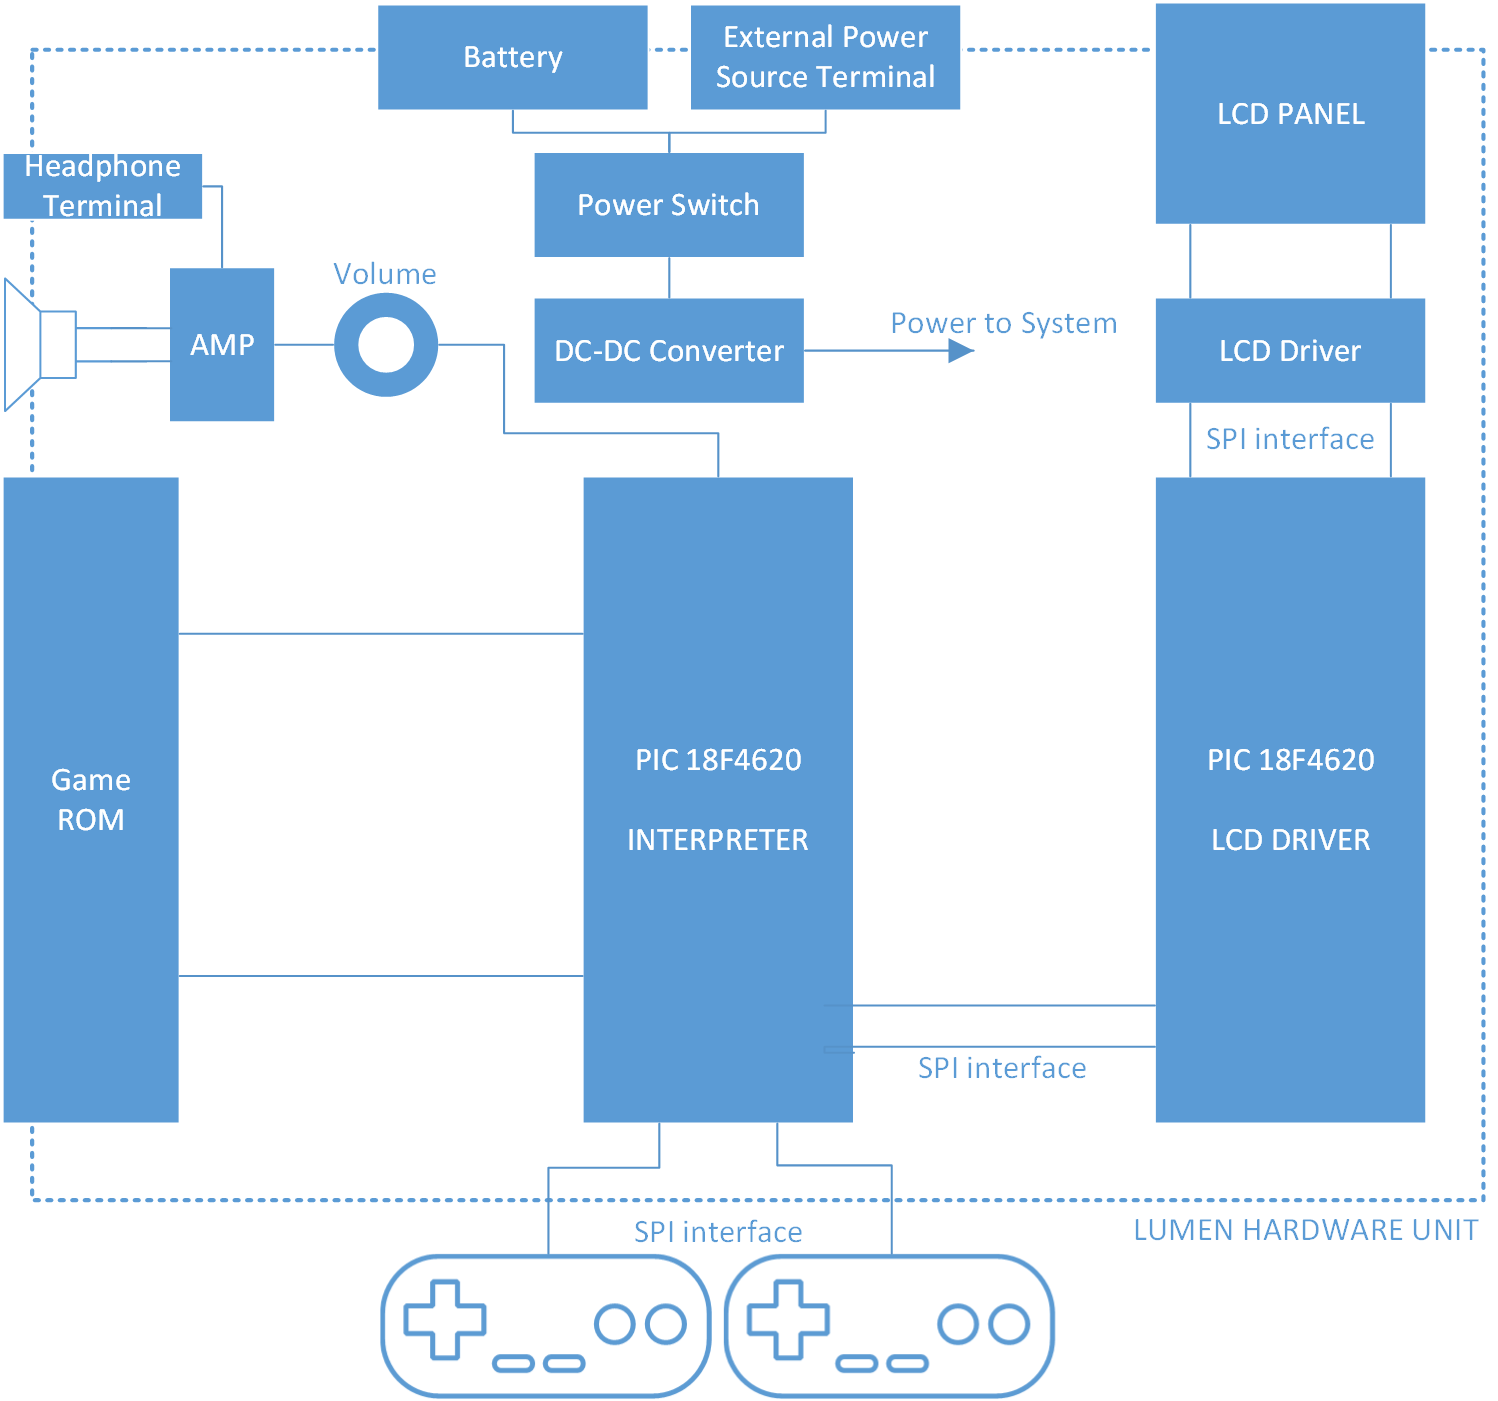
\includegraphics[width=0.9\textwidth]{GameConsole/LumenGameConsoleOverview.PNG}
		\caption{Console Overview}\par
		\label{fig:LumenGameConsoleOverview}
	\end{figure}

\newpage
\section{Controller}
	\subsection{Overview}
		\par A total of 8 push buttons are present on the controller, each with a pressed and a released state. When the user presses a button the state changes form released to pressed and vice versa. The controller uses an SPI interface to allow communication with the game.
		Multiplayer is possible when connecting 2 controllers at once.

		\begin{figure}[H]
			\centering
			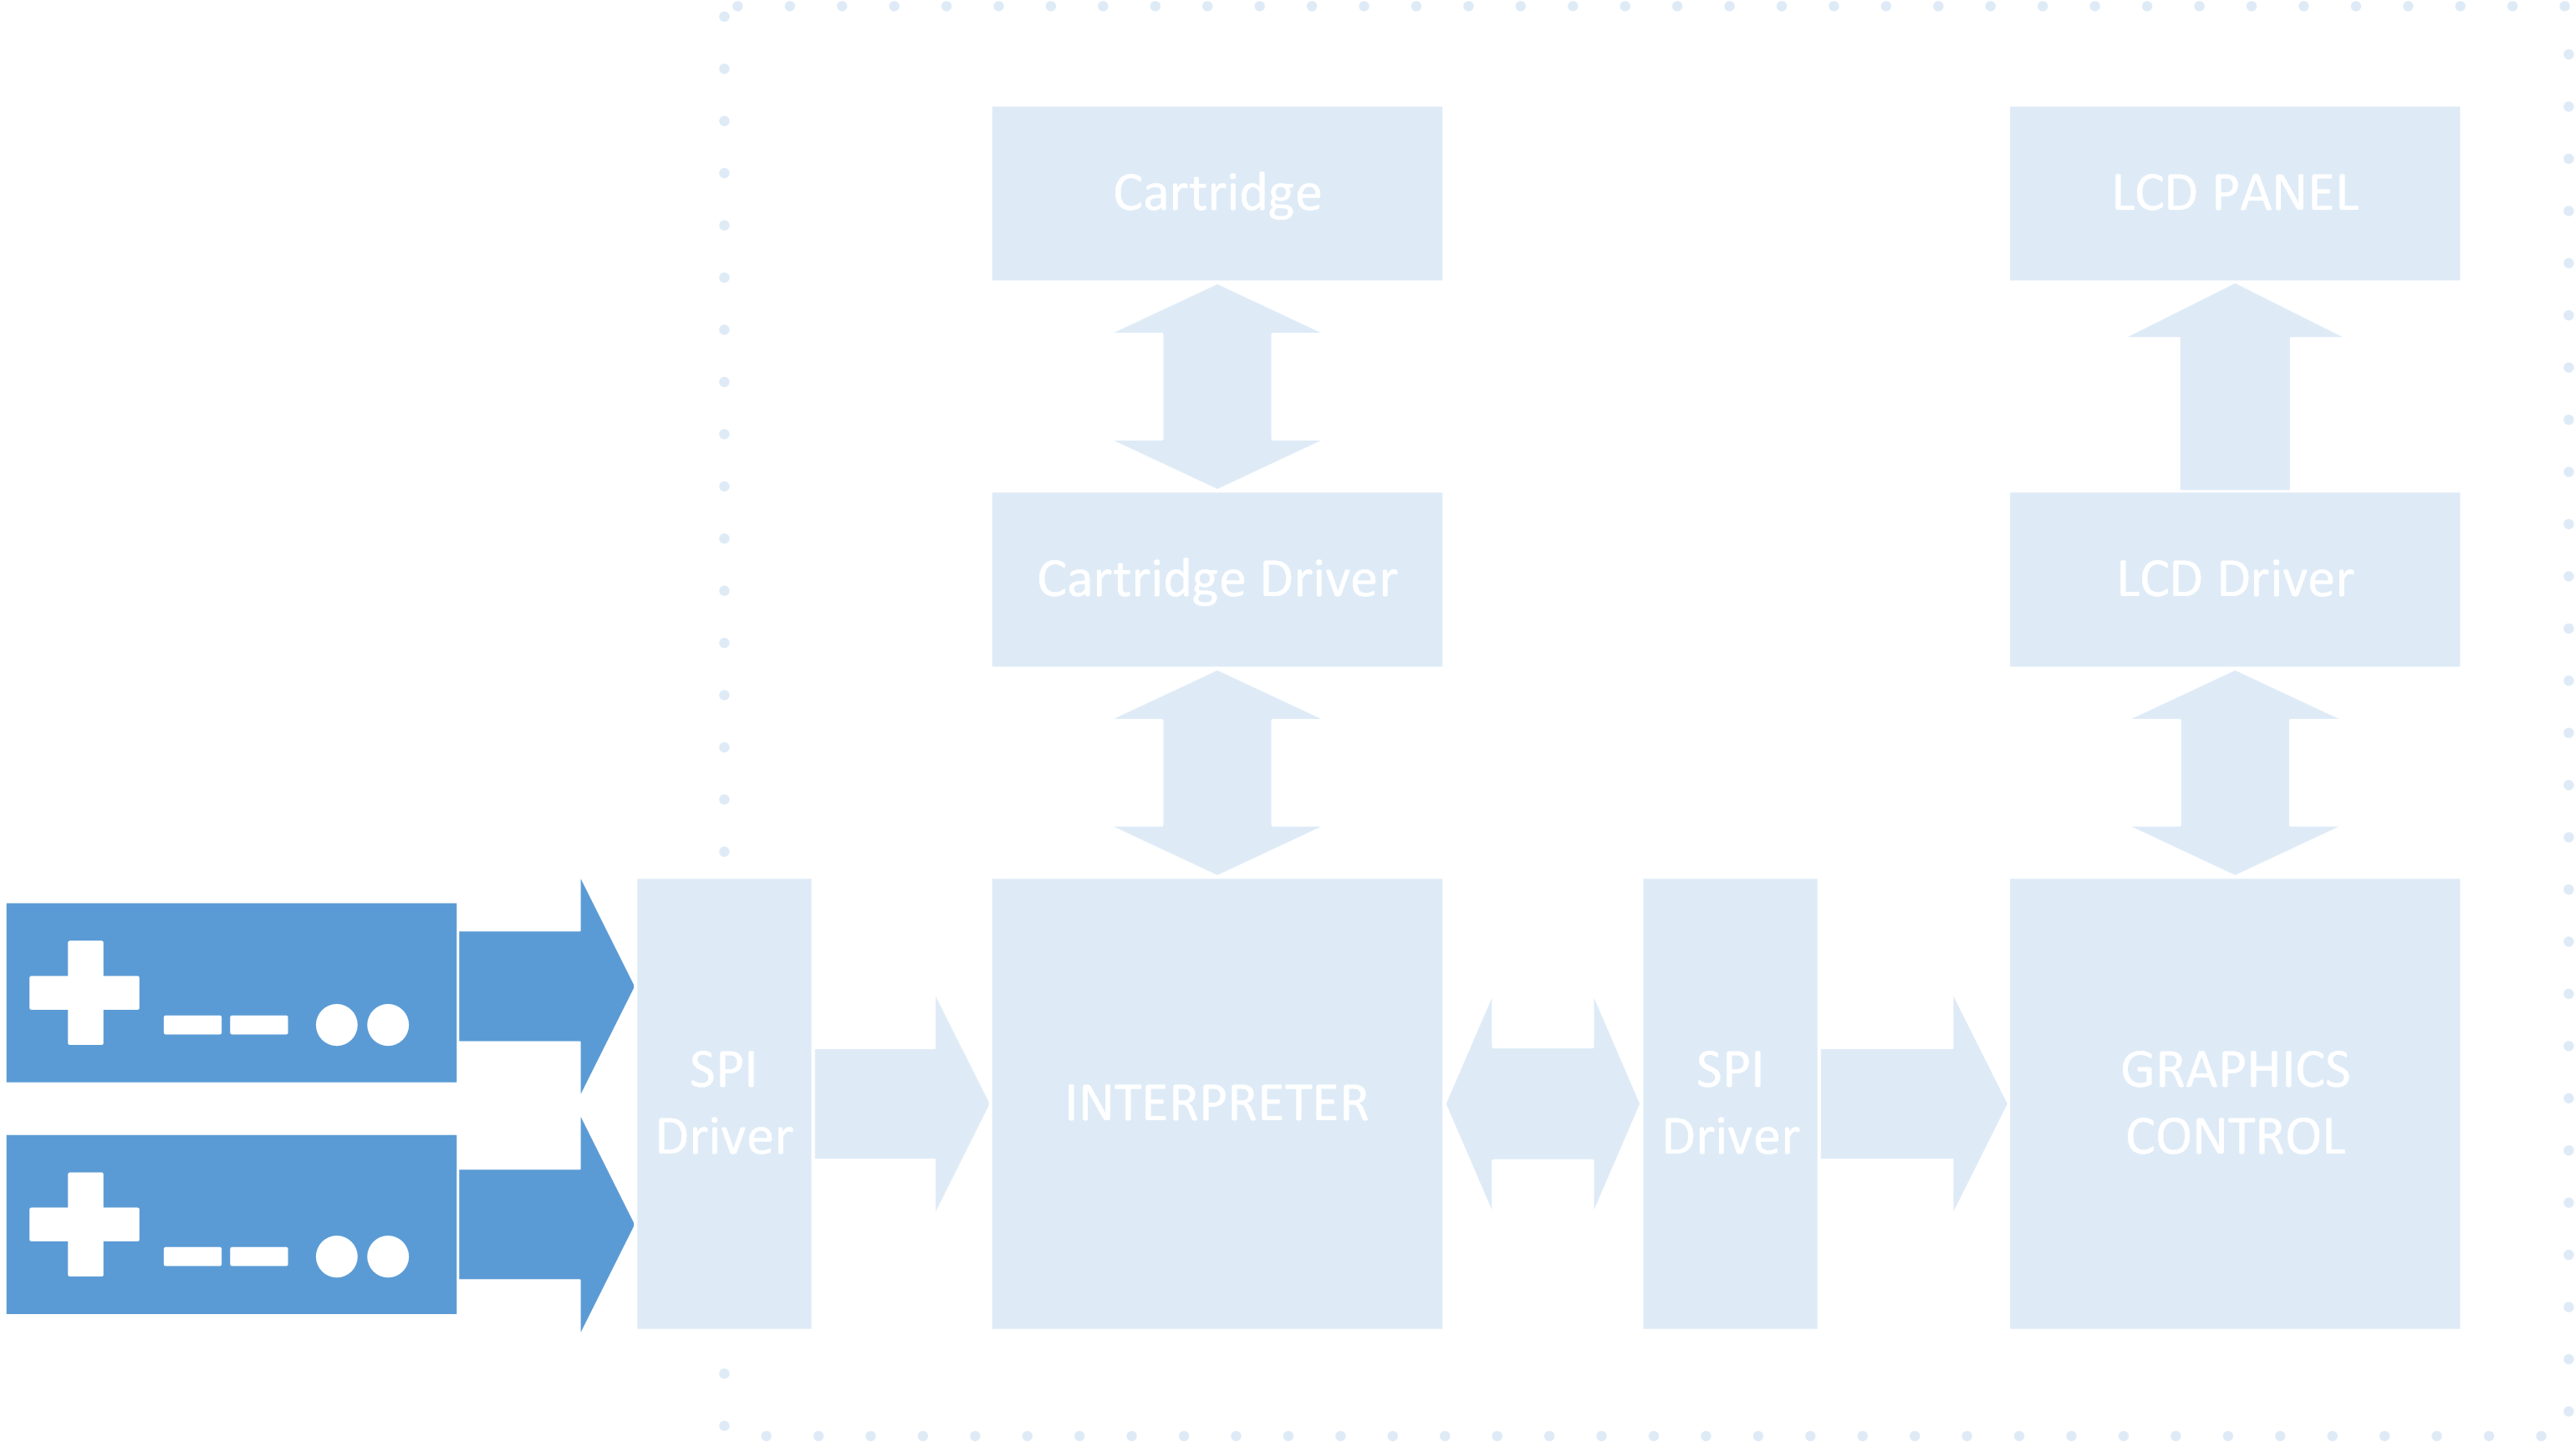
\includegraphics[width=0.4\textwidth]{GameConsole/Controllers_overview.PNG}
			\label{fig:ControllerOverview}
		\end{figure}

	\subsection{Buttons}
		\subsubsection{D-Pad}
			\par Four of the buttons at the left side of the controller are formed as a D-Pad, a flat thumb-operated four-way directional control with one push button on each point,
			providing intuitive direction and steering capabilities, and should be used as such.

		\subsubsection{Select and start}
			\par In the center, the select and start button are located.
			These should be used to start the game, pause it, allow menu navigation etc.
			The start button should allow pausing the game at any point, pressing start again returns to the game.

		\subsubsection{A and B}
			\par Next to the select and start buttons, A and B are located.
			These two buttons are to be used in-game, providing interaction with objects on the screen.
			They should not be used to pause or unpause the game at any time.

	\subsection{Interface}
		\par The controller connects through a three-wire interface similar to SPI. A maximum of two controllers can be connected, addressed as 0 and 1. The timing can be seen in this view (clockperiod of 6$\mu$s, from top to bottom: Latch, Clock, Data):

		\begin{figure}[H]
			\centering
			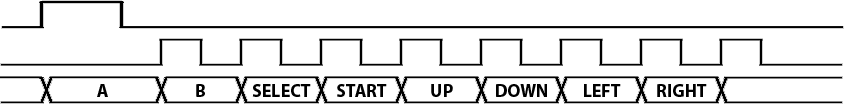
\includegraphics[width=0.7\textwidth]{GameController/ControllerInterface.PNG}
			\caption{Interface timing of the controller}\par
			\label{fig:ControllerInterface}
		\end{figure}

\section{Interpreter}
	\subsection{Overview}
		\par The interpreter is the main unit of the console. It executes the code and sends commands to the graphics controller to ensure the data displayed on screen is correct.
		Since the code is stored in external cartridge memory in the form of bytecode, specific requirement should be met to obtain accurate behaviour:
		\begin{itemize}
			\item MCU: PIC18F4620 (8-bit, 8 MHz)
			\item RAM: 3968 bytes - 256 bytes can be used by one game
			\item Input: NES controller (max 2)
		\end{itemize}

		\begin{figure}[H]
			\centering
			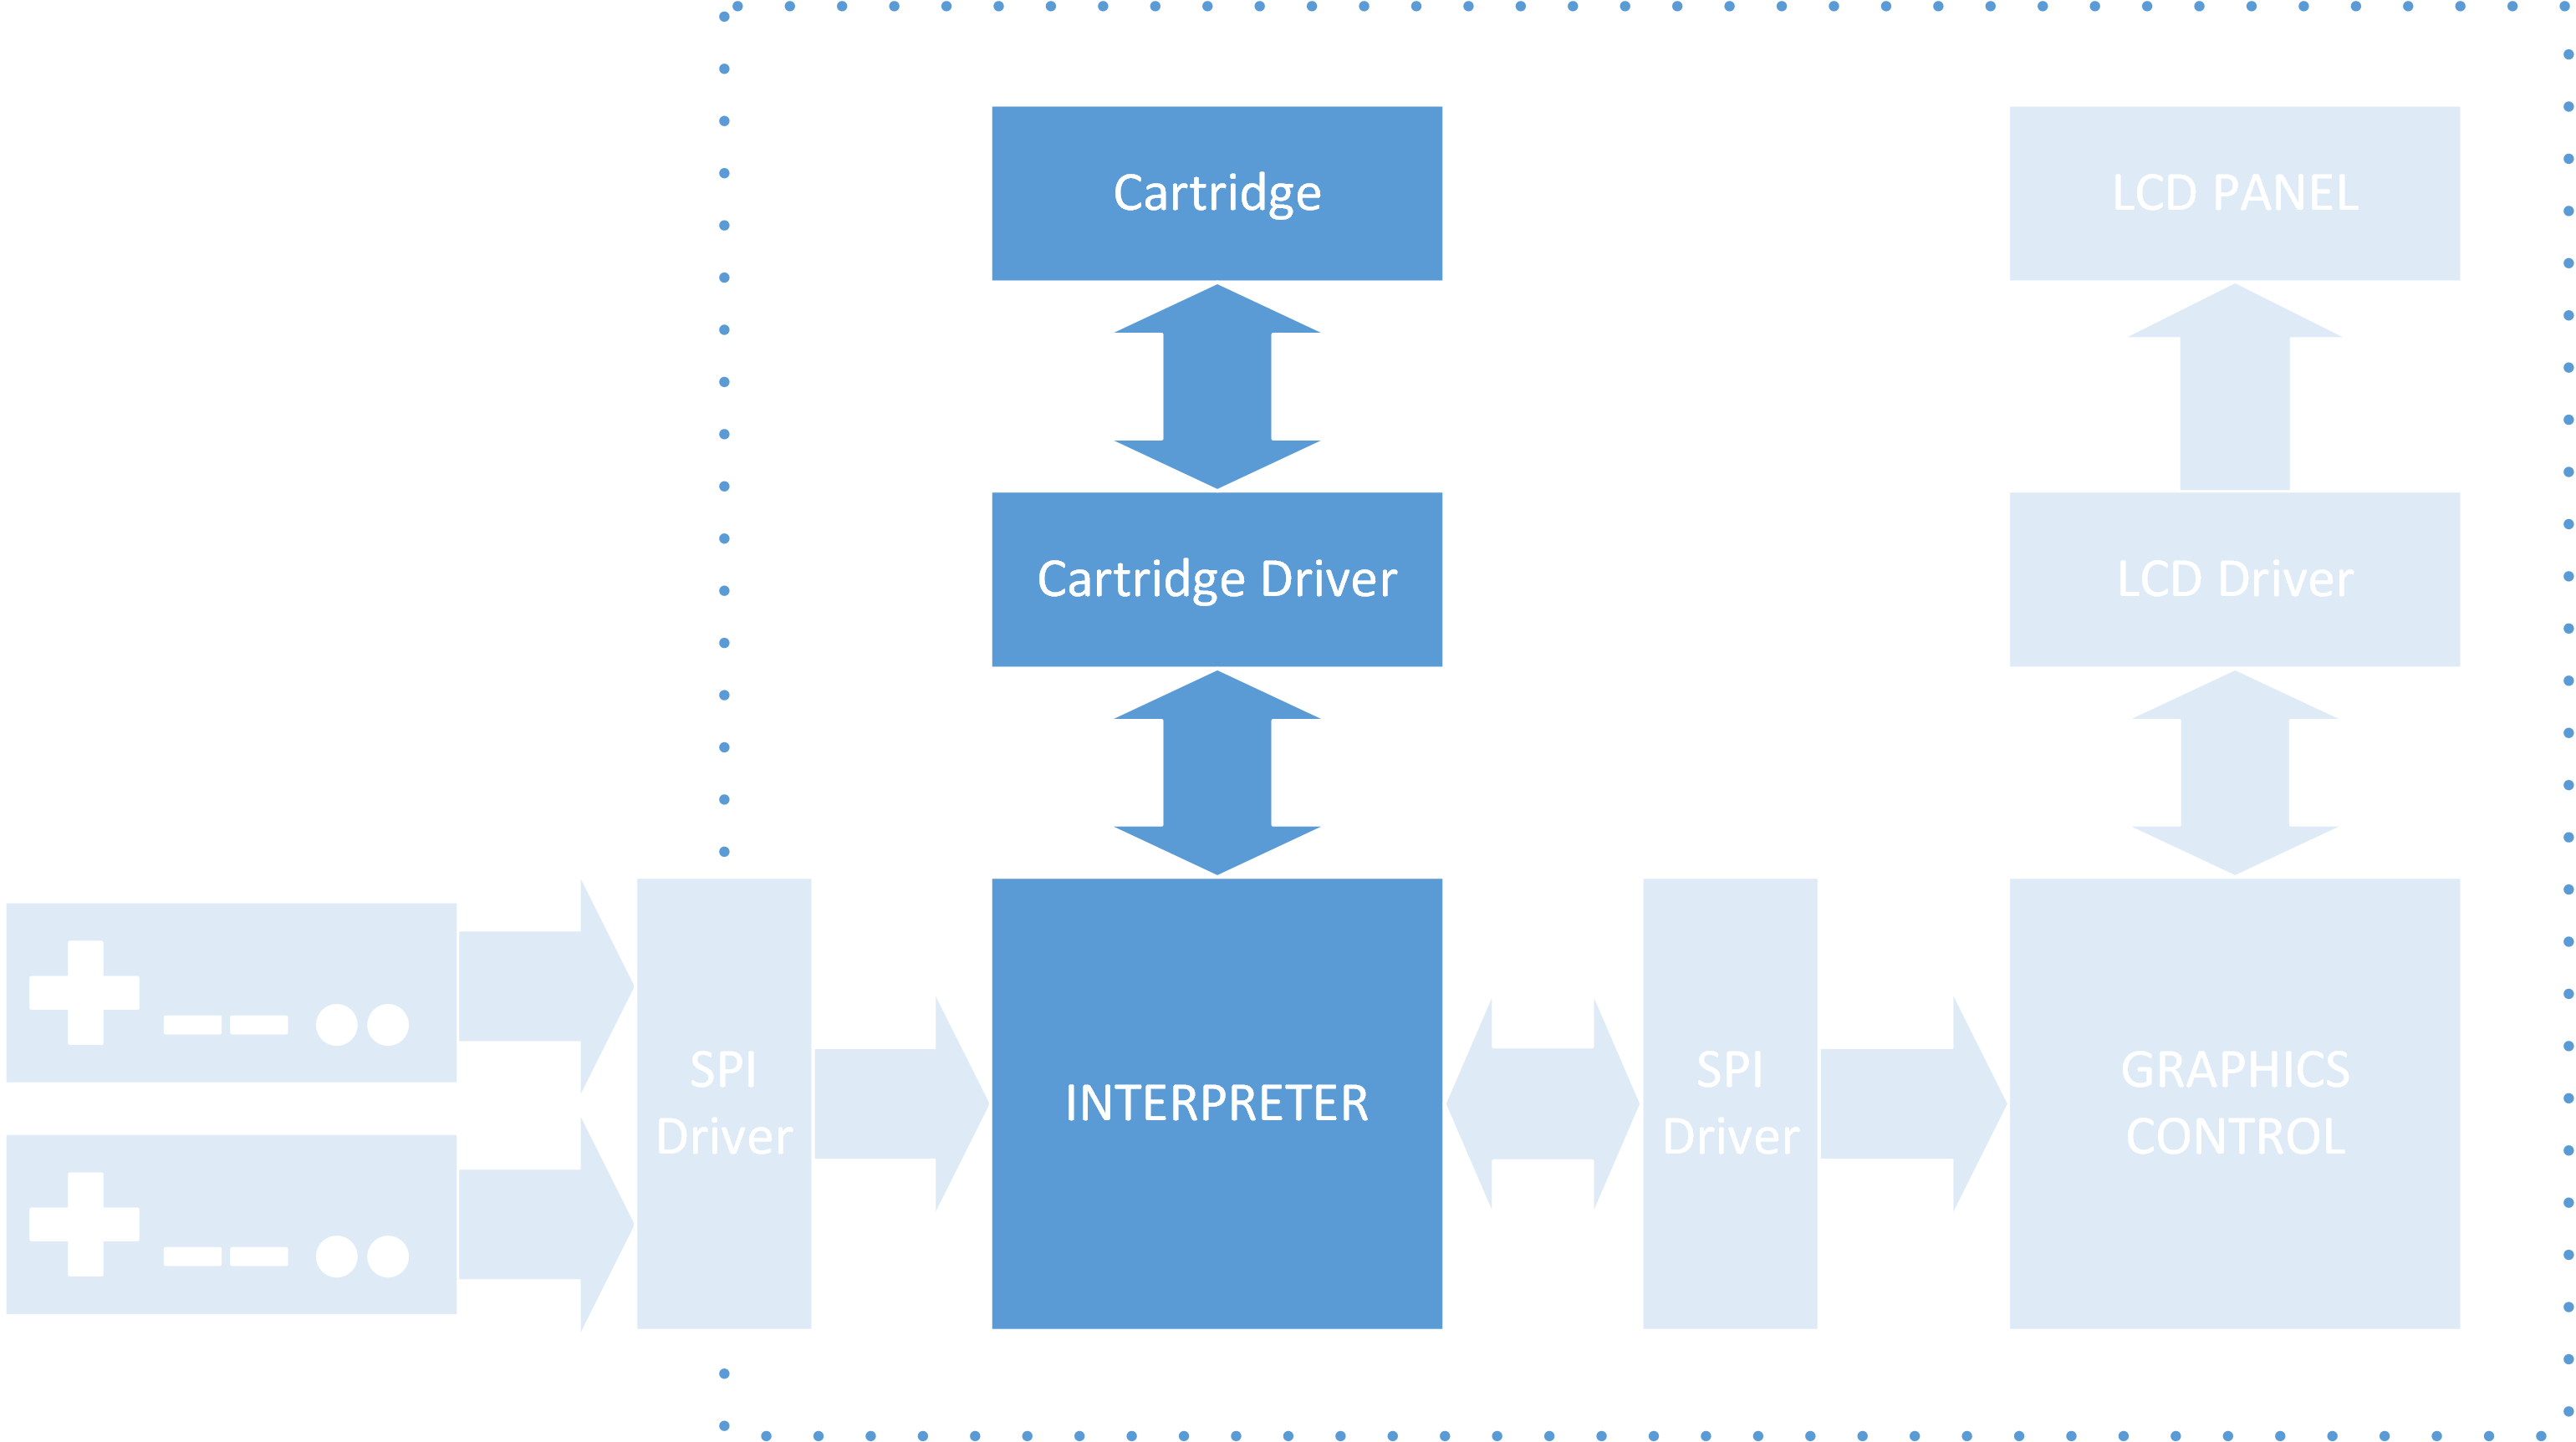
\includegraphics[width=0.4\textwidth]{GameConsole/Interpreter_overview.PNG}
			\label{fig:InterpreterOverview}
		\end{figure}

	\subsection{Peripherals}
		\subsubsection{Registers}
			\par Data transfer and manipulation is done via registers.
			These are memory locations that can be used to perform arithmetics on, used as delay counter\ldots
			They can be used as data storage, but the RAM is a better place for this.
			In total, 16 8-bit wide registers can be used, yet one should be used with caution since it will be overwritten by some specific instructions.
			Registers 0 to 14 are free to use, and will only be overwritten when the code tells the interpreter to do so.
			The 15th register, called the HL register, is used by the interpreter as data buffer for e.g. reading a controller or timer.

		\subsubsection{Stack}
			\par The stack is used to temporarly store data when the interpreter executes a subroutine or a register should be stored for later use.
			It is a LIFO structure of 256 items long, each item being 8 bit wide.
			The stack pointer is 8 bit too, but cannot be manipulated by the user directly: push and pop instructions are supported, and are available through the interpreter.

		\subsubsection{Program counter}
			\par The program counter is a pointer to where the interpreter is in the code.
			It is a 16 bit unsigned short, starting at 0 for the first instruction.
			Each instruction or operand increments this program counter.
			The program counter cannot be manipulated by the user directly, but should go through the jump, call or return instructions of the interpreter.
			A jump instruction replaces the program counter by a new value, while the call instruction pushes the current program counter to the stack and then replaces the program counter by the new one.
			Return pops the program counter from the stack at the end of a subroutine, and replaces the current program counter by this value, which results in a return to the point of calling the subroutine.

		\subsubsection{RAM}
			\par RAM can be used to store data during the execution of a program, it is 256 items long, each item being 8 bits wide.
			It will never be overwritten by the interpreter automatically, yet overwriting can happen when the code tells the interpreter to do so.
			It is possible to exchange data from a register to a RAM address and the other way around.
			Data that should be stored over a longer period of time can be placed in RAM, and copied back to a register for later manipulation.

	\subsection{Cartridge memory mapping}
		\par An important aspect of every game is the memory mapping on the cartridge.
		Every item (code, sprites, strings and maps) has its own specific start- and endaddress to establish a solid and correct performance. The mapping is as follows:

		\begin{figure}[H]
			\centering
			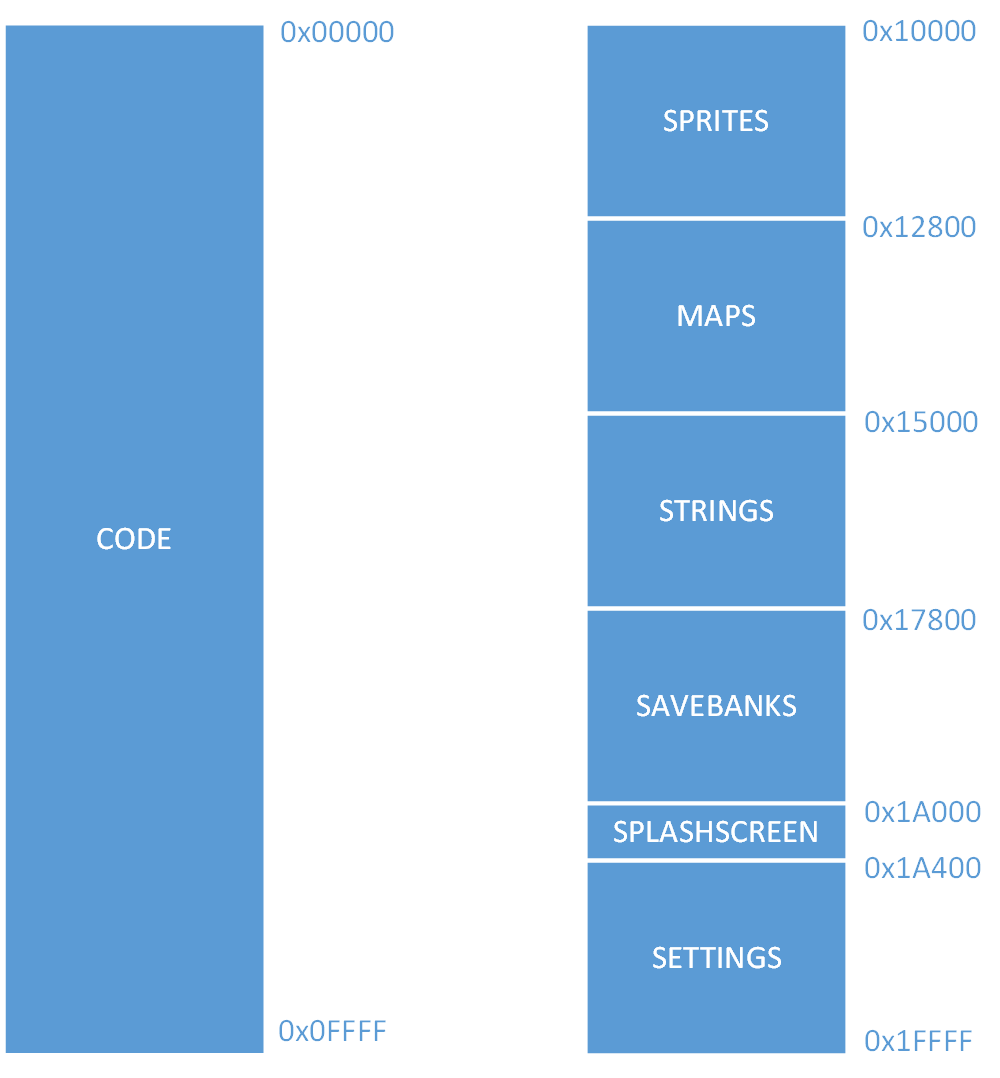
\includegraphics[width=0.65\textwidth]{GameConsole/MemoryMap.PNG}
			\caption{Memory map of the cartridge}\par
			\label{fig:MemoryMap}
		\end{figure}

		\subsubsection{Code}
			\par This is the actual bytecode that will be interpreted and executed. An in-depth look on the instructionset can be found in chapter~\ref{cha:InstructionSet}. The maximum codesize is 64kB, or 65536 bytes. If no jump is performed at byte 65535, the program counter will overflow, resulting in a reset of the program counter to zero. Code examples can be found in the appendix.

		\subsubsection{Sprites}
		\label{subsec:sprites}
			\par A sprite is an 8 by 8 pixels bitmap in black and white. Each bit represents one pixel, resulting in a size of 8 bytes per sprite.
			The addressing starts at the top left, and goes down per colum, this happens to be 8 bits, and can thus be packed in one byte.
			The first colum is the first byte, the second colum the second byte\ldots

			\begin{table}[h]
			\centering
				\begin{tabular}{m{0.2em} m{0.2em} m{0.2em} m{0.2em} m{0.2em} m{0.2em} m{0.2em} m{0.2em} cccccccccc}
					$\square$      & $\square$      & $\blacksquare$ & $\blacksquare$ & $\blacksquare$ & $\blacksquare$ & $\square$      & $\square$      &&& 0 & 0 & 1 & 1 & 1 & 1 & 0 & 0 \\
					$\square$      & $\blacksquare$ & $\square$      & $\square$      & $\blacksquare$ & $\blacksquare$ & $\blacksquare$ & $\square$      &&& 0 & 1 & 0 & 0 & 1 & 1 & 1 & 0 \\
					$\blacksquare$ & $\square$      & $\square$      & $\blacksquare$ & $\blacksquare$ & $\blacksquare$ & $\blacksquare$ & $\blacksquare$ &&& 1 & 0 & 0 & 1 & 1 & 1 & 1 & 1 \\
					$\blacksquare$ & $\square$      & $\blacksquare$ & $\blacksquare$ & $\blacksquare$ & $\blacksquare$ & $\blacksquare$ & $\blacksquare$ &&& 1 & 0 & 1 & 1 & 1 & 1 & 1 & 1 \\
					$\blacksquare$ & $\blacksquare$ & $\blacksquare$ & $\blacksquare$ & $\blacksquare$ & $\blacksquare$ & $\blacksquare$ & $\blacksquare$ &&& 1 & 1 & 1 & 1 & 1 & 1 & 1 & 1 \\
					$\blacksquare$ & $\blacksquare$ & $\blacksquare$ & $\blacksquare$ & $\blacksquare$ & $\blacksquare$ & $\blacksquare$ & $\blacksquare$ &&& 1 & 1 & 1 & 1 & 1 & 1 & 1 & 1 \\
					$\square$      & $\blacksquare$ & $\blacksquare$ & $\blacksquare$ & $\blacksquare$ & $\blacksquare$ & $\blacksquare$ & $\square$      &&& 0 & 1 & 1 & 1 & 1 & 1 & 1 & 0 \\
					$\square$      & $\square$      & $\blacksquare$ & $\blacksquare$ & $\blacksquare$ & $\blacksquare$ & $\square$      & $\square$      &&& 0 & 0 & 1 & 1 & 1 & 1 & 0 & 0 \\
				\end{tabular}
			\end{table}
			
			This sprite, representing a ball, has the binary representation in the right table.
			Since we address by colum, the first byte is 0b00111100, which corresponds to 0x3C.
			The second colum is 0b01001110, and thus 0x4E.
			When all pixels are calculated the bytes are placed after one another, resulting in a complete sprite, here 0x3C4E9FBFFFFF7E3C.

		\subsubsection{Maps}
			\par A map is a combination of sprites that can fill the background of the screen.
			Placing a map on the screen can be functional, e.g. in a platformer game, or aesthetically.
			It is in fact a tiled field containing the indexes of sprites in the onscreen memory, each tile being 8 by 8 pixels (equal to 1 sprite).
			For more information on maps, please refer to the chapter~\ref{subsec:maps}.

		\subsubsection{Strings}
			\par Strings can be used to be drawn on screen as guidelines or instructions to the user.
			They are to be stored in the cartrigde memory as null-terminated ascii encoded strings, and will be read as such.
			If a string is not null-terminated, the interpreter will read until the first null is encountered, which can result in unexpected behaviour.
			A maximun total size of 10kB of strings can be loaded into the ROM, yet that amount can never be displayed at once on the screen, since the string buffer is limited to 256 bytes.
			For more information on strings, refer to the chapters~\ref{subsec:stringdata} and ~\ref{subsec:strings}.

		\subsubsection{Savebanks}
			\par The savebanks are 10 address locations of each 1kB that can be used freely by the game.
			If playernames, highscores, achievements\ldots should be stored, this is the location to do so.
			The game will not check if the data is legitimate or not, this is up to the programmer.
			Settings should not be stored in savebanks, for this has its own address location.

		\subsubsection{Splash screen}
			\par A splash screen is the screen that should be shown while all data is loaded and transfered between the interpreter and the graphics control.
			It has to be a black and white bitmap addressed from the top left down each colum.
			Since the screen is 84x48, a fullscreen bitmap is 4032 bits, or 504 bytes.

		\subsubsection{Settings}
			\par Settings can be stored in this address location.
			No restrictions are applied, and the content is up to the programmer.

\section{Graphics control}

	\begin{figure}[H]
		\centering
		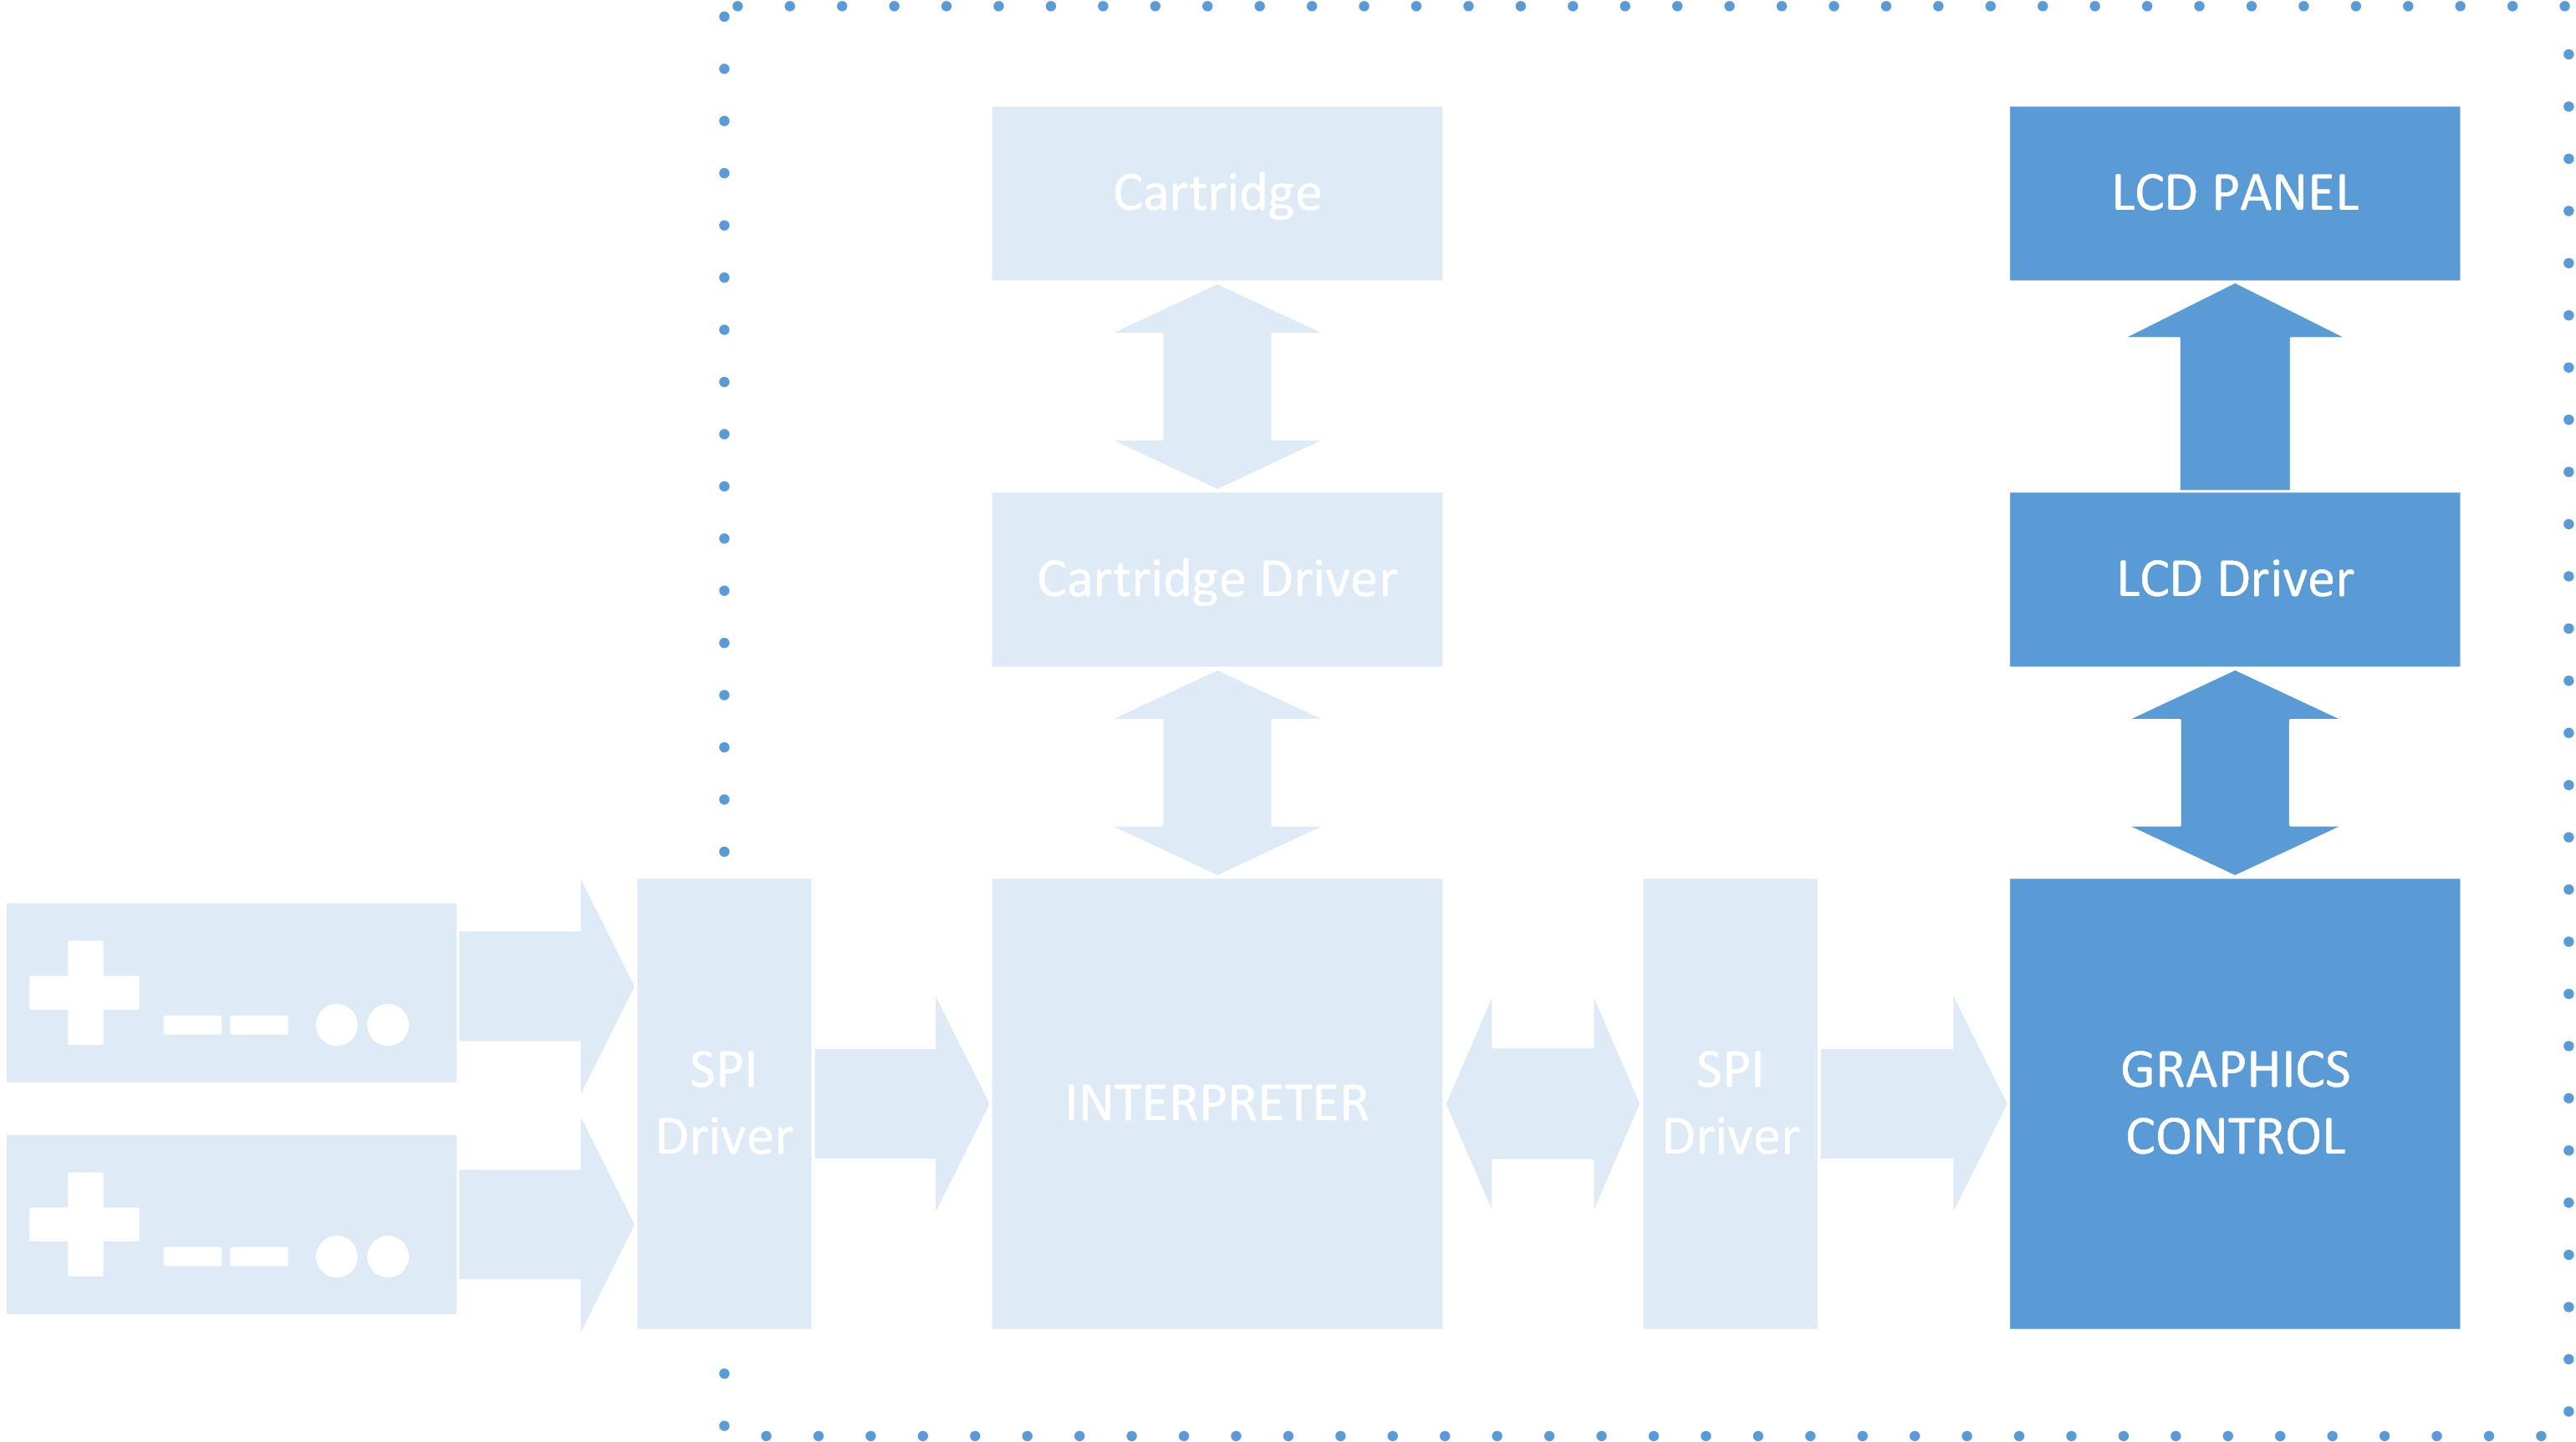
\includegraphics[width=0.4\textwidth]{GameConsole/GraphicsControl_overview.PNG}
		\label{fig:GraphicsControlOverview}
	\end{figure}

\chapter{The graphics control}
\label{cha:GraphicsControl}

\section{Overview}
	\par The graphics control is located entirely in a separate microcontroller. Its tasks in a nutshell are to drive the actual LCD display and to provide a simple way of using graphics in a game. To do so it provides a set of commands to the programmer that can be used to initialize, draw, move and remove spites on the screen. It also has support for text on screen and for maps that can be scrolled over the screen.

\section{The LCD display}
	\par The LCD display used in this setup has a resolution of 84x48 pixels. It has a PCD8544 chipset and is interfaced with SPI. The chipset does all the timing and scanning of the LCD. All we need to provide is a correct initialisation, fill the VRAM and send valid commands. This is where graphics control comes in. The graphics control translates SPI commands and data from the interpreter to SPI commands and data the LCD understands.

\section{Memories of the graphics control}
	\par The graphics control has several sort of memories. Although most of it is directly in ram, their purposes are completely different:

	\subsection{Sprites in memory}
		\par This part of the memory is used to store the actual data of a sprite, or the data for the visual representation of that particular sprite. It can contain up to 32 different sprites and a sprite is 8 by 8 pixels or 8 bytes in size. For an in-depth look on the format of sprites, please refer to chapter~\ref{subsec:sprites}.

		\par Every sprite in memory can be referenced by its number in memory, as there are 32 possible sprites valid numbers are from 1 up to 32.

	\subsection{Sprites on screen}
		\par This part of the memory tell the graphics control what to draw where concerning sprites. It can contain up to 32 record. A record is 3 bytes big and represents a sprite (first byte), a X position on the screen (second byte) and a Y position on the screen (third byte). From now on a sprite can be drawn on the screen. And a sprite on the screen is referenced by a list number, that number is the number of the record containing information of the sprite data and position. Note that multiple records can use the same sprite.

	\subsection{Maps}
	\label{subsec:maps}
		\par This part of the memory is used for background maps. Up to four maps can be used. A map exists of tiles and these tiles are in fact just sprites. One must use the the number of the spite in memory to use it in a map. A map measures 16 by 8 tiles, or 128 by 64 pixels. For tiling the map a sequence of references to sprites is needed. A map is tiled from left to right and than from top to bottom. When drawing a map on the screen, one can give a X and Y offset, resulting in a scrollable background.

	\subsection{Strings}
	\label{subsec:strings}
		\par This part of the memory is used to store pointers to string data. A string starts at the pointer location and ends when a null character is encountered. A maximum of 32 strings is allowed. The number of the string is used for referencing when drawing it to the screen.

	\subsection{String data}
	\label{subsec:stringdata}
		\par This part of the memory is used to store the actual data for the strings. It can contain up to 256 characters. Therefore all the strings (including null characters) together can have a maximum size of 256 bytes. A new string starts where the old string ended. Therefore it is important to initialize the strings at the beginning. Otherwise conflicts of overwriting strings is a ever present danger.

	\subsection{Font}
		\par This part of the memory contains the data for the actual graphical representation of a ascii character on the screen. A character is made of five bytes, and is mapped onto a 5x7 font. This part is also the only part not in RAM, it is hard coded in the flash region of the microcontroller.

	\subsection{VRAM}
		\par This part of the memory is of uttermost importance, this is where everything containing some graphic content different from text is drawn. It is used as sort of double buffer. In this part of the memory the final image is rendered. First the background map is drawn onto it, if needed. Then the sprites are drawn onto it. Once a full image is complete it is send to the LCD where it remains in its VRAM until a new image is send.

	\subsection{TRAM}
		\par This part of the memory is used to display text on the screen. To show text on the screen the graphics control receives numbers corresponding to the ascii standard. These numbers are converted to graphical data trough the font memory. When sending the image to the screen, the text data is combined with the graphics data by means of a XOR operation. So the text is black on a white background and white on a black background.
\section{The normal operation}
	\par The normal way to go is to initialize the graphics control using its provided initializer. This takes care of correct reset timings for the LCD. From then on the graphics control is ready to receive data. This data is received over SPI and the data received will be seen as a command followed by some arguments if necessary. Correct operation is not guaranteed when synchronisation is lost or when faulty commands are send. Correct commands are:
	\begin{tabular}{r|l}
		Command & Description \\
		Load sprite: 0x10 & Load a sprite in sprite memory \\
		Load map: 0x12 & Load a map in map memory \\
		Load string: 0x14 & Load a string in string memory \\
		Set sprite: 0x16 & Initialize a sprite in sprites on screen memory \\
		Update sprite: 0x18 & Draw a sprite on the screen at a certain position \\
		Clear sprite: 0x1A & Remove a sprite from the screen \\
		Draw map: 0x1C & Draw a map on the screen with a certain offset \\
		Draw string: 0x1E & Draw a string on the screen at a certain position \\
		Clear all: 0x20 & Clear both VRAM and TRAM \\
		Clear graphics: 0x22 & Clear VRAM \\
		Clear strings: 0x24 & Clear TRAM \\
		Redraw: 0x26 & Send the VRAM and TRAM to the LCD \\
		All on: 0x28 & Turn all the pixels on, draw them all black \\
		All off: 0x2A &  Turn all the pixels of, draw them white\\
		Invert: 0x2C &  Enable the inverted mode, black is white and vice versa\\
		Normal: 0x2E &  Enable normal mode, to restore from inverted mode\\
	\end{tabular}
	The reception of SPI communication is done in the background by interrupts. In the foreground a routine constantly checks for new commands. If a command is received the routine waits for the needed arguments, and then it calls the corresponding function.




  \chapter{The Game Controller}
\label{cha:gameController}

The interpreter uses two handheld gamepads allowing user input for the running code to be acquired. Since two controllers can be connected at the same time, a multiplayer game can be developped using feedback from two different players. The interpreter does not check for keypresses itself, this is something the programmer has to poll for.
The controllers used are originally from a NES console. These controllers use SPI to communicate, and allow for more time to be spared on the console, since no development needs to be done anymore.

\section{Overview}
A total of 8 push buttons are present on the controller, all accessible by the user. Each button has two states, a pressed-state and a released-state. When the user presses a button the state changes form released to pressed and vice versa. The controller uses an SPI interface to allow communication with the game. The exact button states can be retreived once the interpreter is running.

\begin{figure}[h]
    \centering
	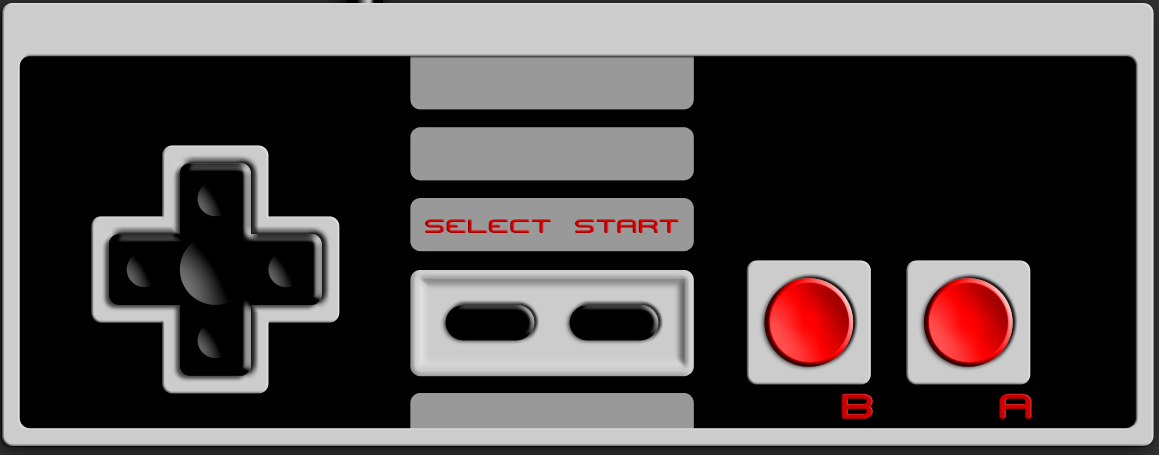
\includegraphics[width=0.7\textwidth]{GameController/GameControllerPicture.PNG}
    \caption{Game controller}\par
    \label{fig:GameController}
\end{figure}

\section{Buttons}
\subsection{D-Pad}
Four of these are formed as a D-Pad, a flat thumb-operated four-way directional control with one push button on each point, providing intuitive direction and steering capabilities, and should be used as such to provide a common interface for all developed games.

\subsection{Select, start}
In the center, the select and start button are located.
These should be used to start the game, pause it, allow menu navigation etc.
The start button should allow pausing the game at any point, pressing start again returns to the game.

\subsection{A and B}
Next to the select and start buttons are A and B located.
These two buttons are to be used in-game, providing interactivity with objects on the screen, and should not be used to pause or unpause the game at any time.
This can mean jumping on or over an obsacle, toggling a setting, opening a box\ldots

\section{Interface}
The controller is interfaced though a three-wire interface (with additional power and ground connections), equivalent to SPI.
A maximum of two controllers van be connected, and they are to be addressed as controller 0 and 1. The timing can be seen in this view:

\begin{figure}[h]
    \centering
	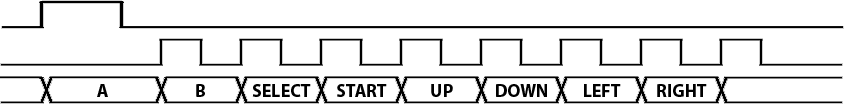
\includegraphics[width=\textwidth]{GameController/ControllerInterface.PNG}
    \caption{Interface timing of the controller}\par
    \label{fig:GameController}
\end{figure}
  \chapter{The register organisation}
\label{cha:RegisterOrganisation} 

\par \noindent The LUMEN interpreter provides two register banks directly accessible by the programmer. One register bank is reserved for the 8-bit 
instructions and the other register, the 32-bit register is used for the floating point operations. Each register bank contains 16 registers.
15 registers are general purpose and one register is the accumulator register. \bigskip

\par \noindent The program counter register points to the next instruction to be executed in the program memory. The stack pointer register points to the current
stack position. 

\subsection {8-bit register bank}
\par \noindent The 8-bit register bank consist out of 16 8-bit registers, R0, R1, \ldots , R14 and a special HL register. The HL register, also known as 
the accumulator register contains results given by several instructions and should not be used to store values. Only 8-bit unsigned integers can be 
stored in these registers. 

\subsection{32-bit register bank}
\par \noindent The 32-bit register bank consist out of 16 32-bit registers, R0, R1, \ldots , R14 and a special HL register. The HL register, also known as 
the accumulator register contains results given by several instructions and should not be used to store values. Only 32-bit  single precision floats 
can be stored in these registers. Pushing values of the register to the stack is only possible with a special instruction.

\subsection {Program counter register}
\par \noindent The program counter is a 16-bit register. On power up the program counter is initialized to address 0x0000 and the instruction find
 on this location in ROM is executed. From this point on the program counter is controlled indirectly by the program instructions themselves 
 that were generated by the programmer. 

\subsection{Stack pointer register}
\par \noindent The stack pointer register is a 8-bit register and used to keep track of the top of the stack. The stack is used for saving variables, returning 
addresses, passing arguments to subroutines and various other uses that might be conceived by the programmer. The instructions PUSH and CALL put 
information onto the stack. The instruction POP takes information off the stack. \bigskip

\par \noindent As information is put onto the stack, the stack grows downwards in RAM memory. As a result, the stack pointer should always be pointing at the highest
location of RAM space that has been allocated to use by the stack. On power-up the stack pointer is initialized to 0x00.
  \chapter{Instruction Set}
\label{cha:InstructionSet}

Each LUMEN instruction is a 8-bit byte divided into an OPCODE which specifies the instruction
type and one or more operands which further specify the operation of the instruction. These operands
are also 8-bit. The LUMEN instruction summary in described in this chapter lists the instructions recognized by the 
LUMEN compiler. The instructions set can be grouped in 7 basic categories:

	\begin{itemize}
		  \item Variable manipulation
		  \item Mathematical operations
		  \item Logic manipulation
		  \item Calls and Jumps
		  \item Stack manipulation
		  \item Graphics
		  \item Sounds
	\end{itemize}

\noindent All instructions are executed in one single instruction cycle, unless a conditional test is true
or the program counter is changed as a result of an instruction. In these cases the execution takes two instruction
cycles with the second cycle as an NOP. One instruction cycle consist out of XXX clock cycles.

\newpage
\begin{table}[h]
\begin{tabular}{llllll}
Mnemonic & Operands & Operation & Affected & Opcode & Cfr.\\
LD & Op1: RegisterOp2: 8 bit unsigned integer, &  &  & 0x00 & \pageref(subsec:LD_instruction)\\
CPY & Op1: RegisterOp2: Register, &  &  & 0x01 & \pageref(subsec:CPY_instruction)\\
ST & Op1: RAM addressOp2: Register, &  &  & 0x02 & \pageref(subsec:ST_instruction)\\
STI & Op1: RAM addressOp2: 8 bit unsigned integer, &  &  & 0x03 & \pageref(subsec:STI_instruction)\\
LR & Op1: RegisterOp2: RAM address, &  &  & 0x04 & \pageref(subsec:LR_instruction)\\
EQU & Op1: RegisterOp2: Register, &  &  & 0x05 & \pageref(subsec:EQU_instruction)\\
GT & Op1: RegisterOp2: Register, &  &  & 0x06 & \pageref(subsec:GT_instruction)\\
LT & Op1: RegisterOp2: Register, &  &  & 0x07 & \pageref(subsec:LT_instruction)\\
ADD & Op1: RegisterOp2: Register, &  &  & 0x08 & \pageref(subsec:ADD_instruction)\\
ADDI & Op1: RegisterOp2: 8 bit unsigned integer, &  &  & 0x09 & \pageref(subsec:ADDI_instruction)\\
SUB & Op1: RegisterOp2: Register, &  &  & 0x0A & \pageref(subsec:SUB_instruction)\\
SUBI & Op1: RegisterOp2: 8 bit unsigned integer, &  &  & 0x0B & \pageref(subsec:SUBI_instruction)\\
MUL & Op1: RegisterOp2: Register, &  &  & 0x0C & \pageref(subsec:MUL_instruction)\\
MULI & Op1: RegisterOp2: 8 bit unsigned integer, &  &  & 0x0D & \pageref(subsec:MULI_instruction)\\
DIV & Op1: RegisterOp2: Register, &  &  & 0x0E & \pageref(subsec:DIV_instruction)\\
DIVI & Op1: RegisterOp2: 8 bit unsigned integer, &  &  & 0x0F & \pageref(subsec:DIVI_instruction)\\
INC & Op1: Register, &  &  & 0x10 & \pageref(subsec:INC_instruction)\\
DEC & Op1: Register, &  &  & 0x11 & \pageref(subsec:DEC_instruction)\\
PWR & Op1: RegisterOp2: Register, &  &  & 0x12 & \pageref(subsec:PWR_instruction)\\
PWRI & Op1: RegisterOp2: 8 bit unsigned integer, &  &  & 0x13 & \pageref(subsec:PWRI_instruction)\\
SQRT & Op1: Register, &  &  & 0x14 & \pageref(subsec:SQRT_instruction)\\
LOG & Op1: RegisterOp2: Register, &  &  & 0x15 & \pageref(subsec:LOG_instruction)\\
LOGI & Op1: RegisterOp2: Fixed value, &  &  & 0x16 & \pageref(subsec:LOGI_instruction)\\
RAND & Op1: RegisterOp2: Register, &  &  & 0x17 & \pageref(subsec:RAND_instruction)\\
RANDI & Op1: 8 bit unsigned integerOp2: 8 bit unsigned integer, &  &  & 0x18 & \pageref(subsec:RANDI_instruction)\\
NOP &  &  &  & 0x19 & \pageref(subsec:NOP_instruction)\\
AND & Op1: RegisterOp2: Register, &  &  & 0x1A & \pageref(subsec:AND_instruction)\\
ANDI & Op1: RegisterOp2: 8 bit unsigned integer, &  &  & 0x1B & \pageref(subsec:ANDI_instruction)\\
OR & Op1: RegisterOp2: Register, &  &  & 0x1C & \pageref(subsec:OR_instruction)\\
ORI & Op1: RegisterOp2: 8 bit unsigned integer, &  &  & 0x1D & \pageref(subsec:ORI_instruction)\\
XOR & Op1: RegisterOp2: Register, &  &  & 0x1E & \pageref(subsec:XOR_instruction)\\
XORI & Op1: RegisterOp2: 8 bit unsigned integer, &  &  & 0x1F & \pageref(subsec:XORI_instruction)\\
NOT & Op1: Register, &  &  & 0x20 & \pageref(subsec:NOT_instruction)\\
STB & Op1: RegisterOp2: 8 bit unsigned integer, &  &  & 0x21 & \pageref(subsec:STB_instruction)\\
CLB & Op1: RegisterOp2: 8 bit unsigned integer, &  &  & 0x22 & \pageref(subsec:CLB_instruction)\\
JMP & Op1: 16 bit unsigned integer, &  &  & 0x23 & \pageref(subsec:JMP_instruction)\\
JMPR & Op1: 16 bit unsigned integer, &  &  & 0x24 & \pageref(subsec:JMPR_instruction)\\
JMPZ & Op1: 16 bit unsigned integer, &  &  & 0x25 & \pageref(subsec:JMPZ_instruction)\\
JMPRZ & Op1: 16 bit unsigned integer, &  &  & 0x26 & \pageref(subsec:JMPRZ_instruction)\\
JMPNZ & Op1: 16 bit unsigned integer, &  &  & 0x27 & \pageref(subsec:JMPNZ_instruction)\\
JMPRNZ & Op1: 16 bit unsigned integer, &  &  & 0x28 & \pageref(subsec:JMPRNZ_instruction)\\
CALL & Op1: 16 bit unsigned integer, &  &  & 0x29 & \pageref(subsec:CALL_instruction)\\
RET &  &  &  & 0x2A & \pageref(subsec:RET_instruction)\\
PUSH & Op1: Register, &  &  & 0x2B & \pageref(subsec:PUSH_instruction)\\
PUSHI & Op1: 8 bit unsigned value, &  &  & 0x2C & \pageref(subsec:PUSHI_instruction)\\
POP & Op1: Register, &  &  & 0x2D & \pageref(subsec:POP_instruction)\\
BRD & Op1: 8 bit unsigned integer (0 or 1), &  &  & 0x2E & \pageref(subsec:BRD_instruction)\\
BRDS & Op1: 8 bit unsigned integer (0 or 1)Op2: 8 bit unsigned integer (0x01, 0x02, 0x04, 0x08, 0x10, 0x20, 0x40 or 0x80), &  &  & 0x2F & \pageref(subsec:BRDS_instruction)\\
TRD & Op1: RegisterOp2: Register, &  &  & 0x30 & \pageref(subsec:TRD_instruction)\\
WAITF & Op1: 8 bit unsigned integer (0 or 1)Op2: 8 bit unsigned integer (0x01, 0x02, 0x04, 0x08, 0x10, 0x20, 0x40 or 0x80), &  &  & 0x31 & \pageref(subsec:WAITF_instruction)\\
SCRH &  &  &  & 0x32 & \pageref(subsec:SCRH_instruction)\\
SCRW &  &  &  & 0x33 & \pageref(subsec:SCRW_instruction)\\
ASPR & Op1: 8 bit unsigned integerOp2: 8 bit unsigned integer, &  &  & 0x34 & \pageref(subsec:ASPR_instruction)\\
DSPR & Op1: 8 bit unsigned integerOp2: RegisterOp3: Register, &  &  & 0x35 & \pageref(subsec:DSPR_instruction)\\
RSPR & Op1: 8 bit unsigned integer, &  &  & 0x36 & \pageref(subsec:RSPR_instruction)\\
CKSPR & Op1: 8 bit unsigned integerOp2: 8 bit unsigned integer, &  &  & 0x37 & \pageref(subsec:CKSPR_instruction)\\
DMAP & Op1: 8 bit unsigned integer, &  &  & 0x38 & \pageref(subsec:DMAP_instruction)\\
DSTR & Op1: 8 bit unsigned integerOp2: RegisterOp3: Register, &  &  & 0x39 & \pageref(subsec:DSTR_instruction)\\
WAIT & Op1: 8 bit unsigned integerOp2: Register, &  &  & 0x3A & \pageref(subsec:WAIT_instruction)\\
WAITI & Op1: 8 bit unsigned integerOp2: 8 bit unsigned integer, &  &  & 0x3B & \pageref(subsec:WAITI_instruction)\\
CTMR &  &  &  & 0x3C & \pageref(subsec:CTMR_instruction)\\
RTMR &  &  &  & 0x3D & \pageref(subsec:RTMR_instruction)\\
\end{tabular}
\end{table}

\newpage

\section{Variable Manipulation}
This section will describe all possible register and RAM manipulations with direct access. Only single registers or RAM addresses
are to be changed in one variable manipulation instruction. If a value is present and a new value is written into a register or
RAM address, the current value will be overwritten, and thus lost.

\subsection{LD}
\renewcommand*{\arraystretch}{2.0}
\begin{longtable}{P{3cm}P{9cm}}
\midrule
\noindent Instruction & LD Op1,Op2 \\
\noindent Operands &
\begin{itemize}[label={},noitemsep,leftmargin=*,topsep=0pt,partopsep=0pt, itemsep=1em]
\item Op1: Register
\item Op2: 8 bit unsigned integer
\end{itemize}\\
\noindent Description & Loads the 8 bit unsigned integer Op2 into register Op1. If a value is present in register Op1, it is overwritten.
	 \\
\noindent Code example & 
\begin{lstlisting}
LD R0, 0x0B
#R0 now contains 11
\end{lstlisting} \\
\end{longtable}


\subsection{CPY}
\renewcommand*{\arraystretch}{2.0}
\begin{longtable}{P{3cm}P{9cm}}
\midrule
\noindent Instruction & CPY Op1,Op2 \\
\noindent Operands &
\begin{itemize}[label={},noitemsep,leftmargin=*,topsep=0pt,partopsep=0pt, itemsep=1em]
\item Op1: Register
\item Op2: Register
\end{itemize}\\
\noindent Description & Copies the value of register Op2 to register Op1, retaining the value in register Op2. If a value is present in register Op1, it is overwritten.
	 \\
\noindent Code example & 
\begin{lstlisting}
CPY R0,R1
#R0 now has the value of R1
\end{lstlisting} \\
\end{longtable}

\newpage

\subsection{ST}
\renewcommand*{\arraystretch}{2.0}
\begin{longtable}{P{3cm}P{9cm}}
\midrule
\noindent Instruction & ST Op1,Op2 \\
\noindent Operands &
\begin{itemize}[label={},noitemsep,leftmargin=*,topsep=0pt,partopsep=0pt, itemsep=1em]
\item Op1: RAM address
\item Op2: Register
\end{itemize}\\
\noindent Description & Stores the value of register Op2 to RAM address Op1, retaining the value in register Op2. If a value is present at RAM address Op1, it is overwritten.
	 \\
\noindent Code example & 
\begin{lstlisting}
ST R0,0x04
#RAM address 0x04 now contains the value of R0
\end{lstlisting} \\
\end{longtable}


\subsection{STI}
\renewcommand*{\arraystretch}{2.0}
\begin{longtable}{P{3cm}P{9cm}}
\midrule
\noindent Instruction & STI Op1,Op2 \\
\noindent Operands &
\begin{itemize}[label={},noitemsep,leftmargin=*,topsep=0pt,partopsep=0pt, itemsep=1em]
\item Op1: RAM address
\item Op2: 8 bit unsigned integer
\end{itemize}\\
\noindent Description & Loads the 8 bit unsigned integer Op2 to RAM address Op1. If a value is present at RAM address Op1, it is overwritten.
	 \\
\noindent Code example & 
\begin{lstlisting}
STI 0x08,0x04
#RAM addres 0x04 now contains 8
\end{lstlisting} \\
\end{longtable}

\newpage

\subsection{LR}
\renewcommand*{\arraystretch}{2.0}
\begin{longtable}{P{3cm}P{9cm}}
\midrule
\noindent Instruction & LR Op1,Op2 \\
\noindent Operands &
\begin{itemize}[label={},noitemsep,leftmargin=*,topsep=0pt,partopsep=0pt, itemsep=1em]
\item Op1: Register
\item Op2: RAM address
\end{itemize}\\
\noindent Description & Loads the value at RAM address Op2 into register Op1, retaining the value at RAM address Op2. If a value is present in register Op1, it is overwritten.
	 \\
\noindent Code example & 
\begin{lstlisting}
LR R0,0x34
#R0 no contains the value of RAM address 0x34
\end{lstlisting} \\
\end{longtable}


\subsection{EQU}
\renewcommand*{\arraystretch}{2.0}
\begin{longtable}{P{3cm}P{9cm}}
\midrule
\noindent Instruction & EQU Op1,Op2 \\
\noindent Operands &
\begin{itemize}[label={},noitemsep,leftmargin=*,topsep=0pt,partopsep=0pt, itemsep=1em]
\item Op1: Register
\item Op2: Register
\end{itemize}\\
\noindent Description & Checks if the values in registers Op1 and Op2 are equal. If so, 0x01 is placed in the HL register, else 0x00 is placed in HL.
	 \\
\noindent Code example & 
\begin{lstlisting}
LDI R0,0x05
LDI R1,0x23
EQU R0,R1
#HL now contains 0 since 0x05 and 0x23 are not equal
\end{lstlisting} \\
\end{longtable}

\newpage

\subsection{GT}
\renewcommand*{\arraystretch}{2.0}
\begin{longtable}{P{3cm}P{9cm}}
\midrule
\noindent Instruction & GT Op1,Op2 \\
\noindent Operands &
\begin{itemize}[label={},noitemsep,leftmargin=*,topsep=0pt,partopsep=0pt, itemsep=1em]
\item Op1: Register
\item Op2: Register
\end{itemize}\\
\noindent Description & Checks if the value in register Op1 is greater than the value in register Op2. If so, 0x01 is placed in the HL register, else 0x00 is placed in HL.
	 \\
\noindent Code example & 
\begin{lstlisting}
LDI R0,0x03
LDI R3,0x48
GT R3,R0
#HL now contains 0x01 since R3>R1
\end{lstlisting} \\
\end{longtable}


\subsection{LT}
\renewcommand*{\arraystretch}{2.0}
\begin{longtable}{P{3cm}P{9cm}}
\midrule
\noindent Instruction & LT Op1,Op2 \\
\noindent Operands &
\begin{itemize}[label={},noitemsep,leftmargin=*,topsep=0pt,partopsep=0pt, itemsep=1em]
\item Op1: Register
\item Op2: Register
\end{itemize}\\
\noindent Description & Checks if the value in register Op1 is less than the value in register Op2. If so, 0x01 is placed in the HL register, else 0x00 is placed in HL.
	 \\
\noindent Code example & 
\begin{lstlisting}
LDI R5,0x03
LDI R9,0x99
LT R5,R9
#HL now contains 0x01 since 0x03<0x99
\end{lstlisting} \\
\end{longtable}


\newpage

\section{Mathematical Operations}
This section describes all possible mathematical operations. An extensive set of operations is implemented, designed to simplify gamedesign.

\subsection{ADD}
\renewcommand*{\arraystretch}{2.0}
\begin{longtable}{P{3cm}P{9cm}}
\midrule
\noindent Instruction & ADD Op1,Op2 \\
\noindent Operands &
\begin{itemize}[label={},noitemsep,leftmargin=*,topsep=0pt,partopsep=0pt, itemsep=1em]
\item Op1: Register
\item Op2: Register
\end{itemize}\\
\noindent Description & Adds the value of register Op2 to the value of register Op1 and stores the result back in Op1.
	 \\
\noindent Code example & 
\begin{lstlisting}
ADD R0,R1
#R0 now contains the sum of R0 and R1
\end{lstlisting} \\
\end{longtable}


\subsection{ADDI}
\renewcommand*{\arraystretch}{2.0}
\begin{longtable}{P{3cm}P{9cm}}
\midrule
\noindent Instruction & ADDI Op1,Op2 \\
\noindent Operands &
\begin{itemize}[label={},noitemsep,leftmargin=*,topsep=0pt,partopsep=0pt, itemsep=1em]
\item Op1: Register
\item Op2: 8 bit unsigned integer
\end{itemize}\\
\noindent Description & Adds Op2 to the value of register Op1 and stores the result back in Op1.
	 \\
\noindent Code example & 
\begin{lstlisting}
ADDI R0,0x09
#R0 now contains the sum of R0 and 0x09
\end{lstlisting} \\
\end{longtable}

\newpage

\subsection{SUB}
\renewcommand*{\arraystretch}{2.0}
\begin{longtable}{P{3cm}P{9cm}}
\midrule
\noindent Instruction & SUB Op1,Op2 \\
\noindent Operands &
\begin{itemize}[label={},noitemsep,leftmargin=*,topsep=0pt,partopsep=0pt, itemsep=1em]
\item Op1: Register
\item Op2: Register
\end{itemize}\\
\noindent Description & Subtracts the value of register Op2 of the value of register Op1 and stores the result back in Op1.
	 \\
\noindent Code example & 
\begin{lstlisting}
SUB R0,R1
#R0 now contains the difference of R0 and R1
\end{lstlisting} \\
\end{longtable}


\subsection{SUBI}
\renewcommand*{\arraystretch}{2.0}
\begin{longtable}{P{3cm}P{9cm}}
\midrule
\noindent Instruction & ADD Op1,Op2 \\
\noindent Operands &
\begin{itemize}[label={},noitemsep,leftmargin=*,topsep=0pt,partopsep=0pt, itemsep=1em]
\item Op1: Register
\item Op2: 8 bit unsigned integer
\end{itemize}\\
\noindent Description & Subtracts Op2 of the value of register Op1 and stores the result back in Op1.
	 \\
\noindent Code example & 
\begin{lstlisting}
SUBI R0,0x03
#R0 now contains the difference of R0 and 0x03
\end{lstlisting} \\
\end{longtable}

\newpage

\subsection{MUL}
\renewcommand*{\arraystretch}{2.0}
\begin{longtable}{P{3cm}P{9cm}}
\midrule
\noindent Instruction & MUL Op1,Op2 \\
\noindent Operands &
\begin{itemize}[label={},noitemsep,leftmargin=*,topsep=0pt,partopsep=0pt, itemsep=1em]
\item Op1: Register
\item Op2: Register
\end{itemize}\\
\noindent Description & Multiplies the value of register Op1 with the value of register Op2 and stores the result back in Op1.
	 \\
\noindent Code example & 
\begin{lstlisting}
MUL R0,R1
#R0 now contains the multiplication of R0 and R1
\end{lstlisting} \\
\end{longtable}


\subsection{MULI}
\renewcommand*{\arraystretch}{2.0}
\begin{longtable}{P{3cm}P{9cm}}
\midrule
\noindent Instruction & MULI Op1,Op2 \\
\noindent Operands &
\begin{itemize}[label={},noitemsep,leftmargin=*,topsep=0pt,partopsep=0pt, itemsep=1em]
\item Op1: Register
\item Op2: 8 bit unsigned integer
\end{itemize}\\
\noindent Description & Multiplies the value of register Op1 with Op2 and stores the result back in Op1.
	 \\
\noindent Code example & 
\begin{lstlisting}
MULI R0,0x11
#R0 now contains the multiplication of R0 and
\end{lstlisting} \\
\end{longtable}

\newpage

\subsection{DIV}
\renewcommand*{\arraystretch}{2.0}
\begin{longtable}{P{3cm}P{9cm}}
\midrule
\noindent Instruction & DIV Op1,Op2 \\
\noindent Operands &
\begin{itemize}[label={},noitemsep,leftmargin=*,topsep=0pt,partopsep=0pt, itemsep=1em]
\item Op1: Register
\item Op2: Register
\end{itemize}\\
\noindent Description & Divides the value of register Op1 by the value of register Op2 and stores the result back in Op1.
	 \\
\noindent Code example & 
\begin{lstlisting}
DIV R0,R3
#R0 now contains the division of R0 and R3
\end{lstlisting} \\
\end{longtable}


\subsection{DIVI}
\renewcommand*{\arraystretch}{2.0}
\begin{longtable}{P{3cm}P{9cm}}
\midrule
\noindent Instruction & DIVI Op1,Op2 \\
\noindent Operands &
\begin{itemize}[label={},noitemsep,leftmargin=*,topsep=0pt,partopsep=0pt, itemsep=1em]
\item Op1: Register
\item Op2: 8 bit unsigned integer
\end{itemize}\\
\noindent Description & Divides the value of register Op1 by Op2 and stores the result back in Op1.
	 \\
\noindent Code example & 
\begin{lstlisting}
DIVI R0,0x10
#R0 now contains the division of R0 and 0x10
\end{lstlisting} \\
\end{longtable}

\newpage

\subsection{INC}
\renewcommand*{\arraystretch}{2.0}
\begin{longtable}{P{3cm}P{9cm}}
\midrule
\noindent Instruction & INC Op1 \\
\noindent Operands &
\begin{itemize}[label={},noitemsep,leftmargin=*,topsep=0pt,partopsep=0pt, itemsep=1em]
\item Op1: Register
\end{itemize}\\
\noindent Description & Increments the value of register Op1 by one and stores the result back in Op1.
	 \\
\noindent Code example & 
\begin{lstlisting}
LDI R0,0x05
INC R0
#R0 now contains 0x06
\end{lstlisting} \\
\end{longtable}


\subsection{DEC}
\renewcommand*{\arraystretch}{2.0}
\begin{longtable}{P{3cm}P{9cm}}
\midrule
\noindent Instruction & DEC Op1 \\
\noindent Operands &
\begin{itemize}[label={},noitemsep,leftmargin=*,topsep=0pt,partopsep=0pt, itemsep=1em]
\item Op1: Register
\end{itemize}\\
\noindent Description & Decrements the value of register Op1 by one and stores the result back in Op1.
	 \\
\noindent Code example & 
\begin{lstlisting}
LDI R0,0x06
DEC R0
#R0 now contains 0x05
\end{lstlisting} \\
\end{longtable}

\newpage

\subsection{PWR}
\renewcommand*{\arraystretch}{2.0}
\begin{longtable}{P{3cm}P{9cm}}
\midrule
\noindent Instruction & PWR Op1,Op2 \\
\noindent Operands &
\begin{itemize}[label={},noitemsep,leftmargin=*,topsep=0pt,partopsep=0pt, itemsep=1em]
\item Op1: Register
\item Op2: Register
\end{itemize}\\
\noindent Description & Calculates the value of register Op2nd power of the value of register Op1 and stores the result back in Op1.
	 \\
\noindent Code example & 
\begin{lstlisting}
LDI R0,6
LDI R1,3
PWR R0,R1
#R0 now contains 216, being 6^3
\end{lstlisting} \\
\end{longtable}


\subsection{PWRI}
\renewcommand*{\arraystretch}{2.0}
\begin{longtable}{P{3cm}P{9cm}}
\midrule
\noindent Instruction & PWRI Op1,Op2 \\
\noindent Operands &
\begin{itemize}[label={},noitemsep,leftmargin=*,topsep=0pt,partopsep=0pt, itemsep=1em]
\item Op1: Register
\item Op2: 8 bit unsigned integer
\end{itemize}\\
\noindent Description & Calculates the Op2nd power of the value of register Op1 and stores the result back in Op1.
	 \\
\noindent Code example & 
\begin{lstlisting}
LDI R0,6
PWRI R0,3
#R0 now contains 216, being 6^3
\end{lstlisting} \\
\end{longtable}

\newpage

\subsection{SQRT}
\renewcommand*{\arraystretch}{2.0}
\begin{longtable}{P{3cm}P{9cm}}
\midrule
\noindent Instruction & SQRT Op1 \\
\noindent Operands &
\begin{itemize}[label={},noitemsep,leftmargin=*,topsep=0pt,partopsep=0pt, itemsep=1em]
\item Op1: Register
\end{itemize}\\
\noindent Description & Calculates the square root of the value of register Op1 and stores the result back in Op1.
	 \\
\noindent Code example & 
\begin{lstlisting}
LDI R0,4
SQRT R0
#R0 now contains 2, being 4^(1/2)
\end{lstlisting} \\
\end{longtable}

\newpage

\subsection{LOG}
\renewcommand*{\arraystretch}{2.0}
\begin{longtable}{P{3cm}P{9cm}}
\midrule
\noindent Instruction & LOG Op1,Op2 \\
\noindent Operands &
\begin{itemize}[label={},noitemsep,leftmargin=*,topsep=0pt,partopsep=0pt, itemsep=1em]
\item Op1: Register
\item Op2: Register
\end{itemize}\\
\noindent Description & Calculates the log (value of register Op2nd based) of the value of register Op1 and stores the result back in Op1.
	 \\
\noindent Code example & 
\begin{lstlisting}
LDI R0,16
LDI R1,2
LOG R0,R1
#R0 now contains 4, being 2log(16)
\end{lstlisting} \\
\end{longtable}


\subsection{LOGI}
\renewcommand*{\arraystretch}{2.0}
\begin{longtable}{P{3cm}P{9cm}}
\midrule
\noindent Instruction & LOGI  \\
\noindent Operands &
\begin{itemize}[label={},noitemsep,leftmargin=*,topsep=0pt,partopsep=0pt, itemsep=1em]
\item Op1: Register
\item Op2: Fixed value
\end{itemize}\\
\noindent Description & Calculates the log (Op2nd based) of the value of register Op1 and stores the result back in Op1.
	 \\
\noindent Code example & 
\begin{lstlisting}
LDI R0,100
LOGI R0,10
#R0 now contains 2, being 10log(100)
\end{lstlisting} \\
\end{longtable}

\newpage

\subsection{RAND}
\renewcommand*{\arraystretch}{2.0}
\begin{longtable}{P{3cm}P{9cm}}
\midrule
\noindent Instruction & RAND Op1,Op2 \\
\noindent Operands &
\begin{itemize}[label={},noitemsep,leftmargin=*,topsep=0pt,partopsep=0pt, itemsep=1em]
\item Op1: Register
\item Op2: Register
\end{itemize}\\
\noindent Description & Generates a random number between the values of registers Op1 and Op2. The generated number is stored in the HL register.
	 \\
\noindent Code example & 
\begin{lstlisting}
LDI R0,0x01
LDI R1,0x09
RAND R0,R1
#HL now contains a random number between 0x01 and 0x09
\end{lstlisting} \\
\end{longtable}


\subsection{RANDI}
\renewcommand*{\arraystretch}{2.0}
\begin{longtable}{P{3cm}P{9cm}}
\midrule
\noindent Instruction & RANDI Op1,Op2 \\
\noindent Operands &
\begin{itemize}[label={},noitemsep,leftmargin=*,topsep=0pt,partopsep=0pt, itemsep=1em]
\item Op1: 8 bit unsigned integer
\item Op2: 8 bit unsigned integer
\end{itemize}\\
\noindent Description & Generates a random number between the 8 bit unsigned integers Op1 and Op2. The generated number is stored in the HL register.
	 \\
\noindent Code example & 
\begin{lstlisting}
RAND 0x01,0x09
#HL now contains a random number between 0x01 and 0x09
\end{lstlisting} \\
\end{longtable}

\newpage

\subsection{NOP}
\renewcommand*{\arraystretch}{2.0}
\begin{longtable}{P{3cm}P{9cm}}
\midrule
\noindent Instruction & NOP \\
\noindent Operands &
\begin{itemize}[label={},noitemsep,leftmargin=*,topsep=0pt,partopsep=0pt, itemsep=1em]None\end{itemize}\\
\noindent Description & No operation \\
\noindent Code example & 
\begin{lstlisting}
NOP
\end{lstlisting} \\
\end{longtable}


\newpage

\section{Bitwise Manipulation}
Bitwise manipulation instructions compute logic (binary) states of one or two operands.

\subsection{AND}
\renewcommand*{\arraystretch}{2.0}
\begin{longtable}{P{3cm}P{9cm}}
\midrule
\noindent Instruction & AND Op1,Op2 \\
\noindent Operands &
\begin{itemize}[label={},noitemsep,leftmargin=*,topsep=0pt,partopsep=0pt, itemsep=1em]
\item Op1: Register
\item Op2: Register
\end{itemize}\\
\noindent Description &  \\
\noindent Code example & 
\begin{lstlisting}
AND R0,R1
#HL now contains the logic and of HL
\end{lstlisting} \\
\end{longtable}


\subsection{ANDI}
\renewcommand*{\arraystretch}{2.0}
\begin{longtable}{P{3cm}P{9cm}}
\midrule
\noindent Instruction & ANDI Op1,Op2 \\
\noindent Operands &
\begin{itemize}[label={},noitemsep,leftmargin=*,topsep=0pt,partopsep=0pt, itemsep=1em]
\item Op1: Register
\item Op2: 8 bit unsigned integer
\end{itemize}\\
\noindent Description &  \\
\noindent Code example & 
\begin{lstlisting}
AND R0,0x03
#HL now contains the bitwise and of R0 and 0x03
\end{lstlisting} \\
\end{longtable}

\newpage

\subsection{OR}
\renewcommand*{\arraystretch}{2.0}
\begin{longtable}{P{3cm}P{9cm}}
\midrule
\noindent Instruction & OR Op1,Op2 \\
\noindent Operands &
\begin{itemize}[label={},noitemsep,leftmargin=*,topsep=0pt,partopsep=0pt, itemsep=1em]
\item Op1: Register
\item Op2: Register
\end{itemize}\\
\noindent Description &  \\
\noindent Code example & 
\begin{lstlisting}
OR R0,R1
#HL now contains the bitwise or of R0 and R1
\end{lstlisting} \\
\end{longtable}


\subsection{ORI}
\renewcommand*{\arraystretch}{2.0}
\begin{longtable}{P{3cm}P{9cm}}
\midrule
\noindent Instruction & ORI Op1,Op2 \\
\noindent Operands &
\begin{itemize}[label={},noitemsep,leftmargin=*,topsep=0pt,partopsep=0pt, itemsep=1em]
\item Op1: Register
\item Op2: 8 bit unsigned integer
\end{itemize}\\
\noindent Description &  \\
\noindent Code example & 
\begin{lstlisting}
OR R0,0x03
#HL now contains the bitwise or of R0 and 0x03
\end{lstlisting} \\
\end{longtable}

\newpage

\subsection{XOR}
\renewcommand*{\arraystretch}{2.0}
\begin{longtable}{P{3cm}P{9cm}}
\midrule
\noindent Instruction & XOR Op1,Op2 \\
\noindent Operands &
\begin{itemize}[label={},noitemsep,leftmargin=*,topsep=0pt,partopsep=0pt, itemsep=1em]
\item Op1: Register
\item Op2: Register
\end{itemize}\\
\noindent Description &  \\
\noindent Code example & 
\begin{lstlisting}
XOR R0,R1
#HL now contains the bitwise XOR of R0 and R1
\end{lstlisting} \\
\end{longtable}


\subsection{XORI}
\renewcommand*{\arraystretch}{2.0}
\begin{longtable}{P{3cm}P{9cm}}
\midrule
\noindent Instruction & XORI Op1,Op2 \\
\noindent Operands &
\begin{itemize}[label={},noitemsep,leftmargin=*,topsep=0pt,partopsep=0pt, itemsep=1em]
\item Op1: Register
\item Op2: 8 bit unsigned integer
\end{itemize}\\
\noindent Description &  \\
\noindent Code example & 
\begin{lstlisting}
ORI R0,0x03
#HL now contains the bitwise or of R0 and 0x03
\end{lstlisting} \\
\end{longtable}

\newpage

\subsection{NOT}
\renewcommand*{\arraystretch}{2.0}
\begin{longtable}{P{3cm}P{9cm}}
\midrule
\noindent Instruction & NOT Op1 \\
\noindent Operands &
\begin{itemize}[label={},noitemsep,leftmargin=*,topsep=0pt,partopsep=0pt, itemsep=1em]
\item Op1: Register
\end{itemize}\\
\noindent Description &  \\
\noindent Code example & 
\begin{lstlisting}
NOT R0
#HL now contains the inverted (bitwise not) of R0
\end{lstlisting} \\
\end{longtable}

\newpage

\subsection{STB}
\renewcommand*{\arraystretch}{2.0}
\begin{longtable}{P{3cm}P{9cm}}
\midrule
\noindent Instruction & STB Op1,Op2 \\
\noindent Operands &
\begin{itemize}[label={},noitemsep,leftmargin=*,topsep=0pt,partopsep=0pt, itemsep=1em]
\item Op1: Register

\item Op2: 8 bit unsigned integer
\end{itemize}\\
\noindent Description & Sets bit Op2 of the value register Op1. \\
\noindent Code example & 
\begin{lstlisting}
STB R0,0x03
\end{lstlisting} \\
\end{longtable}


\subsection{CLB}
\renewcommand*{\arraystretch}{2.0}
\begin{longtable}{P{3cm}P{9cm}}
\midrule
\noindent Instruction & CLB Op1,Op2 \\
\noindent Operands &
\begin{itemize}[label={},noitemsep,leftmargin=*,topsep=0pt,partopsep=0pt, itemsep=1em]
\item Op1: Register

\item Op2: 8 bit unsigned integer
\end{itemize}\\
\noindent Description & Clears bit Op2 of the value register Op1. \\
\noindent Code example & 
\begin{lstlisting}
CLB R0,0x03
\end{lstlisting} \\
\end{longtable}


\newpage

\section{Calls and Jumps}
Jumps are instructions that affect the program counter (PC). This makes it possible to select a specific piece of code to be executed.
Calls are instructions that make it possible to execute a routine, after which a return is expected.

\subsection{JMP}
\renewcommand*{\arraystretch}{2.0}
\begin{longtable}{P{3cm}P{9cm}}
\midrule
\noindent Instruction & JMP Op1 \\
\noindent Operands &
\begin{itemize}[label={},noitemsep,leftmargin=*,topsep=0pt,partopsep=0pt, itemsep=1em]
\item Op1: 16 bit unsigned integer
\end{itemize}\\
\noindent Description &  \\
\noindent Code example & 
\begin{lstlisting}
JMP 0x0138
\end{lstlisting} \\
\end{longtable}


\subsection{JMPR}
\renewcommand*{\arraystretch}{2.0}
\begin{longtable}{P{3cm}P{9cm}}
\midrule
\noindent Instruction & JMPRZ Op1 \\
\noindent Operands &
\begin{itemize}[label={},noitemsep,leftmargin=*,topsep=0pt,partopsep=0pt, itemsep=1em]
\item Op1: 16 bit unsigned integer
\end{itemize}\\
\noindent Description &  \\
\noindent Code example & 
\begin{lstlisting}
JMPR 0x0138
\end{lstlisting} \\
\end{longtable}

\newpage

\subsection{JMPZ}
\renewcommand*{\arraystretch}{2.0}
\begin{longtable}{P{3cm}P{9cm}}
\midrule
\noindent Instruction & JMP Op1 \\
\noindent Operands &
\begin{itemize}[label={},noitemsep,leftmargin=*,topsep=0pt,partopsep=0pt, itemsep=1em]
\item Op1: 16 bit unsigned integer
\end{itemize}\\
\noindent Description &  \\
\noindent Code example & 
\begin{lstlisting}
EQU R0,0x05
JMPZ 0x0138
#Sets PC to 0x0138 if R0 does not equal 0x05
\end{lstlisting} \\
\end{longtable}


\subsection{JMPRZ}
\renewcommand*{\arraystretch}{2.0}
\begin{longtable}{P{3cm}P{9cm}}
\midrule
\noindent Instruction & JMPRZ Op1 \\
\noindent Operands &
\begin{itemize}[label={},noitemsep,leftmargin=*,topsep=0pt,partopsep=0pt, itemsep=1em]
\item Op1: 16 bit unsigned integer
\end{itemize}\\
\noindent Description &  \\
\noindent Code example & 
\begin{lstlisting}
EQU R0,0x05
JMPRZ 0x0138
#Sets PC to PC+0x0138 if R0 does not equal 0x05
\end{lstlisting} \\
\end{longtable}

\newpage

\subsection{JMPNZ}
\renewcommand*{\arraystretch}{2.0}
\begin{longtable}{P{3cm}P{9cm}}
\midrule
\noindent Instruction & JMPNZ Op1 \\
\noindent Operands &
\begin{itemize}[label={},noitemsep,leftmargin=*,topsep=0pt,partopsep=0pt, itemsep=1em]
\item Op1: 16 bit unsigned integer
\end{itemize}\\
\noindent Description &  \\
\noindent Code example & 
\begin{lstlisting}
EQU R0,0x05
JMPNZ 0x0138
#Sets PC to 0x0138 if R0 equals 0x05
\end{lstlisting} \\
\end{longtable}


\subsection{JMPRNZ}
\renewcommand*{\arraystretch}{2.0}
\begin{longtable}{P{3cm}P{9cm}}
\midrule
\noindent Instruction & JMPRNZ Op1 \\
\noindent Operands &
\begin{itemize}[label={},noitemsep,leftmargin=*,topsep=0pt,partopsep=0pt, itemsep=1em]
\item Op1: 16 bit unsigned integer
\end{itemize}\\
\noindent Description &  \\
\noindent Code example & 
\begin{lstlisting}
EQU R0,0x05
JMPNZ 0x0138
#Sets PC to PC+0x0138 if R0 equals 0x05
\end{lstlisting} \\
\end{longtable}

\newpage

\subsection{CALL}
\renewcommand*{\arraystretch}{2.0}
\begin{longtable}{P{3cm}P{9cm}}
\midrule
\noindent Instruction & CALL Op1 \\
\noindent Operands &
\begin{itemize}[label={},noitemsep,leftmargin=*,topsep=0pt,partopsep=0pt, itemsep=1em]
\item Op1: 16 bit unsigned integer
\end{itemize}\\
\noindent Description & Performs a call to a subroutine by setting the PC at Op1. Before this, the current PC is pushed to the stack, this enables returning to the last instruction before the call. \\
\noindent Code example & 
\begin{lstlisting}
CALL 0x0312
\end{lstlisting} \\
\end{longtable}


\subsection{RET}
\renewcommand*{\arraystretch}{2.0}
\begin{longtable}{P{3cm}P{9cm}}
\midrule
\noindent Instruction & RET \\
\noindent Operands &
\begin{itemize}[label={},noitemsep,leftmargin=*,topsep=0pt,partopsep=0pt, itemsep=1em]None\end{itemize}\\
\noindent Description & Used after a CALL, it pops the PC from the stack, thus performing a jump to the instruction after the call. \\
\noindent Code example & 
\begin{lstlisting}
RET
\end{lstlisting} \\
\end{longtable}


\newpage

\section{Stack Manipulation}
Registers can be pushed to the stack to temporary save them, to be popped later.

\subsection{PUSH}
\renewcommand*{\arraystretch}{2.0}
\begin{longtable}{P{3cm}P{9cm}}
\midrule
\noindent Instruction & PUSH Op1 \\
\noindent Operands &
\begin{itemize}[label={},noitemsep,leftmargin=*,topsep=0pt,partopsep=0pt, itemsep=1em]
\item Op1: Register
\end{itemize}\\
\noindent Description &  \\
\noindent Code example & 
\begin{lstlisting}
PUSH R0
\end{lstlisting} \\
\end{longtable}


\subsection{PUSHI}
\renewcommand*{\arraystretch}{2.0}
\begin{longtable}{P{3cm}P{9cm}}
\midrule
\noindent Instruction & PUSHI Op1 \\
\noindent Operands &
\begin{itemize}[label={},noitemsep,leftmargin=*,topsep=0pt,partopsep=0pt, itemsep=1em]
\item Op1: 8 bit unsigned value
\end{itemize}\\
\noindent Description &  \\
\noindent Code example & 
\begin{lstlisting}
PUSH 0x08
\end{lstlisting} \\
\end{longtable}

\newpage

\subsection{POP}
\renewcommand*{\arraystretch}{2.0}
\begin{longtable}{P{3cm}P{9cm}}
\midrule
\noindent Instruction & POP Op1 \\
\noindent Operands &
\begin{itemize}[label={},noitemsep,leftmargin=*,topsep=0pt,partopsep=0pt, itemsep=1em]
\item Op1: Register
\end{itemize}\\
\noindent Description &  \\
\noindent Code example & 
\begin{lstlisting}
POP R0
\end{lstlisting} \\
\end{longtable}


\newpage

\section{Input}
Input control enables the programmer to read input from the controllers. If a controller is not connected and read anyway, all values will be zero, but no error will occur.

\subsection{BRD}
\renewcommand*{\arraystretch}{2.0}
\begin{longtable}{P{3cm}P{9cm}}
\midrule
\noindent Instruction & BRD Op1 \\
\noindent Operands &
\begin{itemize}[label={},noitemsep,leftmargin=*,topsep=0pt,partopsep=0pt, itemsep=1em]
\item Op1: 8 bit unsigned integer (0 or 1)
\end{itemize}\\
\noindent Description &  \\
\noindent Code example & 
\begin{lstlisting}
BRD 0x01
#HL now contains the button states of controller B
\end{lstlisting} \\
\end{longtable}


\subsection{BRDS}
\renewcommand*{\arraystretch}{2.0}
\begin{longtable}{P{3cm}P{9cm}}
\midrule
\noindent Instruction & BRDS Op1,Op2 \\
\noindent Operands &
\begin{itemize}[label={},noitemsep,leftmargin=*,topsep=0pt,partopsep=0pt, itemsep=1em]
\item Op1: 8 bit unsigned integer (0 or 1)
\item Op2: 8 bit unsigned integer (0x01, 0x02, 0x04, 0x08, 0x10, 0x20, 0x40 or 0x80)
\end{itemize}\\
\noindent Description &  \\
\noindent Code example & 
\begin{lstlisting}
BRDS 0x01,0x02
#HL now contains 0x01 if the A button of controller B was pressed
\end{lstlisting} \\
\end{longtable}

\newpage

\subsection{WAITF}
\renewcommand*{\arraystretch}{2.0}
\begin{longtable}{P{3cm}P{9cm}}
\midrule
\noindent Instruction & WAITF Op1,Op2 \\
\noindent Operands &
\begin{itemize}[label={},noitemsep,leftmargin=*,topsep=0pt,partopsep=0pt, itemsep=1em]
\item Op1: 8 bit unsigned integer (0 or 1)
\item Op2: 8 bit unsigned integer (0x01, 0x02, 0x04, 0x08, 0x10, 0x20, 0x40 or 0x80)
\end{itemize}\\
\noindent Description &  \\
\noindent Code example & 
\begin{lstlisting}
WAITF 0x01,0x04
#Pauses the program until the select button is pressed
\end{lstlisting} \\
\end{longtable}


\newpage

\section{Graphics Control}
The graphic control instructions are used to send data to the display. The different datatypes defined are strings, sprites and maps.

\subsection{SCRH}
\renewcommand*{\arraystretch}{2.0}
\begin{longtable}{P{3cm}P{9cm}}
\midrule
\noindent Instruction & SCRH \\
\noindent Operands &
\begin{itemize}[label={},noitemsep,leftmargin=*,topsep=0pt,partopsep=0pt, itemsep=1em]None\end{itemize}\\
\noindent Description & Places the screen height in the HL register. \\
\noindent Code example & 
\begin{lstlisting}
SCRH
#HL now contains the screen height
\end{lstlisting} \\
\end{longtable}


\subsection{SCRW}
\renewcommand*{\arraystretch}{2.0}
\begin{longtable}{P{3cm}P{9cm}}
\midrule
\noindent Instruction & SCRW \\
\noindent Operands &
\begin{itemize}[label={},noitemsep,leftmargin=*,topsep=0pt,partopsep=0pt, itemsep=1em]None\end{itemize}\\
\noindent Description & Places the screen width in the HL register. \\
\noindent Code example & 
\begin{lstlisting}
SCRW
#HL now contains the screen width
\end{lstlisting} \\
\end{longtable}

\newpage

\subsection{ASPR}
\renewcommand*{\arraystretch}{2.0}
\begin{longtable}{P{3cm}P{9cm}}
\midrule
\noindent Instruction & ASPR Op1,Op2 \\
\noindent Operands &
\begin{itemize}[label={},noitemsep,leftmargin=*,topsep=0pt,partopsep=0pt, itemsep=1em]
\item Op1: 8 bit unsigned integer

\item Op2: 8 bit unsigned integer
\end{itemize}\\
\noindent Description & Writes a sprite from the sprite buffer to the VRAM. Once placed in VRAM, the sprite can be drawn on screen with the index defined with Op2. \\
\noindent Code example & 
\begin{lstlisting}
ASPR 0x02,0x32
\end{lstlisting} \\
\end{longtable}


\subsection{DSPR}
\renewcommand*{\arraystretch}{2.0}
\begin{longtable}{P{3cm}P{9cm}}
\midrule
\noindent Instruction & DSPR Op1,Op2,Op3 \\
\noindent Operands &
\begin{itemize}[label={},noitemsep,leftmargin=*,topsep=0pt,partopsep=0pt, itemsep=1em]
\item Op1: 8 bit unsigned integer
\item Op2: Register
\item Op3: Register
\end{itemize}\\
\noindent Description & Draws sprite Op1 (VRAM index) on screen at position Op2,Op3 (x,y). \\
\noindent Code example & 
\begin{lstlisting}
DSPR 0x02,0x13,0x09
\end{lstlisting} \\
\end{longtable}

\newpage

\subsection{RSPR}
\renewcommand*{\arraystretch}{2.0}
\begin{longtable}{P{3cm}P{9cm}}
\midrule
\noindent Instruction & RSPR Op1 \\
\noindent Operands &
\begin{itemize}[label={},noitemsep,leftmargin=*,topsep=0pt,partopsep=0pt, itemsep=1em]
\item Op1: 8 bit unsigned integer
\end{itemize}\\
\noindent Description & Removes the sprite with index Op1 from the VRAM sprite index. It cannot be drawn from now on. \\
\noindent Code example & 
\begin{lstlisting}
RSPR 0x03
\end{lstlisting} \\
\end{longtable}


\subsection{CKSPR}
\renewcommand*{\arraystretch}{2.0}
\begin{longtable}{P{3cm}P{9cm}}
\midrule
\noindent Instruction & CKSPR Op1,Op2 \\
\noindent Operands &
\begin{itemize}[label={},noitemsep,leftmargin=*,topsep=0pt,partopsep=0pt, itemsep=1em]
\item Op1: 8 bit unsigned integer

\item Op2: 8 bit unsigned integer
\end{itemize}\\
\noindent Description & Checks if two sprites are colliding. If true, 0x01 is placed in the HL register, else 0x00. \\
\noindent Code example & 
\begin{lstlisting}
CKSPR
JMPNZ 0x03
\end{lstlisting} \\
\end{longtable}

\newpage

\subsection{DMAP}
\renewcommand*{\arraystretch}{2.0}
\begin{longtable}{P{3cm}P{9cm}}
\midrule
\noindent Instruction & DMAP Op1 \\
\noindent Operands &
\begin{itemize}[label={},noitemsep,leftmargin=*,topsep=0pt,partopsep=0pt, itemsep=1em]
\item Op1: 8 bit unsigned integer
\end{itemize}\\
\noindent Description & Draws a map to the screen, starting at position (0,0) until the end of the screen. Op1 is the index in the VRAM map buffer. \\
\noindent Code example & 
\begin{lstlisting}
DMAP 0x04
\end{lstlisting} \\
\end{longtable}


\subsection{DSTR}
\renewcommand*{\arraystretch}{2.0}
\begin{longtable}{P{3cm}P{9cm}}
\midrule
\noindent Instruction & DSTR Op1,Op2,Op3 \\
\noindent Operands &
\begin{itemize}[label={},noitemsep,leftmargin=*,topsep=0pt,partopsep=0pt, itemsep=1em]
\item Op1: 8 bit unsigned integer

\item Op2: Register

\item Op3: Register
\end{itemize}\\
\noindent Description & Draws string Op1 (VRAM string index) to the screen at position Op2,Op3 (x,y). \\
\noindent Code example & 
\begin{lstlisting}
DSTR 0x02,0x20,0x15
\end{lstlisting} \\
\end{longtable}


\newpage

\section{Delay}
Delays makes it possible for the programmer to perform nothing for a specific time, being either ms or us, depending on the arguments passed.

\subsection{WAIT}
\renewcommand*{\arraystretch}{2.0}
\begin{longtable}{P{3cm}P{9cm}}
\midrule
\noindent Instruction & WAIT Op1,Op2 \\
\noindent Operands &
\begin{itemize}[label={},noitemsep,leftmargin=*,topsep=0pt,partopsep=0pt, itemsep=1em]
\item Op1: 8 bit unsigned integer

\item Op2: Register
\end{itemize}\\
\noindent Description & Waits during a specific time, depending on both Op1 and Op2. The scale is set by Op1 by passing the power of ten in milliseconds. The value of Op2 is the time. The actual waiting time is 10^Op1 * Op2. \\
\noindent Code example & 
\begin{lstlisting}
LDI R0,0x05
WAIT 0x03,R0
#Waits for 10^3 * 5 ms ( = 500 ms)
\end{lstlisting} \\
\end{longtable}


\subsection{WAITI}
\renewcommand*{\arraystretch}{2.0}
\begin{longtable}{P{3cm}P{9cm}}
\midrule
\noindent Instruction & WAITI Op1,Op2 \\
\noindent Operands &
\begin{itemize}[label={},noitemsep,leftmargin=*,topsep=0pt,partopsep=0pt, itemsep=1em]
\item Op1: 8 bit unsigned integer

\item Op2: 8 bit unsigned integer
\end{itemize}\\
\noindent Description & Waits during a specific time, depending on both Op1 and Op2. The scale is set by Op1 by passing the power of ten in milliseconds. The value of Op2 is the time. The actual waiting time is 10^Op1 * Op2. \\
\noindent Code example & 
\begin{lstlisting}
WAIT 0x02,0x5A
#Waits for 10^2 * 90 ms ( = 9 seconds)
\end{lstlisting} \\
\end{longtable}


\newpage

\section{Timer}
One timer is accessible for the programmer. It is only 8 bit, so attention should be paid since an overflow can occur.

\subsection{CTMR}
\renewcommand*{\arraystretch}{2.0}
\begin{longtable}{P{3cm}P{9cm}}
\midrule
\noindent Instruction & CTMR \\
\noindent Operands &
\begin{itemize}[label={},noitemsep,leftmargin=*,topsep=0pt,partopsep=0pt, itemsep=1em]None\end{itemize}\\
\noindent Description & Clears the timer by setting its value to 0 (zero). \\
\noindent Code example & 
\begin{lstlisting}
CTMR
\end{lstlisting} \\
\end{longtable}


\subsection{RTMR}
\renewcommand*{\arraystretch}{2.0}
\begin{longtable}{P{3cm}P{9cm}}
\midrule
\noindent Instruction & RTMR \\
\noindent Operands &
\begin{itemize}[label={},noitemsep,leftmargin=*,topsep=0pt,partopsep=0pt, itemsep=1em]None\end{itemize}\\
\noindent Description & Places the value of the timer in the HL register. \\
\noindent Code example & 
\begin{lstlisting}
RTMR
#Now HL contains the timer value
\end{lstlisting} \\
\end{longtable}


  \chapter{The Interpreter}
\label{cha:Interpreter}

\section{Interpreter Overview}
\par \noindent The LUMEN interpreter is a programm that directly executes instructions from a LUMEN source file without previously compiling them into a machine language program. The LUMEN preprocessor first translate a LUMEN source file into an 
intermediate representation. This preprocessor consist out of three staps as shown in figure~\ref{fig:InterpreterWorking}. \bigskip

\par \noindent 

\begin{figure}[h]
    \centering
	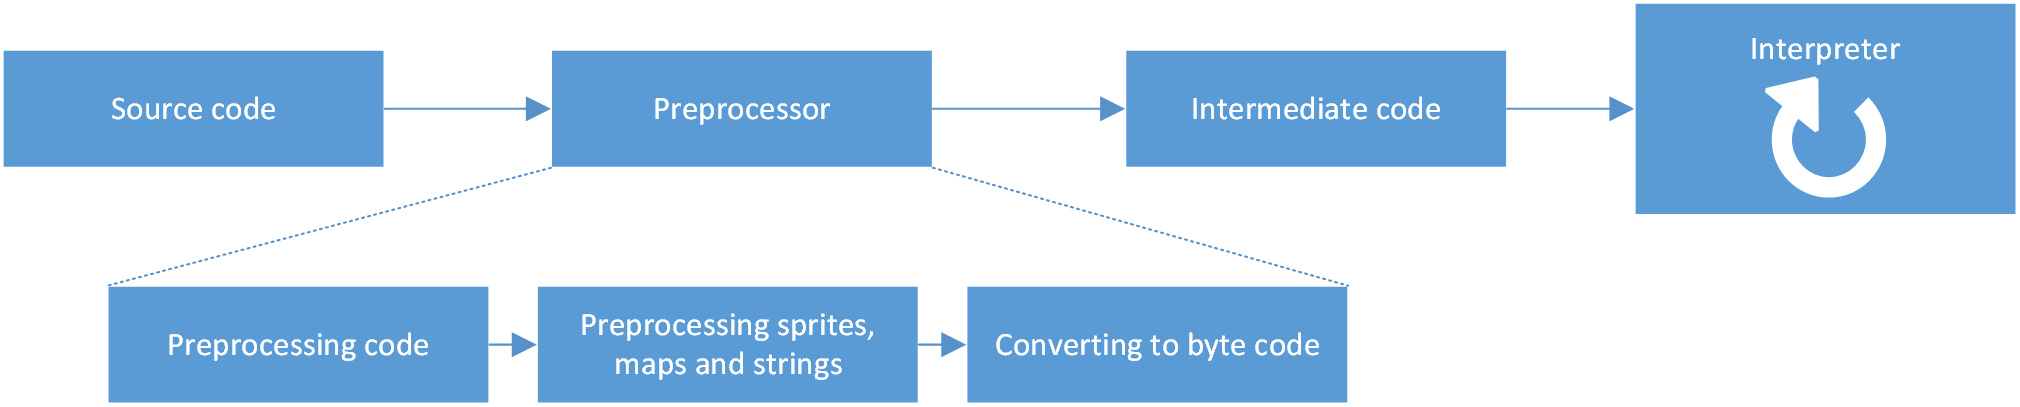
\includegraphics[width=13cm]{InterpreterWorking}
    \caption{LUMEN Interpreter chain}\par
    \label{fig:InterpreterWorking}
\end{figure}

  \chapter{Functions}
\section{Interpreter controller}
\label{cha:InstructionSet}
\begin{table}[H]
\begin {tabularx} {\textwidth} {l|X} Mnemonic (opcode) &  NOP  (0x00)\bigskip\\
\hline
\hline
Function header & inline void ip\textunderscore nop()\bigskip\\
Summary &  This function has exceptionally well performance at doing nothing \bigskip\\
Used by &
\textbf{Interpreter.c}\bigskip \\
\hline
\end{tabularx}
\end{table}
\begin{table}[H]
\begin {tabularx} {\textwidth} {l|X} Mnemonic (opcode) &  LD  (0x01)\bigskip\\
\hline
\hline
Function header & inline void ip\textunderscore load(unsigned char address, unsigned char value)\bigskip\\
Summary &  Loads a fixed value into a specific register. \bigskip\\
Parameters &
\nextitem \textbf{address:}  The address parameter requires an unsigned short containing an 8 bit address.
\nextitem \textbf{value:}  The value parameter requires an unsigned short containing an 8 bit value.
\bigskip \\
Used by &
\textbf{Interpreter.c}\bigskip \\
\hline
\end{tabularx}
\end{table}
\begin{table}[H]
\begin {tabularx} {\textwidth} {l|X} Mnemonic (opcode) &  CPY  (0x02)\bigskip\\
\hline
\hline
Function header & inline void ip\textunderscore copy(unsigned char destaddr, unsigned char srcaddr)\bigskip\\
Summary &  Copies te value from a register to another register. The value in the source register is retained. \bigskip\\
Parameters &
\nextitem \textbf{destaddr:}  The destaddr parameter requires an unsigned short containing an 8 bit address.
\nextitem \textbf{srcaddr:}  The srcaddr parameter requires an unsigned short containing an 8 bit address.
\bigskip \\
Used by &
\textbf{Interpreter.c}\bigskip \\
\hline
\end{tabularx}
\end{table}
\begin{table}[H]
\begin {tabularx} {\textwidth} {l|X} Mnemonic (opcode) &  ST  (0x03)\bigskip\\
\hline
\hline
Function header & inline void ip\textunderscore store(unsigned char destaddr, unsigned char srcaddr)\bigskip\\
Summary &  Store the value of a register to RAM. \bigskip\\
Parameters &
\nextitem \textbf{destaddr:}  The destaddr parameter requires an unsigned short containing an 8 bit address.
\nextitem \textbf{srcaddr:}  The srcaddr parameter requires an unsigned short containing an 8 bit address.
\bigskip \\
Used by &
\textbf{Interpreter.c}\bigskip \\
\hline
\end{tabularx}
\end{table}
\begin{table}[H]
\begin {tabularx} {\textwidth} {l|X} Mnemonic (opcode) &  STI  (0x04)\bigskip\\
\hline
\hline
Function header & inline void ip\textunderscore storeImmediate(unsigned char address, unsigned char value)\bigskip\\
Summary &  Store a fixed value to RAM. \bigskip\\
Parameters &
\nextitem \textbf{address:}  The address parameter requires an unsigned short containing an 8 bit address.
\nextitem \textbf{value:}  The value parameter requires an unsigned short containing an 8 bit value.
\bigskip \\
Used by &
\textbf{Interpreter.c}\bigskip \\
\hline
\end{tabularx}
\end{table}
\begin{table}[H]
\begin {tabularx} {\textwidth} {l|X} Mnemonic (opcode) &  LDR  (0x05)\bigskip\\
\hline
\hline
Function header & inline void ip\textunderscore loadRam(unsigned char destaddr, unsigned char srcaddr)\bigskip\\
Summary &  Load a value from RAM into a register. \bigskip\\
Parameters &
\nextitem \textbf{destaddr:}  The destaddr parameter requires an unsigned short containing an 8 bit address.
\nextitem \textbf{srcaddr:}  The srcaddr parameter requires an unsigned short containing an 8 bit address.
\bigskip \\
Used by &
\textbf{Interpreter.c}\bigskip \\
\hline
\end{tabularx}
\end{table}
\begin{table}[H]
\begin {tabularx} {\textwidth} {l|X} Mnemonic (opcode) &  CMP  (0x06)\bigskip\\
\hline
\hline
Function header & inline void ip\textunderscore compare(unsigned char firstaddress, unsigned char secondaddress)\bigskip\\
Summary &  Compare two values of registers. Two results are possible: 0 means not equal, not 0 means equal. \bigskip\\
Parameters &
\nextitem \textbf{firstaddress:}  The firstaddress parameter requires an unsigned short containing an 8 bit address.
\nextitem \textbf{secondaddress:}  The secondaddress parameter requires an unsigned short containing an 8 bit address.
\bigskip \\
Used by &
\textbf{Interpreter.c}\bigskip \\
\hline
\end{tabularx}
\end{table}
\begin{table}[H]
\begin {tabularx} {\textwidth} {l|X} Mnemonic (opcode) &  GT  (0x07)\bigskip\\
\hline
\hline
Function header & inline void ip\textunderscore greaterThan(unsigned char firstaddress, unsigned char secondaddress)\bigskip\\
Summary &  Check if the first register's value is greater than the second register's value. Two results are possible: 0 means register 2's value is bigger, not 0 means register 1's value is bigger. \bigskip\\
Parameters &
\nextitem \textbf{firstaddress:}  The firstaddress parameter requires an unsigned short containing an 8 bit address.
\nextitem \textbf{secondaddress:}  The secondaddress parameter requires an unsigned short containing an 8 bit address.
\bigskip \\
Used by &
\textbf{Interpreter.c}\bigskip \\
\hline
\end{tabularx}
\end{table}
\begin{table}[H]
\begin {tabularx} {\textwidth} {l|X} Mnemonic (opcode) &  GTI  (0x08)\bigskip\\
\hline
\hline
Function header & inline void ip\textunderscore greaterThanImmediate(unsigned char address, unsigned char value)\bigskip\\
Summary &  Check if a register value is greater than a fixed value Two results are possible: 0 means the fixed value value is bigger, not 0 means the register's value is bigger. \bigskip\\
Parameters &
\nextitem \textbf{address:}  The address parameter requires an unsigned short containing an 8 bit address.
\nextitem \textbf{value:}  The value parameter requires an unsigned short containing an 8 bit value.
\bigskip \\
Used by &
\textbf{Interpreter.c}\bigskip \\
\hline
\end{tabularx}
\end{table}
\begin{table}[H]
\begin {tabularx} {\textwidth} {l|X} Mnemonic (opcode) &  LT  (0x09)\bigskip\\
\hline
\hline
Function header & inline void ip\textunderscore lessThan(unsigned char firstaddress, unsigned char secondaddress)\bigskip\\
Summary &  Check if the first register's value is smaller than the second register's value. Two results are possible: 0 means register 2's value is smaller, not 0 means register 1's value is smaller. \bigskip\\
Parameters &
\nextitem \textbf{firstaddress:}  The firstaddress parameter requires an unsigned short containing an 8 bit address.
\nextitem \textbf{secondaddress:}  The secondaddress parameter requires an unsigned short containing an 8 bit address.
\bigskip \\
Used by &
\textbf{Interpreter.c}\bigskip \\
\hline
\end{tabularx}
\end{table}
\begin{table}[H]
\begin {tabularx} {\textwidth} {l|X} Mnemonic (opcode) &  LTI  (0x0A)\bigskip\\
\hline
\hline
Function header & inline void ip\textunderscore lessThanImmediate(unsigned char address, unsigned char value)\bigskip\\
Summary &  Check if a register value is smaller than a fixed value. Two results are possible: 0 means the fixed value is smaller, not 0 means the register's value is smaller. \bigskip\\
Parameters &
\nextitem \textbf{address:}  The address parameter requires an unsigned short containing an 8 bit address.
\nextitem \textbf{value:}  The value parameter requires an unsigned short containing an 8 bit value.
\bigskip \\
Used by &
\textbf{Interpreter.c}\bigskip \\
\hline
\end{tabularx}
\end{table}
\begin{table}[H]
\begin {tabularx} {\textwidth} {l|X} Mnemonic (opcode) &  SWAP  (0x0B)\bigskip\\
\hline
\hline
Function header & inline void ip\textunderscore swap(unsigned char firstaddress, unsigned char secondaddress)\bigskip\\
Summary &  Swap the values of two registers. Each register gets the value of the other register in one instruction. \bigskip\\
Parameters &
\nextitem \textbf{firstaddress:}  The firstaddress parameter requires an unsigned short containing an 8 bit address.
\nextitem \textbf{secondaddress:}  The secondaddress parameter requires an unsigned short containing an 8 bit address.
\bigskip \\
Used by &
\textbf{Interpreter.c}\bigskip \\
\hline
\end{tabularx}
\end{table}
\begin{table}[H]
\begin {tabularx} {\textwidth} {l|X} Mnemonic (opcode) &  SWAPR  (0x0C)\bigskip\\
\hline
\hline
Function header & inline void ip\textunderscore swapRam(unsigned char firstaddress, unsigned char secondaddress)\bigskip\\
Summary &  Swap the values of two RAM addresses. Each RAM address gets the value of the other RAM address in one instruction. \bigskip\\
Parameters &
\nextitem \textbf{firstaddress:}  The firstaddress parameter requires an unsigned short containing an 8 bit address.
\nextitem \textbf{secondaddress:}  The secondaddress parameter requires an unsigned short containing an 8 bit address.
\bigskip \\
Used by &
\textbf{Interpreter.c}\bigskip \\
\hline
\end{tabularx}
\end{table}
\begin{table}[H]
\begin {tabularx} {\textwidth} {l|X} Mnemonic (opcode) &  ADD  (0x0D)\bigskip\\
\hline
\hline
Function header & inline void ip\textunderscore add(unsigned char firstaddress, unsigned char secondaddress)\bigskip\\
Summary &  Add the values of two registers. The result is stored in the first register. \bigskip\\
Parameters &
\nextitem \textbf{firstaddress:}  The firstaddress parameter requires an unsigned short containing an 8 bit address.
\nextitem \textbf{secondaddress:}  The secondaddress parameter requires an unsigned short containing an 8 bit address.
\bigskip \\
Used by &
\textbf{Interpreter.c}\bigskip \\
\hline
\end{tabularx}
\end{table}
\begin{table}[H]
\begin {tabularx} {\textwidth} {l|X} Mnemonic (opcode) &  ADDI  (0x0E)\bigskip\\
\hline
\hline
Function header & inline void ip\textunderscore addImmediate(unsigned char address, unsigned char value)\bigskip\\
Summary &  Add a fixed value to the value of a register. The result is stored in the register. \bigskip\\
Parameters &
\nextitem \textbf{address:}  The address parameter requires an unsigned short containing an 8 bit address.
\nextitem \textbf{value:}  The value parameter requires an unsigned short containing an 8 bit value.
\bigskip \\
Used by &
\textbf{Interpreter.c}\bigskip \\
\hline
\end{tabularx}
\end{table}
\begin{table}[H]
\begin {tabularx} {\textwidth} {l|X} Mnemonic (opcode) &  SUB  (0x0F)\bigskip\\
\hline
\hline
Function header & inline void ip\textunderscore subtract(unsigned char firstaddress, unsigned char secondaddress)\bigskip\\
Summary &  Subtract the values of two registers. The result is stored in the first register. \bigskip\\
Parameters &
\nextitem \textbf{firstaddress:}  The firstaddress parameter requires an unsigned short containing an 8 bit address.
\nextitem \textbf{secondaddress:}  The secondaddress parameter requires an unsigned short containing an 8 bit address.
\bigskip \\
Used by &
\textbf{Interpreter.c}\bigskip \\
\hline
\end{tabularx}
\end{table}
\begin{table}[H]
\begin {tabularx} {\textwidth} {l|X} Mnemonic (opcode) &  SUBI  (0x10)\bigskip\\
\hline
\hline
Function header & inline void ip\textunderscore subtractImmediate(unsigned char address, unsigned char value)\bigskip\\
Summary &  Subtract a fixed value from the value of a register. The result is stored in the register. \bigskip\\
Parameters &
\nextitem \textbf{address:}  The address parameter requires an unsigned short containing an 8 bit address.
\nextitem \textbf{value:}  The value parameter requires an unsigned short containing an 8 bit value.
\bigskip \\
Used by &
\textbf{Interpreter.c}\bigskip \\
\hline
\end{tabularx}
\end{table}
\begin{table}[H]
\begin {tabularx} {\textwidth} {l|X} Mnemonic (opcode) &  MUL  (0x11)\bigskip\\
\hline
\hline
Function header & inline void ip\textunderscore multiply(unsigned char firstaddress, unsigned char secondaddress)\bigskip\\
Summary &  Multiply the values of two registers. The result is stored in the first register. \bigskip\\
Parameters &
\nextitem \textbf{firstaddress:}  The firstaddress parameter requires an unsigned short containing an 8 bit address.
\nextitem \textbf{secondaddress:}  The secondaddress parameter requires an unsigned short containing an 8 bit address.
\bigskip \\
Used by &
\textbf{Interpreter.c}\bigskip \\
\hline
\end{tabularx}
\end{table}
\begin{table}[H]
\begin {tabularx} {\textwidth} {l|X} Mnemonic (opcode) &  MULI  (0x12)\bigskip\\
\hline
\hline
Function header & inline void ip\textunderscore multiplyImmediate(unsigned char address, unsigned char value)\bigskip\\
Summary &  Multiply a fixed value with the value of a register. The result is stored in the register. \bigskip\\
Parameters &
\nextitem \textbf{address:}  The address parameter requires an unsigned short containing an 8 bit address.
\nextitem \textbf{value:}  The value parameter requires an unsigned short containing an 8 bit value.
\bigskip \\
Used by &
\textbf{Interpreter.c}\bigskip \\
\hline
\end{tabularx}
\end{table}
\begin{table}[H]
\begin {tabularx} {\textwidth} {l|X} Mnemonic (opcode) &  DIV  (0x13)\bigskip\\
\hline
\hline
Function header & inline void ip\textunderscore divide(unsigned char firstaddress, unsigned char secondaddress)\bigskip\\
Summary &  Divide the value of the first register by the value of the second register. The result is stored in the first register. \bigskip\\
Parameters &
\nextitem \textbf{firstaddress:}  The firstaddress parameter requires an unsigned short containing an 8 bit address.
\nextitem \textbf{secondaddress:}  The secondaddress parameter requires an unsigned short containing an 8 bit address.
\bigskip \\
Used by &
\textbf{Interpreter.c}\bigskip \\
\hline
\end{tabularx}
\end{table}
\begin{table}[H]
\begin {tabularx} {\textwidth} {l|X} Mnemonic (opcode) &  DIVI  (0x14)\bigskip\\
\hline
\hline
Function header & inline void ip\textunderscore divideImmediate(unsigned char address, unsigned char value)\bigskip\\
Summary &  Divide the value of a register by a fixed value. The result is stored in the register. \bigskip\\
Parameters &
\nextitem \textbf{address:}  The address parameter requires an unsigned short containing an 8 bit address.
\nextitem \textbf{value:}  The value parameter requires an unsigned short containing an 8 bit value.
\bigskip \\
Used by &
\textbf{Interpreter.c}\bigskip \\
\hline
\end{tabularx}
\end{table}
\begin{table}[H]
\begin {tabularx} {\textwidth} {l|X} Mnemonic (opcode) &  INC  (0x15)\bigskip\\
\hline
\hline
Function header & inline void ip\textunderscore increment(unsigned char address)\bigskip\\
Summary &  Increment the value of a register by one. The result is stored in the register. \bigskip\\
Parameters &
\nextitem \textbf{address:}  The address parameter requires an unsigned short containing an 8 bit address.
\bigskip \\
Used by &
\textbf{Interpreter.c}\bigskip \\
\hline
\end{tabularx}
\end{table}
\begin{table}[H]
\begin {tabularx} {\textwidth} {l|X} Mnemonic (opcode) &  DEC  (0x16)\bigskip\\
\hline
\hline
Function header & inline void ip\textunderscore decrement(unsigned char address)\bigskip\\
Summary &  Decrement the value of a register by one. The result is stored in the register. \bigskip\\
Parameters &
\nextitem \textbf{address:}  The address parameter requires an unsigned short containing an 8 bit address.
\bigskip \\
Used by &
\textbf{Interpreter.c}\bigskip \\
\hline
\end{tabularx}
\end{table}
\begin{table}[H]
\begin {tabularx} {\textwidth} {l|X} Mnemonic (opcode) &  POW  (0x17)\bigskip\\
\hline
\hline
Function header & inline void ip\textunderscore power(unsigned char destaddr, unsigned char pwraddr)\bigskip\\
Summary &  Calculate the power of the value of a register. The power is the value of a register with the address in the second argument. The result is stored in the first register. \bigskip\\
Parameters &
\nextitem \textbf{destaddr:}  The destaddr parameter requires an unsigned short containing an 8 bit address.
\nextitem \textbf{pwraddr:}  The pwraddr parameter requires an unsigned short containing an 8 bit address.
\bigskip \\
Used by &
\textbf{Interpreter.c}\bigskip \\
\hline
\end{tabularx}
\end{table}
\begin{table}[H]
\begin {tabularx} {\textwidth} {l|X} Mnemonic (opcode) &  POWI  (0x18)\bigskip\\
\hline
\hline
Function header & inline void ip\textunderscore pwrvalImmediate(unsigned char destaddr, unsigned char pwrval)\bigskip\\
Summary &  Calculate the power of the value of a register. The power is a fixed value given as the second argument. The result is stored in the register. \bigskip\\
Parameters &
\nextitem \textbf{destaddr:}  The destaddr parameter requires an unsigned short containing an 8 bit address.
\nextitem \textbf{pwrval:}  The pwrval parameter requires an unsigned short containing an 8 bit value.
\bigskip \\
Used by &
\textbf{Interpreter.c}\bigskip \\
\hline
\end{tabularx}
\end{table}
\begin{table}[H]
\begin {tabularx} {\textwidth} {l|X} Mnemonic (opcode) &  SQRT  (0x19)\bigskip\\
\hline
\hline
Function header & inline void ip\textunderscore squareRoot(unsigned char address)\bigskip\\
Summary &  Calculate the square root of the value of a register. The result is stored in the register. \bigskip\\
Parameters &
\nextitem \textbf{address:}  The address parameter requires an unsigned short containing an 8 bit address.
\bigskip \\
Used by &
\textbf{Interpreter.c}\bigskip \\
\hline
\end{tabularx}
\end{table}
\begin{table}[H]
\begin {tabularx} {\textwidth} {l|X} Mnemonic (opcode) &  LOG2  (0x1A)\bigskip\\
\hline
\hline
Function header & inline void ip\textunderscore log2(unsigned char address)\bigskip\\
Summary &  Calculate the log (base 2) of the value of a register. The result is stored in the register. \bigskip\\
Parameters &
\nextitem \textbf{address:}  The address parameter requires an unsigned short containing an 8 bit address.
\bigskip \\
Used by &
\textbf{Interpreter.c}\bigskip \\
\hline
\end{tabularx}
\end{table}
\begin{table}[H]
\begin {tabularx} {\textwidth} {l|X} Mnemonic (opcode) &  LOG10  (0x1B)\bigskip\\
\hline
\hline
Function header & inline void ip\textunderscore log10(unsigned char address)\bigskip\\
Summary &  Calculate the log (base 10) of the value of a register. The result is stored in the register. \bigskip\\
Parameters &
\nextitem \textbf{address:}  The address parameter requires an unsigned short containing an 8 bit address.
\bigskip \\
Used by &
\textbf{Interpreter.c}\bigskip \\
\hline
\end{tabularx}
\end{table}
\begin{table}[H]
\begin {tabularx} {\textwidth} {l|X} Mnemonic (opcode) &  RND  (0x1C)\bigskip\\
\hline
\hline
Function header & inline void ip\textunderscore rand(unsigned char rangemin, unsigned char rangemax)\bigskip\\
Summary &  Generate a random value in a given range. The value is an unsigned char. The range is defined by the first and the second argument as addresses of registers. \bigskip\\
Parameters &
\nextitem \textbf{rangemin:}  The rangemin parameter requires an unsigned short containing an 8 bit address.
\nextitem \textbf{rangemax:}  The rangemax parameter requires an unsigned short containing an 8 bit address.
\bigskip \\
Used by &
\textbf{Interpreter.c}\bigskip \\
\hline
\end{tabularx}
\end{table}
\begin{table}[H]
\begin {tabularx} {\textwidth} {l|X} Mnemonic (opcode) &  RNDI  (0x1D)\bigskip\\
\hline
\hline
Function header & inline void ip\textunderscore randImmediate(unsigned char rangemin, unsigned char rangemax)\bigskip\\
Summary &  Generate a random value in a given range. The value is an unsigned char. The range is defined by the first and the second argument as fixed values. \bigskip\\
Parameters &
\nextitem \textbf{rangemin:}  The rangemin parameter requires an unsigned short containing an 8 bit value.
\nextitem \textbf{rangemax:}  The rangemax parameter requires an unsigned short containing an 8 bit value.
\bigskip \\
Used by &
\textbf{Interpreter.c}\bigskip \\
\hline
\end{tabularx}
\end{table}
\begin{table}[H]
\begin {tabularx} {\textwidth} {l|X} Mnemonic (opcode) &  AND  (0x1E)\bigskip\\
\hline
\hline
Function header & inline void ip\textunderscore bitwiseAnd(unsigned char firstaddress, unsigned char secondaddress)\bigskip\\
Summary &  Performs a bitwise AND on the values of two registers. The result is stored in the HL register. \bigskip\\
Parameters &
\nextitem \textbf{firstaddress:}  The firstaddress parameter requires an unsigned short containing an 8 bit address.
\nextitem \textbf{secondaddress:}  The secondaddress parameter requires an unsigned short containing an 8 bit address.
\bigskip \\
Used by &
\textbf{Interpreter.c}\bigskip \\
\hline
\end{tabularx}
\end{table}
\begin{table}[H]
\begin {tabularx} {\textwidth} {l|X} Mnemonic (opcode) &  ANDI  (0x1F)\bigskip\\
\hline
\hline
Function header & inline void ip\textunderscore bitwiseAndImmediate(unsigned char address, unsigned char value)\bigskip\\
Summary &  Performs a bitwise AND on the value of a register and a fixed value. The result is stored in the HL register. \bigskip\\
Parameters &
\nextitem \textbf{address:}  The address parameter requires an unsigned short containing an 8 bit address.
\nextitem \textbf{value:}  The value parameter requires an unsigned short containing an 8 bit value.
\bigskip \\
Used by &
\textbf{Interpreter.c}\bigskip \\
\hline
\end{tabularx}
\end{table}
\begin{table}[H]
\begin {tabularx} {\textwidth} {l|X} Mnemonic (opcode) &  OR  (0x20)\bigskip\\
\hline
\hline
Function header & inline void ip\textunderscore bitwiseOr(unsigned char firstaddress, unsigned char secondaddress)\bigskip\\
Summary &  Performs a bitwise OR on the values of two registers. The result is stored in the HL register. \bigskip\\
Parameters &
\nextitem \textbf{firstaddress:}  The firstaddress parameter requires an unsigned short containing an 8 bit address.
\nextitem \textbf{secondaddress:}  The secondaddress parameter requires an unsigned short containing an 8 bit address.
\bigskip \\
Used by &
\textbf{Interpreter.c}\bigskip \\
\hline
\end{tabularx}
\end{table}
\begin{table}[H]
\begin {tabularx} {\textwidth} {l|X} Mnemonic (opcode) &  ORI  (0x21)\bigskip\\
\hline
\hline
Function header & inline void ip\textunderscore bitwiseOrImmediate(unsigned char address, unsigned char value)\bigskip\\
Summary &  Performs a bitwise OR on the value of a register and a fixed value. The result is stored in the HL register. \bigskip\\
Parameters &
\nextitem \textbf{address:}  The address parameter requires an unsigned short containing an 8 bit address.
\nextitem \textbf{value:}  The value parameter requires an unsigned short containing an 8 bit value.
\bigskip \\
Used by &
\textbf{Interpreter.c}\bigskip \\
\hline
\end{tabularx}
\end{table}
\begin{table}[H]
\begin {tabularx} {\textwidth} {l|X} Mnemonic (opcode) &  XOR  (0x22)\bigskip\\
\hline
\hline
Function header & inline void ip\textunderscore bitwiseXor(unsigned char firstaddress, unsigned char secondaddress)\bigskip\\
Summary &  Performs a bitwise XOR on the values of two registers. The result is stored in the HL register. \bigskip\\
Parameters &
\nextitem \textbf{firstaddress:}  The firstaddress parameter requires an unsigned short containing an 8 bit address.
\nextitem \textbf{secondaddress:}  The secondaddress parameter requires an unsigned short containing an 8 bit address.
\bigskip \\
Used by &
\textbf{Interpreter.c}\bigskip \\
\hline
\end{tabularx}
\end{table}
\begin{table}[H]
\begin {tabularx} {\textwidth} {l|X} Mnemonic (opcode) &  XORI  (0x23)\bigskip\\
\hline
\hline
Function header & inline void ip\textunderscore bitwiseXorImmediate(unsigned char address, unsigned char value)\bigskip\\
Summary &  Performs a bitwise XOR on the value of a register and a fixed value. The result is stored in the HL register. \bigskip\\
Parameters &
\nextitem \textbf{address:}  The address parameter requires an unsigned short containing an 8 bit address.
\nextitem \textbf{value:}  The value parameter requires an unsigned short containing an 8 bit value.
\bigskip \\
Used by &
\textbf{Interpreter.c}\bigskip \\
\hline
\end{tabularx}
\end{table}
\begin{table}[H]
\begin {tabularx} {\textwidth} {l|X} Mnemonic (opcode) &  NOT  (0x24)\bigskip\\
\hline
\hline
Function header & inline void ip\textunderscore bitwiseNot(unsigned char address)\bigskip\\
Summary &  Performs a bitwise NOT of the value of a registers. The result is stored in the HL register. \bigskip\\
Parameters &
\nextitem \textbf{address:}  The address parameter requires an unsigned short containing an 8 bit address.
\bigskip \\
Used by &
\textbf{Interpreter.c}\bigskip \\
\hline
\end{tabularx}
\end{table}
\begin{table}[H]
\begin {tabularx} {\textwidth} {l|X} Mnemonic (opcode) &  SBIT  (0x25)\bigskip\\
\hline
\hline
Function header & inline void ip\textunderscore setBit(unsigned char address, unsigned char position)\bigskip\\
Summary &  Sets a bit in a register's value, sepcified by the second argument. \bigskip\\
Parameters &
\nextitem \textbf{address:}  The address parameter requires an unsigned short containing an 8 bit address.
\nextitem \textbf{position:}  The position parameter requires an unsigned short containing an 8 bit value.
\bigskip \\
Used by &
\textbf{Interpreter.c}\bigskip \\
\hline
\end{tabularx}
\end{table}
\begin{table}[H]
\begin {tabularx} {\textwidth} {l|X} Mnemonic (opcode) &  CBIT  (0x26)\bigskip\\
\hline
\hline
Function header & inline void ip\textunderscore clearBit(unsigned char address, unsigned char position)\bigskip\\
Summary &  Clears a bit in a register's value, sepcified by the second argument. \bigskip\\
Parameters &
\nextitem \textbf{address:}  The address parameter requires an unsigned short containing an 8 bit address.
\nextitem \textbf{position:}  The position parameter requires an unsigned short containing an 8 bit value.
\bigskip \\
Used by &
\textbf{Interpreter.c}\bigskip \\
\hline
\end{tabularx}
\end{table}
\begin{table}[H]
\begin {tabularx} {\textwidth} {l|X} Mnemonic (opcode) &  JMP  (0x27)\bigskip\\
\hline
\hline
Function header & inline void ip\textunderscore jump(unsigned short address)\bigskip\\
Summary &  Jumps inconditionally to the instruction address specified in the first argument. \bigskip\\
Parameters &
\nextitem \textbf{address:}  The address parameter requires an unsigned short containing a 16 bit address.
\bigskip \\
Used by &
\textbf{Interpreter.c}\bigskip \\
\hline
\end{tabularx}
\end{table}
\begin{table}[H]
\begin {tabularx} {\textwidth} {l|X} Mnemonic (opcode) &  JMPR  (0x28)\bigskip\\
\hline
\hline
Function header & inline void ip\textunderscore jumpRelative(unsigned short address)\bigskip\\
Summary &  Jumps inconditionally by incrementing the program counter with the value of the first argument. If the the program counter overflows, execution of the program is aborted. \bigskip\\
Parameters &
\nextitem \textbf{address:}  The address parameter requires an unsigned short containing a 16 bit address.
\bigskip \\
Used by &
\textbf{Interpreter.c}\bigskip \\
\hline
\end{tabularx}
\end{table}
\begin{table}[H]
\begin {tabularx} {\textwidth} {l|X} Mnemonic (opcode) &  JMPZ  (0x29)\bigskip\\
\hline
\hline
Function header & inline void ip\textunderscore jumpIfZero(unsigned short address)\bigskip\\
Summary &  Jumps if the HL register's value equals zero to the instruction address specified in the first argument. \bigskip\\
Parameters &
\nextitem \textbf{address:}  The address parameter requires an unsigned short containing a 16 bit address.
\bigskip \\
Used by &
\textbf{Interpreter.c}\bigskip \\
\hline
\end{tabularx}
\end{table}
\begin{table}[H]
\begin {tabularx} {\textwidth} {l|X} Mnemonic (opcode) &  JMPRZ  (0x2A)\bigskip\\
\hline
\hline
Function header & inline void ip\textunderscore jumpRelativeIfZero(unsigned short address)\bigskip\\
Summary &  Jumps if the HL register's value equals zero by incrementing the program counter with the value of the first argument. If the the program counter overflows, execution of the program is aborted. \bigskip\\
Parameters &
\nextitem \textbf{address:}  The address parameter requires an unsigned short containing a 16 bit address.
\bigskip \\
Used by &
\textbf{Interpreter.c}\bigskip \\
\hline
\end{tabularx}
\end{table}
\begin{table}[H]
\begin {tabularx} {\textwidth} {l|X} Mnemonic (opcode) &  JMPNZ  (0x2B)\bigskip\\
\hline
\hline
Function header & inline void ip\textunderscore jumpIfNotZero(unsigned short address)\bigskip\\
Summary &  Jumps if the HL register's value does not equal zero to the instruction address specified in the first argument. \bigskip\\
Parameters &
\nextitem \textbf{address:}  The address parameter requires an unsigned short containing a 16 bit address.
\bigskip \\
Used by &
\textbf{Interpreter.c}\bigskip \\
\hline
\end{tabularx}
\end{table}
\begin{table}[H]
\begin {tabularx} {\textwidth} {l|X} Mnemonic (opcode) &  JMPRNZ  (0x2C)\bigskip\\
\hline
\hline
Function header & inline void ip\textunderscore jumpRelativeIfNotZero(unsigned short address)\bigskip\\
Summary &  Jumps if the HL register's value does not equal zero by incrementing the program counter with the value of the first argument. If the the program counter overflows, execution of the program is aborted. \bigskip\\
Parameters &
\nextitem \textbf{address:}  The address parameter requires an unsigned short containing a 16 bit address.
\bigskip \\
Used by &
\textbf{Interpreter.c}\bigskip \\
\hline
\end{tabularx}
\end{table}
\begin{table}[H]
\begin {tabularx} {\textwidth} {l|X} Mnemonic (opcode) &  CALL  (0x2D)\bigskip\\
\hline
\hline
Function header & inline void ip\textunderscore call(unsigned short address)\bigskip\\
Summary &  Executes a subroutine at the address specified in the first argument. Starts by pushing the program counter to the stack. At the end of a subroutine, RET should be called to pop the program counter from the stack and return to the last execution point. If the the program counter overflows, execution of the program is aborted. \bigskip\\
Parameters &
\nextitem \textbf{address:}  The address parameter requires an unsigned short containing a 16 bit address.
\bigskip \\
Used by &
\textbf{Interpreter.c}\bigskip \\
\hline
\end{tabularx}
\end{table}
\begin{table}[H]
\begin {tabularx} {\textwidth} {l|X} Mnemonic (opcode) &  CALLNZ  (0x42)\bigskip\\
\hline
\hline
Function header & inline void ip\textunderscore callIfNotZero(unsigned short address)\bigskip\\
Summary &  Performs a call if and only if the HL register does not contain zero. \bigskip\\
Parameters &
\nextitem \textbf{address:}  The address parameter requires an unsigned short containing a 16 bit address.
\bigskip \\
Used by &
\textbf{Interpreter.c}\bigskip \\
\hline
\end{tabularx}
\end{table}
\begin{table}[H]
\begin {tabularx} {\textwidth} {l|X} Mnemonic (opcode) &  CALLZ  (0x43)\bigskip\\
\hline
\hline
Function header & inline void ip\textunderscore callIfZero(unsigned short address)\bigskip\\
Summary &  Performs a call if and only if the HL register contains zero. \bigskip\\
Parameters &
\nextitem \textbf{address:}  The address parameter requires an unsigned short containing an 8 bit address.
\bigskip \\
Used by &
\textbf{Interpreter.c}\bigskip \\
\hline
\end{tabularx}
\end{table}
\begin{table}[H]
\begin {tabularx} {\textwidth} {l|X} Mnemonic (opcode) &  RET  (0x2E)\bigskip\\
\hline
\hline
Function header & inline void ip\textunderscore ret()\bigskip\\
Summary &  Pops the program counter from the stack and returns to execution after a subroutine was called. \bigskip\\
Used by &
\textbf{Interpreter.c}\bigskip \\
\hline
\end{tabularx}
\end{table}
\begin{table}[H]
\begin {tabularx} {\textwidth} {l|X} Mnemonic (opcode) &  PUSH  (0x2F)\bigskip\\
\hline
\hline
Function header & inline void ip\textunderscore push(unsigned char address)\bigskip\\
Summary &  Pushes a register's value to the stack. \bigskip\\
Parameters &
\nextitem \textbf{address:}  The address parameter requires an unsigned short containing an 8 bit address.
\bigskip \\
Used by &
\textbf{Interpreter.c}\bigskip \\
\hline
\end{tabularx}
\end{table}
\begin{table}[H]
\begin {tabularx} {\textwidth} {l|X} Mnemonic (opcode) &  PUSHI  (0x30)\bigskip\\
\hline
\hline
Function header & inline void ip\textunderscore pushImmediate(unsigned char value)\bigskip\\
Summary &  Pushes a fixed value to the stack. \bigskip\\
Parameters &
\nextitem \textbf{value:}  The value parameter requires an unsigned short containing an 8 bit value.
\bigskip \\
Used by &
\textbf{Interpreter.c}\bigskip \\
\hline
\end{tabularx}
\end{table}
\begin{table}[H]
\begin {tabularx} {\textwidth} {l|X} Mnemonic (opcode) &  POP  (0x31)\bigskip\\
\hline
\hline
Function header & inline void ip\textunderscore pop(unsigned char address)\bigskip\\
Summary &  Pops a value from the stack to a register. \bigskip\\
Parameters &
\nextitem \textbf{address:}  The address parameter requires an unsigned short containing a 8 bit address.
\bigskip \\
Used by &
\textbf{Interpreter.c}\bigskip \\
\hline
\end{tabularx}
\end{table}
\begin{table}[H]
\begin {tabularx} {\textwidth} {l|X} Mnemonic (opcode) &  BRD  (0x32)\bigskip\\
\hline
\hline
Function header & inline void ip\textunderscore buttonRead(unsigned char id)\bigskip\\
Summary &  Reads a controller and places the input in the HL register. The id as the first argument is either 0 or 1, depending on the controller that is to be read. \bigskip\\
Parameters &
\nextitem \textbf{id:}  The id parameter requires an unsigned short containing a 8 bit id.
\bigskip \\
Used by &
\textbf{Interpreter.c}\bigskip \\
\hline
\end{tabularx}
\end{table}
\begin{table}[H]
\begin {tabularx} {\textwidth} {l|X} Mnemonic (opcode) &  BRDS  (0x33)\bigskip\\
\hline
\hline
Function header & inline void ip\textunderscore buttonReadSingle(unsigned char id, unsigned char btn)\bigskip\\
Summary &  Reads a controller and places the input of a specific button in the HL register. If the button is pressed, 1 is placed in HL, else 0. The id as the first argument is either 0 or 1, depending on the controller that is to be read. The button as the second argument is the button that is to be read, for more info, see the controller chapter. \bigskip\\
Parameters &
\nextitem \textbf{id:}  The id parameter requires an unsigned short containing a 8 bit id.
\nextitem \textbf{btn:}  The btn parameter requires an unsigned short containing a 8 bit button id.
\bigskip \\
Used by &
\textbf{Interpreter.c}\bigskip \\
\hline
\end{tabularx}
\end{table}
\begin{table}[H]
\begin {tabularx} {\textwidth} {l|X} Mnemonic (opcode) &  WAITF  (0x34)\bigskip\\
\hline
\hline
Function header & inline void ip\textunderscore waitFor(unsigned char id, unsigned char btn)\bigskip\\
Summary &  Pauses execution of a program until a specific button or buttoncombination is pressed. As long as the buttoncombination does not equal the given one, the program halts. \bigskip\\
Parameters &
\nextitem \textbf{id:}  The id parameter requires an unsigned short containing a 8 bit id.
\nextitem \textbf{btn:}  The btn parameter requires an unsigned short containing a 8 bit button id.
\bigskip \\
Used by &
\textbf{Interpreter.c}\bigskip \\
\hline
\end{tabularx}
\end{table}
\begin{table}[H]
\begin {tabularx} {\textwidth} {l|X} Mnemonic (opcode) &  SCRH  (0x35)\bigskip\\
\hline
\hline
Function header & inline void ip\textunderscore screenHeight()\bigskip\\
Summary &  Places the screenheight in the HL register. \bigskip\\
Used by &
\textbf{Interpreter.c}\bigskip \\
\hline
\end{tabularx}
\end{table}
\begin{table}[H]
\begin {tabularx} {\textwidth} {l|X} Mnemonic (opcode) &  SCRW  (0x36)\bigskip\\
\hline
\hline
Function header & inline void ip\textunderscore screenWidth()\bigskip\\
Summary &  Places the screenwidth in the HL register. \bigskip\\
Used by &
\textbf{Interpreter.c}\bigskip \\
\hline
\end{tabularx}
\end{table}
\begin{table}[H]
\begin {tabularx} {\textwidth} {l|X} Mnemonic (opcode) &  SSPR  (0x37)\bigskip\\
\hline
\hline
Function header & inline void ip\textunderscore setSprite(unsigned char index, unsigned char indexonscreen)\bigskip\\
Summary &  Places a sprite from code to VRAM. The first argument is the index in the sprite array in code. The second argument is the index in the on-screen sprite array. \bigskip\\
Parameters &
\nextitem \textbf{index:}  The index parameter requires an unsigned short containing a 8 bit index.
\nextitem \textbf{indexonscreen:}  The indexonscreen parameter requires an unsigned short containing a 8 bit index.
\bigskip \\
Used by &
\textbf{Interpreter.c}\bigskip \\
\hline
\end{tabularx}
\end{table}
\begin{table}[H]
\begin {tabularx} {\textwidth} {l|X} Mnemonic (opcode) &  USPR  (0x38)\bigskip\\
\hline
\hline
Function header & inline void ip\textunderscore updateSprite(unsigned char indexonscreen, unsigned char x, unsigned char y)\bigskip\\
Summary &  Updates the position of the sprite on the screen. Positioning the sprite out of the bounds of the screen makes the sprite invisible. The second and third argument contain respectively the register with the x position and the y position. \bigskip\\
Parameters &
\nextitem \textbf{indexonscreen:}  The indexonscreen parameter requires an unsigned short containing a 8 bit index.
\nextitem \textbf{x:}  The x parameter requires an unsigned short containing a 8 bit address.
\nextitem \textbf{y:}  The y parameter requires an unsigned short containing a 8 bit address.
\bigskip \\
Used by &
\textbf{Interpreter.c}\bigskip \\
\hline
\end{tabularx}
\end{table}
\begin{table}[H]
\begin {tabularx} {\textwidth} {l|X} Mnemonic (opcode) &  USPRI  (0x4A)\bigskip\\
\hline
\hline
Function header & inline void ip\textunderscore updateSpriteImmediate(unsigned char indexonscreen, unsigned char x, unsigned char y)\bigskip\\
Summary &  Updates the position of the sprite on the screen. Positioning the sprite out of the bounds of the screen makes the sprite invisible. The second and third argument contain respectively the x position and the y position. \bigskip\\
Parameters &
\nextitem \textbf{indexonscreen:}  The indexonscreen parameter requires an unsigned short containing a 8 bit index.
\nextitem \textbf{x:}  The x parameter requires an unsigned short containing a 8 bit value.
\nextitem \textbf{y:}  The y parameter requires an unsigned short containing a 8 bit value.
\bigskip \\
Used by &
\textbf{Interpreter.c}\bigskip \\
\hline
\end{tabularx}
\end{table}
\begin{table}[H]
\begin {tabularx} {\textwidth} {l|X} Mnemonic (opcode) &  CSPR  (0x39)\bigskip\\
\hline
\hline
Function header & inline void ip\textunderscore clearSprite(unsigned char indexonscreen)\bigskip\\
Summary &  Removes a sprite from the onscreen sprite index. \bigskip\\
Parameters &
\nextitem \textbf{indexonscreen:}  The indexonscreen parameter requires an unsigned short containing a 8 bit index.
\bigskip \\
Used by &
\textbf{Interpreter.c}\bigskip \\
\hline
\end{tabularx}
\end{table}
\begin{table}[H]
\begin {tabularx} {\textwidth} {l|X} Mnemonic (opcode) &  SPRX  (0x3A)\bigskip\\
\hline
\hline
Function header & inline void ip\textunderscore checkSpriteX(unsigned char firstindexonscreen, unsigned char secondindexonscreen)\bigskip\\
Summary &  Calculates the horizontal distance between two sprites. The distance (in pixels) is placed in the HL register. \bigskip\\
Parameters &
\nextitem \textbf{firstindexonscreen:}  The firstindexonscreen parameter requires an unsigned short containing a 8 bit index.
\nextitem \textbf{secondindexonscreen:}  The secondindexonscreen parameter requires an unsigned short containing a 8 bit index.
\bigskip \\
Used by &
\textbf{Interpreter.c}\bigskip \\
\hline
\end{tabularx}
\end{table}
\begin{table}[H]
\begin {tabularx} {\textwidth} {l|X} Mnemonic (opcode) &  SPRY  (0x3B)\bigskip\\
\hline
\hline
Function header & inline void ip\textunderscore checkSpriteY(unsigned char firstindexonscreen, unsigned char secondindexonscreen)\bigskip\\
Summary &  Calculates the vertical distance between two sprites. The distance (in pixels) is placed in the HL register. \bigskip\\
Parameters &
\nextitem \textbf{firstindexonscreen:}  The firstindexonscreen parameter requires an unsigned short containing a 8 bit index.
\nextitem \textbf{secondindexonscreen:}  The secondindexonscreen parameter requires an unsigned short containing a 8 bit index.
\bigskip \\
Used by &
\textbf{Interpreter.c}\bigskip \\
\hline
\end{tabularx}
\end{table}
\begin{table}[H]
\begin {tabularx} {\textwidth} {l|X} Mnemonic (opcode) &  SMAP  (0x3C)\bigskip\\
\hline
\hline
Function header & inline void ip\textunderscore setMap(unsigned char index)\bigskip\\
Summary &  Draws a map on the screen. The first argument is the index of the map in the map memory. \bigskip\\
Parameters &
\nextitem \textbf{index:}  The index parameter requires an unsigned short containing a 8 bit index.
\bigskip \\
Used by &
\textbf{Interpreter.c}\bigskip \\
\hline
\end{tabularx}
\end{table}
\begin{table}[H]
\begin {tabularx} {\textwidth} {l|X} Mnemonic (opcode) &  SSTR  (0x3D)\bigskip\\
\hline
\hline
Function header & inline void ip\textunderscore setString(unsigned char index, unsigned char x, unsigned char y)\bigskip\\
Summary &  Draws a string on the screen at a specified position. The first argument is the index of the string in the string memory. \bigskip\\
Parameters &
\nextitem \textbf{index:}  The index parameter requires an unsigned short containing a 8 bit index.
\nextitem \textbf{x:}  The x parameter requires an unsigned short containing a 8 bit value.
\nextitem \textbf{y:}  The y parameter requires an unsigned short containing a 8 bit value.
\bigskip \\
Used by &
\textbf{Interpreter.c}\bigskip \\
\hline
\end{tabularx}
\end{table}
\begin{table}[H]
\begin {tabularx} {\textwidth} {l|X} Mnemonic (opcode) &  DLY  (0x3E)\bigskip\\
\hline
\hline
Function header & inline void ip\textunderscore delay(unsigned char index)\bigskip\\
Summary &  Waits for an amount of milliseconds equal to the value of the register given in the first argument. \bigskip\\
Parameters &
\nextitem \textbf{index:}  The index parameter requires an unsigned short containing a 8 bit index.
\bigskip \\
Used by &
\textbf{Interpreter.c}\bigskip \\
\hline
\end{tabularx}
\end{table}
\begin{table}[H]
\begin {tabularx} {\textwidth} {l|X} Mnemonic (opcode) &  DLYI  (0x3F)\bigskip\\
\hline
\hline
Function header & inline void ip\textunderscore delayImmediate(unsigned char value)\bigskip\\
Summary &  Waits for an amount of milliseconds equal to the fixed value given in the first argument. \bigskip\\
Parameters &
\nextitem \textbf{value:}  The value parameter requires an unsigned short containing a 8 bit value.
\bigskip \\
Used by &
\textbf{Interpreter.c}\bigskip \\
\hline
\end{tabularx}
\end{table}
\begin{table}[H]
\begin {tabularx} {\textwidth} {l|X} Mnemonic (opcode) &  CTMR  (0x40)\bigskip\\
\hline
\hline
Function header & inline void ip\textunderscore clearTimer()\bigskip\\
Summary &  Clears the timer by resetting its value to zero. \bigskip\\
Used by &
\textbf{Interpreter.c}\bigskip \\
\hline
\end{tabularx}
\end{table}
\begin{table}[H]
\begin {tabularx} {\textwidth} {l|X} Mnemonic (opcode) &  RTMR  (0x41)\bigskip\\
\hline
\hline
Function header & inline void ip\textunderscore readTimer()\bigskip\\
Summary &  Places the value of the timer in the HL register. \bigskip\\
Used by &
\textbf{Interpreter.c}\bigskip \\
\hline
\end{tabularx}
\end{table}
\begin{table}[H]
\begin {tabularx} {\textwidth} {l|X} Mnemonic (opcode) &  DON  (0x44)\bigskip\\
\hline
\hline
Function header & inline void allOn()\bigskip\\
Summary &  Sets all pixels on the screen to the on-state. The actual framebuffer is not affected. To get back to drawing the buffer, call normalMode(). No redraw is needed to change the state. \bigskip\\
Used by &
\textbf{Interpreter.c}\bigskip \\
\hline
\end{tabularx}
\end{table}
\begin{table}[H]
\begin {tabularx} {\textwidth} {l|X} Mnemonic (opcode) &  DOFF  (0x45)\bigskip\\
\hline
\hline
Function header & inline void allOff()\bigskip\\
Summary &  Sets all pixels on the screen to the off-state. The actual framebuffer is not affected. To get back to drawing the buffer, call normalMode(). No redraw is needed to change the state. \bigskip\\
Used by &
\textbf{Interpreter.c}\bigskip \\
\hline
\end{tabularx}
\end{table}
\begin{table}[H]
\begin {tabularx} {\textwidth} {l|X} Mnemonic (opcode) &  DINV  (0x46)\bigskip\\
\hline
\hline
Function header & inline void invertedMode()\bigskip\\
Summary &  Sets the screen to drawing the framebuffer inverted. The actual framebuffer is not affected, nor the operation of its states. A cleared pixel will be lit, and a lit pixel will be cleared on screen. No redraw is needed to change the state. \bigskip\\
Used by &
\textbf{Interpreter.c}\bigskip \\
\hline
\end{tabularx}
\end{table}
\begin{table}[H]
\begin {tabularx} {\textwidth} {l|X} Mnemonic (opcode) &  DNRM  (0x47)\bigskip\\
\hline
\hline
Function header & inline void normalMode()\bigskip\\
Summary &  Sets the screen to drawing the framebuffer. No redraw is needed to change the state. \bigskip\\
Used by &
\textbf{Interpreter.c}\bigskip \\
\hline
\end{tabularx}
\end{table}
\begin{table}[H]
\begin {tabularx} {\textwidth} {l|X} Mnemonic (opcode) &  DRDRW  (0x48)\bigskip\\
\hline
\hline
Function header & inline void redraw()\bigskip\\
Summary &  Redraws the framebuffer to the screen. If allOn or allOff has been called right before a redraw, it is needed to call normalMode to draw the framebuffer. \bigskip\\
Used by &
\textbf{Interpreter.c}\bigskip \\
\hline
\end{tabularx}
\end{table}
\begin{table}[H]
\begin {tabularx} {\textwidth} {l|X} Mnemonic (opcode) &  DCLR  (0x49)\bigskip\\
\hline
\hline
Function header & inline void clearAll()\bigskip\\
Summary &  Clears the entire framebuffer by resetting its pixelvalues to zero. Will only be seen after a redraw. After a clearAll, the framebuffer can be written to immediately to update the screen. \bigskip\\
Used by &
\textbf{Interpreter.c}\bigskip \\
\hline
\end{tabularx}
\end{table}
\begin{table}[H]
\begin {tabularx} {\textwidth} {l|X} Function header & void ip\textunderscore initInterpreter()\bigskip\\
\hline
\hline Summary &  Inits the interpreter by resetting all its properties. This should be called before each ip\textunderscore startInterpreter(). \bigskip\\
Used by &
\textbf{Interpreter.c},  \textbf{Interpreter.h},  \textbf{Main.c}\bigskip \\
\hline
\end{tabularx}
\end{table}
\begin{table}[H]
\begin {tabularx} {\textwidth} {l|X} Function header & void ip\textunderscore startInterpreter()\bigskip\\
\hline
\hline Summary &  Starts the actual interpreter. Before each ip\textunderscore startInterpreter call, ip\textunderscore initInterpreter should be called unless the state of the interpreter is to be saved. To be able to execute code, a RAM module should be attached to the controller containing the code, sprites, maps and strings, carefully mapped to the memory. define DEBUGASSERT at the top to enable assert functions to be used, turned off by default. These asserts can check if a method actually does what it is supposed to do, and can help debugging of written code. \bigskip\\
Used by &
\textbf{Interpreter.c},  \textbf{Interpreter.h},  \textbf{Main.c}\bigskip \\
\hline
\end{tabularx}
\end{table}
\begin{table}[H]
\begin {tabularx} {\textwidth} {l|X} Function header & void io\textunderscore initSlaveSelect()\bigskip\\
\hline
\hline Summary & \bigskip\\
Used by &
\textbf{IOcontrol.c},  \textbf{IOcontrol.h}\bigskip \\
\hline
\end{tabularx}
\end{table}
\begin{table}[H]
\begin {tabularx} {\textwidth} {l|X} Function header & unsigned char io\textunderscore readProgramMemory(unsigned short address)\bigskip\\
\hline
\hline Summary &  This function reads 1 byte of data from the external program RAM chip at a given address. The program RAM contains the program code that is executed by the interpreter. \bigskip\\
Parameters &
\nextitem \textbf{address:}  The address parameter requires an unsigned short containing a 16 bit address. The program address range is from 0x00000 to 0x0FFFF.
\bigskip \\
Returns &  This method returns a unsigned char containing the data that was stored at the given address. \bigskip\\
Used by &
\textbf{IOcontrol.c},  \textbf{IOcontrol.h}\bigskip \\
\hline
\end{tabularx}
\end{table}
\begin{table}[H]
\begin {tabularx} {\textwidth} {l|X} Function header & unsigned char io\textunderscore readDataMemory(unsigned short address)\bigskip\\
\hline
\hline Summary &  This function reads 1 byte of data from the external data RAM chip at a given address. The data RAM contains the sprites, maps, strings, settings and savebanks. \bigskip\\
Parameters &
\nextitem \textbf{address:}  The address parameter requires an unsigned short containing a 16 bit address. The data address range is from 0xF0000 to 0xFFFFF.
\bigskip \\
Returns &  This method returns a unsigned char containing the data that was stored at the given address. \bigskip\\
Used by &
\textbf{IOcontrol.c},  \textbf{IOcontrol.h}\bigskip \\
\hline
\end{tabularx}
\end{table}
\begin{table}[H]
\begin {tabularx} {\textwidth} {l|X} Function header & void io\textunderscore writeToDataMemory(unsigned short address, unsigned char data)\bigskip\\
\hline
\hline Summary &  This function writes 1 byte of data to the external data RAM at a given address. \bigskip\\
Parameters &
\nextitem \textbf{address:}  The address parameter requires an unsigned short containing a 16 bit address. The data address range is from 0xF0000 to 0xFFFFF.
\bigskip \\
Used by &
\textbf{IOcontrol.c},  \textbf{IOcontrol.h}\bigskip \\
\hline
\end{tabularx}
\end{table}
\begin{table}[H]
\begin {tabularx} {\textwidth} {l|X} Function header & unsigned char io\textunderscore readController(unsigned char controllerNumber)\bigskip\\
\hline
\hline Summary &  This function reads the game controller buttons state for a given controller number. \bigskip\\
Parameters &
\nextitem \textbf{ControllerNumber:}  This parameter contains the controller number: Controller1 = 0x00 Controller2 = 0xff
\bigskip \\
Returns &  The method returns a unsigned char containing the controller button state. The meaning of each bit: BIT 0: A BIT 1: B BIT 2: SELECT BIT 3: START BIT 4: DPAD UP BIT 5: DPAD DOWN BIT 6: DPAD LEFT BIT 7: DPAD RIGHT \bigskip\\
Used by &
\textbf{IOcontrol.c},  \textbf{IOcontrol.h}\bigskip \\
\hline
\end{tabularx}
\end{table}
\begin{table}[H]
\begin {tabularx} {\textwidth} {l|X} Function header & void io\textunderscore initIO()\bigskip\\
\hline
\hline Summary &  This function sets up the IOcontrol interface. It performs the following actions: - RAM interface setup - SoftSPI interface setup and slave select initialisation - Loads the sprites into the video memory - Loads the strings into the video memory - Loads the maps into the video memory \bigskip\\
Note &  This function has a long execution time. \bigskip\\
Used by &
\textbf{Interpreter.c},  \textbf{IOcontrol.c},  \textbf{IOcontrol.h},  \textbf{Main.c}\bigskip \\
\hline
\end{tabularx}
\end{table}
\begin{table}[H]
\begin {tabularx} {\textwidth} {l|X} Function header & void io\textunderscore allOn()\bigskip\\
\hline
\hline Summary &  This function lights up all the pixels of the LCD screen without overwriting the video memory. \bigskip\\
Used by &
\textbf{Interpreter.c},  \textbf{IOcontrol.c},  \textbf{IOcontrol.h},  \textbf{Main.c}\bigskip \\
\hline
\end{tabularx}
\end{table}
\begin{table}[H]
\begin {tabularx} {\textwidth} {l|X} Function header & void io\textunderscore allOff()\bigskip\\
\hline
\hline Summary &  This function disables all the pixels of the LCD screen without overwriting the video memory. \bigskip\\
Used by &
\textbf{Interpreter.c},  \textbf{IOcontrol.c},  \textbf{IOcontrol.h},  \textbf{Main.c}\bigskip \\
\hline
\end{tabularx}
\end{table}
\begin{table}[H]
\begin {tabularx} {\textwidth} {l|X} Function header & void io\textunderscore invert()\bigskip\\
\hline
\hline Summary &  This function inverts all the pixels of the LCD screen overwriting the video memory. This means that a black pixel turns white and a white pixel turns into black. \bigskip\\
Used by &
\textbf{Interpreter.c},  \textbf{IOcontrol.c},  \textbf{IOcontrol.h}\bigskip \\
\hline
\end{tabularx}
\end{table}
\begin{table}[H]
\begin {tabularx} {\textwidth} {l|X} Function header & void io\textunderscore setCursor(unsigned char x , unsigned char y)\bigskip\\
\hline
\hline Summary &  This function sets the coordinates of the LCD display in the videobuffer. TOTO: EXPLAIN The coordinate (0,0) is located top left. \bigskip\\
Parameters &
\nextitem \textbf{x:}  This parameter of type unsigned char contains the x-coordinate of the cursor.
\nextitem \textbf{y:}  This parameter of type unsigned char contains the y-coordinate of the cursor.
\bigskip \\
Used by &
\textbf{IOcontrol.h}\bigskip \\
\hline
\end{tabularx}
\end{table}
\begin{table}[H]
\begin {tabularx} {\textwidth} {l|X} Function header & void io\textunderscore updateSprite(unsigned char indexVram,unsigned char x, unsigned char y)\bigskip\\
\hline
\hline Summary &  This function updates the position of a sprite in the video memory. \bigskip\\
Parameters &
\nextitem \textbf{indexVram:}  This parameter of type unsigned char container the index of the sprite in the video RAM.
\nextitem \textbf{x:}  This parameter of type unsigned char contains the x-coordinate of the cursor.
\nextitem \textbf{y:}  This parameter of type unsigned char contains the y-coordinate of the cursor.
\bigskip \\
Used by &
\textbf{Interpreter.c},  \textbf{IOcontrol.c},  \textbf{IOcontrol.h}\bigskip \\
\hline
\end{tabularx}
\end{table}
\begin{table}[H]
\begin {tabularx} {\textwidth} {l|X} Function header & void io\textunderscore setSprite(unsigned char index, unsigned char indexVram)\bigskip\\
\hline
\hline Summary &  This function initialize a sprite in the video memory at a given position. \bigskip\\
Parameters &
\nextitem \textbf{index:}  This parameter of type unsigned char contains the index of the sprite in ROM memory.
\nextitem \textbf{indexVram:}  This parameter of type unsigned char container the index of the sprite in the video RAM.
\nextitem \textbf{x:}  This parameter of type unsigned char contains the x-coordinate of the cursor.
\nextitem \textbf{y:}  This parameter of type unsigned char contains the y-coordinate of the cursor.
\bigskip \\
Used by &
\textbf{Interpreter.c},  \textbf{IOcontrol.c},  \textbf{IOcontrol.h},  \textbf{Main.c}\bigskip \\
\hline
\end{tabularx}
\end{table}
\begin{table}[H]
\begin {tabularx} {\textwidth} {l|X} Function header & void io\textunderscore clearSprite(unsigned char index)\bigskip\\
\hline
\hline Summary &  This function clears a sprite given by the index parameter in the video memory. \bigskip\\
Parameters &
\nextitem \textbf{index:}  This parameter of type unsigned char contains the index of the sprite in ROM memory.
\bigskip \\
Used by &
\textbf{Interpreter.c},  \textbf{IOcontrol.c},  \textbf{IOcontrol.h}\bigskip \\
\hline
\end{tabularx}
\end{table}
\begin{table}[H]
\begin {tabularx} {\textwidth} {l|X} Function header & void io\textunderscore drawString(unsigned char index, unsigned char x, unsigned char y)\bigskip\\
\hline
\hline Summary &  This function draws a string given by the index parameter on the screen at a given position. \bigskip\\
Parameters &
\nextitem \textbf{index:}  This parameter of type unsigned char contains the index of the string in ROM memory.
\nextitem \textbf{x:}  This parameter of type unsigned char contains the x-coordinate of the cursor.
\nextitem \textbf{y:}  This parameter of type unsigned char contains the y-coordinate of the cursor.
\bigskip \\
Used by &
\textbf{Interpreter.c},  \textbf{IOcontrol.c},  \textbf{IOcontrol.h}\bigskip \\
\hline
\end{tabularx}
\end{table}
\begin{table}[H]
\begin {tabularx} {\textwidth} {l|X} Function header & void io\textunderscore drawMap(unsigned char index)\bigskip\\
\hline
\hline Summary &  This function draws a map with a given index on the LCD screen. \bigskip\\
Parameters &
\nextitem \textbf{index:}  This parameter of type unsigned char contains the index of the map in ROM memory.
\bigskip \\
Used by &
\textbf{Interpreter.c},  \textbf{IOcontrol.c},  \textbf{IOcontrol.h}\bigskip \\
\hline
\end{tabularx}
\end{table}
\begin{table}[H]
\begin {tabularx} {\textwidth} {l|X} Function header & void io\textunderscore clearAll()\bigskip\\
\hline
\hline Summary &  This function clears al the elements on the LCD screen. \bigskip\\
Used by &
\textbf{Interpreter.c},  \textbf{IOcontrol.c},  \textbf{IOcontrol.h}\bigskip \\
\hline
\end{tabularx}
\end{table}
\begin{table}[H]
\begin {tabularx} {\textwidth} {l|X} Function header & void io\textunderscore clearStrings()\bigskip\\
\hline
\hline Summary &  This function clears the string buffer. \bigskip\\
Used by &
\textbf{IOcontrol.c},  \textbf{IOcontrol.h}\bigskip \\
\hline
\end{tabularx}
\end{table}
\begin{table}[H]
\begin {tabularx} {\textwidth} {l|X} Function header & void io\textunderscore clearGraphics()\bigskip\\
\hline
\hline Summary &  This function clears the display buffer. \bigskip\\
Used by &
\textbf{IOcontrol.c},  \textbf{IOcontrol.h}\bigskip \\
\hline
\end{tabularx}
\end{table}
\begin{table}[H]
\begin {tabularx} {\textwidth} {l|X} Function header & void io\textunderscore redraw()\bigskip\\
\hline
\hline Summary &  This function redraws the displaybuffer to the LCD screen. \bigskip\\
Used by &
\textbf{Interpreter.c},  \textbf{IOcontrol.c},  \textbf{IOcontrol.h},  \textbf{Main.c}\bigskip \\
\hline
\end{tabularx}
\end{table}
\begin{table}[H]
\begin {tabularx} {\textwidth} {l|X} Function header & void io\textunderscore normalMode()\bigskip\\
\hline
\hline Summary &  This function sets the LCD screen back to normal mode. \bigskip\\
Used by &
\textbf{Interpreter.c},  \textbf{IOcontrol.c},  \textbf{IOcontrol.h}\bigskip \\
\hline
\end{tabularx}
\end{table}
\begin{table}[H]
\begin {tabularx} {\textwidth} {l|X} Function header & void rd\textunderscore initRAM()\bigskip\\
\hline
\hline Summary & \bigskip\\
Used by &
\textbf{IOcontrol.c},  \textbf{RAMdriver.c},  \textbf{RAMdriver.h}\bigskip \\
\hline
\end{tabularx}
\end{table}
\begin{table}[H]
\begin {tabularx} {\textwidth} {l|X} Function header & void rd\textunderscore setBank(unsigned char bank)\bigskip\\
\hline
\hline Summary &  This function selects a memorybank. \bigskip\\
Parameters &
\nextitem \textbf{bank:}  The bank parameter contains the selected bank: PROGMEM = 0, DATAMEM = 1
\bigskip \\
Used by &
\textbf{IOcontrol.c},  \textbf{RAMdriver.c},  \textbf{RAMdriver.h}\bigskip \\
\hline
\end{tabularx}
\end{table}
\begin{table}[H]
\begin {tabularx} {\textwidth} {l|X} Function header & unsigned char rd\textunderscore getBank()\bigskip\\
\hline
\hline Summary &  Function to get the selected bank \bigskip\\
Returns &  The method returns a unsigned char containing the selected bank \bigskip\\
Used by &
\textbf{RAMdriver.c},  \textbf{RAMdriver.h}\bigskip \\
\hline
\end{tabularx}
\end{table}
\begin{table}[H]
\begin {tabularx} {\textwidth} {l|X} Function header & void rd\textunderscore writeToRAM(unsigned short address, unsigned char value)\bigskip\\
\hline
\hline Summary &  Function to write data (1 byte) to the external RAM in a given address \bigskip\\
Parameters &
\nextitem \textbf{address:}  The address parameter requires an 16 bit address (unsigned short)
\nextitem \textbf{value:}  Parameter value is helds the value that needs to be stored in the ROM
\bigskip \\
Used by &
\textbf{IOcontrol.c},  \textbf{RAMdriver.c},  \textbf{RAMdriver.h}\bigskip \\
\hline
\end{tabularx}
\end{table}
\begin{table}[H]
\begin {tabularx} {\textwidth} {l|X} Function header & unsigned char rd\textunderscore readFromRAM(unsigned short address)\bigskip\\
\hline
\hline Summary &  Function the read data (1 byte) from a given address \bigskip\\
Parameters &
\nextitem \textbf{address:}  The address parameter requires an 16 bit address (unsigned short).
\bigskip \\
Returns &  The method returns a unsigned char containing the data in the address \bigskip\\
Used by &
\textbf{RAMdriver.c},  \textbf{RAMdriver.h}\bigskip \\
\hline
\end{tabularx}
\end{table}
\begin{table}[H]
\begin {tabularx} {\textwidth} {l|X} Function header & void ss\textunderscore initSPI()\bigskip\\
\hline
\hline Summary &  Initialisation of the software SPI pins. Sets all the output pins low. Mind the tris register, this has to be set manually! The standard in this case is trisa = 0b00000100 \bigskip\\
Used by &
\textbf{IOcontrol.c},  \textbf{SoftSPIdriver.c},  \textbf{SoftSPIdriver.h}\bigskip \\
\hline
\end{tabularx}
\end{table}
\begin{table}[H]
\begin {tabularx} {\textwidth} {l|X} Function header & void ss\textunderscore sendByte(unsigned char data)\bigskip\\
\hline
\hline Summary &  Sends a byte over SPI to the selected slave. \bigskip\\
Parameters &
\nextitem \textbf{data:}  The data argument is an unsigned char, the byte we want to send.
\bigskip \\
Used by &
\textbf{IOcontrol.c},  \textbf{SoftSPIdriver.c},  \textbf{SoftSPIdriver.h}\bigskip \\
\hline
\end{tabularx}
\end{table}
\begin{table}[H]
\begin {tabularx} {\textwidth} {l|X} Function header & unsigned char ss\textunderscore readByte()\bigskip\\
\hline
\hline Summary &  Reads a byte over SPI from the selected slave. \bigskip\\
Returns &  The method returns an unsigned char, the data received over SPI. \bigskip\\
Used by &
\textbf{SoftSPIdriver.c},  \textbf{SoftSPIdriver.h}\bigskip \\
\hline
\end{tabularx}
\end{table}


\section{Graphics controller}

\subsection{CommandControl.h}
\par This file provides the functions needed for the hardware SPI.
It provides
	- cc\textunderscore initCommandControl()
	- cc\textunderscore spiCallback()
	- cc\textunderscore control()
It requires
	- eventhandler()
	- hs\textunderscore initSPI()
	- hs\textunderscore readByte()
	- gc\textunderscore loadSprite(unsigned char refNumber, unsigned char *data)
	- gc\textunderscore setSprite(unsigned char refNumber, unsigned char listNumber, unsigned char xpos, unsigned char ypos)
	- gc\textunderscore clearSprite(unsigned char listNumber)
	- gc\textunderscore updateSprite(unsigned char listNumber, unsigned char xpos, unsigned char ypos)
	- gc\textunderscore loadMap(unsigned char mapNumber)
	- gc\textunderscore drawMap(unsigned char mapNumber, unsigned char xoffset, unsigned char yoffset)
	- gc\textunderscore loadString(unsigned char stringNumber)
	- gc\textunderscore drawString(unsigned char xpos, unsigned char ypos, unsigned char stringNumber)
	- gc\textunderscore redraw()
	- gc\textunderscore allOn()
	- gc\textunderscore allOff()
	- gc\textunderscore invertedMode()
	- gc\textunderscore normalMode()
	- gc\textunderscore clearAll()
	- gc\textunderscore clearGraphics()
	- gc\textunderscore clearStrings()

\begin{table}[H]
\begin {tabularx} {\textwidth} {l|X} Function header & void cc\textunderscore initCommandControl()\bigskip\\
\hline
\hline Summary & 	This initializes the command control, calls the needed methods to set some registers \bigskip\\
Used by &
 \textbf{CommandControl.c},  \textbf{CommandControl.h},  \textbf{Graphics.c}\bigskip \\
\hline
 \end{tabularx}
 \end{table}
\begin{table}[H]
\begin {tabularx} {\textwidth} {l|X} Function header & void cc\textunderscore spiCallback()\bigskip\\
\hline
\hline Summary & 	Contains the code that must be executed on SPI interrupt This interrupt is triggered on receiving a full byte \bigskip\\
Used by &
 \textbf{CommandControl.c},  \textbf{CommandControl.h},  \textbf{Eventhandler.c}\bigskip \\
\hline
 \end{tabularx}
 \end{table}
\begin{table}[H]
\begin {tabularx} {\textwidth} {l|X} Function header & void cc\textunderscore control()\bigskip\\
\hline
\hline Summary & 	This method does all the command handling It checks the receive buffer and calls the correct middleware methods \bigskip\\
Used by &
 \textbf{CommandControl.c},  \textbf{CommandControl.h},  \textbf{Graphics.c}\bigskip \\
\hline
 \end{tabularx}
 \end{table}

\subsection{GraphicsControl.h}
\par This file provides the functions needed for the hardware SPI.
It provides
	- gc\textunderscore drawPixel(unsigned char xpos, unsigned char ypos, unsigned char color)
	- gc\textunderscore setPixel(unsigned char xpos, unsigned char ypos)
	- gc\textunderscore clearPixel(unsigned char xpos, unsigned char ypos)
	- gc\textunderscore drawByte(unsigned char xpos, unsigned char ypos, unsigned char data)
	- gc\textunderscore testbit(unsigned char data, unsigned char number)
	- gc\textunderscore loadSprite(unsigned char refNumber, unsigned char *data)
	- gc\textunderscore setSprite(unsigned char refNumber, unsigned char listNumber, unsigned char xpos, unsigned char ypos)
	- gc\textunderscore clearSprite(unsigned char listNumber)
	- gc\textunderscore updateSprite(unsigned char listNumber, unsigned char xpos, unsigned char ypos)
	- gc\textunderscore loadMap(unsigned char mapNumber)
	- gc\textunderscore drawMap(unsigned char mapNumber, unsigned char xoffset, unsigned char yoffset)
	- gc\textunderscore loadString(unsigned char stringNumber)
	- gc\textunderscore drawString(unsigned char xpos, unsigned char ypos, unsigned char stringNumber)
	- gc\textunderscore initLCD()
	- gc\textunderscore resetCursor()
	- gc\textunderscore dataMode()
	- gc\textunderscore commandMode()
	- gc\textunderscore sendCommand()
	- gc\textunderscore sendData()
	- gc\textunderscore redraw()
	- gc\textunderscore allOn()
	- gc\textunderscore allOff()
	- gc\textunderscore invertedMode()
	- gc\textunderscore normalMode()
	- gc\textunderscore clearAll()
	- gc\textunderscore clearGraphics()
	- gc\textunderscore clearStrings()
It requires
	- hs\textunderscore readByte()
	- hs\textunderscore dataAvailable()
	- ss\textunderscore initSPI()
	- ss\textunderscore sendByte(unsigned char data)

\begin{table}[H]
\begin {tabularx} {\textwidth} {l|X} Function header & void gc\textunderscore drawPixel(unsigned char xpos, unsigned char ypos, unsigned char color)\bigskip\\
\hline
\hline Summary & 	Draws a pixel with a specified color at a specified location on the screen \bigskip\\
Parameters &
\nextitem \textbf{xpos:}  Unsigned char denoting the x position on the screen
\nextitem \textbf{ypos:}  Unsigned char denoting the y position on the screen
\nextitem \textbf{color:}  Unsigned char denoting the color of the pixel
\bigskip \\
Used by &
 \textbf{GraphicsControl.c},  \textbf{GraphicsControl.h}\bigskip \\
\hline
 \end{tabularx}
 \end{table}
\begin{table}[H]
\begin {tabularx} {\textwidth} {l|X} Function header & void gc\textunderscore setPixel(unsigned char xpos, unsigned char ypos)\bigskip\\
\hline
\hline Summary & 	Draws a pixel with color = 1 at a specified location on the screen \bigskip\\
Parameters &
\nextitem \textbf{xpos:}  Unsigned char denoting the x position on the screen
\nextitem \textbf{ypos:}  Unsigned char denoting the y position on the screen
\bigskip \\
Used by &
 \textbf{GraphicsControl.c},  \textbf{GraphicsControl.h}\bigskip \\
\hline
 \end{tabularx}
 \end{table}
\begin{table}[H]
\begin {tabularx} {\textwidth} {l|X} Function header & void gc\textunderscore clearPixel(unsigned char xpos, unsigned char ypos)\bigskip\\
\hline
\hline Summary & 	Draws a pixel with color = 0 at a specified location on the screen \bigskip\\
Parameters &
\nextitem \textbf{xpos:}  Unsigned char denoting the x position on the screen
\nextitem \textbf{ypos:}  Unsigned char denoting the y position on the screen
\bigskip \\
Used by &
 \textbf{GraphicsControl.c},  \textbf{GraphicsControl.h}\bigskip \\
\hline
 \end{tabularx}
 \end{table}
\begin{table}[H]
\begin {tabularx} {\textwidth} {l|X} Function header & void gc\textunderscore drawByte(unsigned char xpos, unsigned char ypos, unsigned char data)\bigskip\\
\hline
\hline Summary & 	Draws 8 subsequent pixels starting at a specified location on the screen The folowing pixels are each drawn below the previous drawn pixel (ie. advancing in y position) If the end of the screen is reached, the rest of the pixels is not drawn \bigskip\\
Parameters &
\nextitem \textbf{xpos:}  Unsigned char denoting the starting x position on the screen
\nextitem \textbf{ypos:}  Unsigned char denoting the starting y position on the screen
\nextitem \textbf{data:}  Unsigned char containing the pixel data, is used lsb first
\bigskip \\
Used by &
 \textbf{GraphicsControl.c},  \textbf{GraphicsControl.h}\bigskip \\
\hline
 \end{tabularx}
 \end{table}
\begin{table}[H]
\begin {tabularx} {\textwidth} {l|X} Function header & unsigned char gc\textunderscore testbit(unsigned char data, unsigned char number)\bigskip\\
\hline
\hline Summary & 	Test the number bit of a certain byte data \bigskip\\
Parameters &
\nextitem \textbf{data:}  An unsigned char denoting the data byte we want a to test a bit from
\nextitem \textbf{number:}  The nth bit from the data byte we want to test, with nth being equal to number
\bigskip \\
Returns &  Unsigned char, in fact return is restricted to 0 or 1 \bigskip\\
Used by &
 \textbf{GraphicsControl.c},  \textbf{GraphicsControl.h}\bigskip \\
\hline
 \end{tabularx}
 \end{table}
\begin{table}[H]
\begin {tabularx} {\textwidth} {l|X} Function header & void gc\textunderscore loadSprite(unsigned char refNumber, unsigned char *data)\bigskip\\
\hline
\hline Summary & 	This method gets the pixel data for a sprite from the SPI receive buffer and puts it in the correct memory slot. The memory slot is given by the spritenumber. \bigskip\\
Parameters &
\nextitem \textbf{refNumber:}  The number of the sprite in memory.
\nextitem \textbf{data:}  Takes a pointer to the start of the pixel data for the sprite, by definition a sprite has 8 bytes of pixeldata, they are found subsequent at the pointer location.
\bigskip \\
Used by &
 \textbf{CommandControl.c},  \textbf{GraphicsControl.c},  \textbf{GraphicsControl.h}\bigskip \\
\hline
 \end{tabularx}
 \end{table}
\begin{table}[H]
\begin {tabularx} {\textwidth} {l|X} Function header & void gc\textunderscore setSprite(unsigned char refNumber, unsigned char listNumber, unsigned char xpos, unsigned char ypos)\bigskip\\
\hline
\hline Summary & 	Enables one to draw a sprite on the screen by taking a reference from the sprite in memory and mapping it to a sprite on the screen. It can be set at any location on the screen, if the sprite position is out of screen boundries nothing will be drawn. Correct sprite numbers are from 1 upto 32, which means a maximum of 32 sprites can be drawn on the screen at once. One sprite in memory can have multiple entries in the list with sprites to draw on the screen. \bigskip\\
Parameters &
\nextitem \textbf{refNumber:}  This is the number of the sprite in memory. This is also the reference to the actual sprite pixel data.
\nextitem \textbf{listNumber:}  This is the number of the sprite on the screen. Can be different from the number of the sprite in memory.
\nextitem \textbf{xpos:}  An unsigned char denoting the X postion on the screen. This means the left edge.
\nextitem \textbf{ypos:}  An unsigned char denoting the Y postion on the screen. This means the top edge.
\bigskip \\
Used by &
 \textbf{CommandControl.c},  \textbf{GraphicsControl.c},  \textbf{GraphicsControl.h}\bigskip \\
\hline
 \end{tabularx}
 \end{table}
\begin{table}[H]
\begin {tabularx} {\textwidth} {l|X} Function header & void gc\textunderscore clearSprite(unsigned char listNumber)\bigskip\\
\hline
\hline Summary & 	Removes a sprite from the list with sprites to be drawn on the screen. \bigskip\\
Parameters &
\nextitem \textbf{listNumber:}  The number of the sprite on the screen to be removed.
\bigskip \\
Used by &
 \textbf{CommandControl.c},  \textbf{GraphicsControl.c},  \textbf{GraphicsControl.h}\bigskip \\
\hline
 \end{tabularx}
 \end{table}
\begin{table}[H]
\begin {tabularx} {\textwidth} {l|X} Function header & void gc\textunderscore updateSprite(unsigned char listNumber, unsigned char xpos, unsigned char ypos)\bigskip\\
\hline
\hline Summary & 	Changes a sprite to a new postion on the screen. \bigskip\\
Parameters &
\nextitem \textbf{listNumber:}  The number of the sprite on the screen from which the position will be changed.
\nextitem \textbf{xpos:}  An unsigned char denoting the new X postion on the screen. This means the left edge.
\nextitem \textbf{ypos:}  An unsigned char denoting the new Y postion on the screen. This means the top edge.
\bigskip \\
Used by &
 \textbf{CommandControl.c},  \textbf{GraphicsControl.c},  \textbf{GraphicsControl.h}\bigskip \\
\hline
 \end{tabularx}
 \end{table}
\begin{table}[H]
\begin {tabularx} {\textwidth} {l|X} Function header & void gc\textunderscore loadMap(unsigned char mapNumber)\bigskip\\
\hline
\hline Summary & 	Method to receive the data for a map. A map exist of tiles who are in fact sprites. A map is 16 tiles wide and 8 tiles high, which correspond to 128 x 64 pixels. A map is tiled from left to right and then from top to bottom. This method expects that 128 bytes with a reference to a sprite are send over SPI, after entering the method. \bigskip\\
Parameters &
\nextitem \textbf{mapNumber:}  Denotes where to write the map data on receiving. The possible maps are from 0 upto 3.
\bigskip \\
Used by &
 \textbf{CommandControl.c},  \textbf{GraphicsControl.c},  \textbf{GraphicsControl.h}\bigskip \\
\hline
 \end{tabularx}
 \end{table}
\begin{table}[H]
\begin {tabularx} {\textwidth} {l|X} Function header & void gc\textunderscore drawMap(unsigned char mapNumber, unsigned char xoffset, unsigned char yoffset) // offset in pixels\bigskip\\
\hline
\hline Summary & 	This method send the visible part of the map to the VRAM. Because the screen is only 84 x 48 pixels and the map is 128 x 64 pixels one needs to specify the visible part. The visible part is selected with the X and Y offsets. \bigskip\\
Parameters &
\nextitem \textbf{mapNumber:}  Tells the method from which map the part should be draw.
\nextitem \textbf{xoffset:}  An unsigned char denoting the starting X postion on the map. This means the left edge of the screen.
\nextitem \textbf{yoffset:}  An unsigned char denoting the starting Y postion on the map. This means the top edge of the screen.
\bigskip \\
Used by &
 \textbf{CommandControl.c},  \textbf{GraphicsControl.c},  \textbf{GraphicsControl.h}\bigskip \\
\hline
 \end{tabularx}
 \end{table}
\begin{table}[H]
\begin {tabularx} {\textwidth} {l|X} Function header & void gc\textunderscore loadString(unsigned char stringNumber)\bigskip\\
\hline
\hline Summary & 	This method loads a string into the string memory. The stringnumber is the reference for future usage of the string. A string ends with a NULL character or when the string memory is full, which is 254 bytes. \bigskip\\
Parameters &
\nextitem \textbf{stringNumber:}  The stringnumber reference.
\bigskip \\
Used by &
 \textbf{CommandControl.c},  \textbf{GraphicsControl.c},  \textbf{GraphicsControl.h}\bigskip \\
\hline
 \end{tabularx}
 \end{table}
\begin{table}[H]
\begin {tabularx} {\textwidth} {l|X} Function header & void gc\textunderscore drawString(unsigned char xpos, unsigned char ypos, unsigned char stringNumber)\bigskip\\
\hline
\hline Summary & 	This method draws a string onto the screen. It does so by writing the TRAM, so text can't conflict with graphics. \bigskip\\
Parameters &
\nextitem \textbf{xpos:}  An unsigned char denoting the X postion on the screen. The text starts at this position an continues to the right.
\nextitem \textbf{ypos:}  An unsigned char denoting the Y postion on the screen. This means the top line of the text.
\nextitem \textbf{stringNumber:}  Specifies the string from memory to be draw on the screen.
\bigskip \\
Used by &
 \textbf{CommandControl.c},  \textbf{GraphicsControl.c},  \textbf{GraphicsControl.h}\bigskip \\
\hline
 \end{tabularx}
 \end{table}
\begin{table}[H]
\begin {tabularx} {\textwidth} {l|X} Function header & void gc\textunderscore initLCD()\bigskip\\
\hline
\hline Summary & 	Initializes the LCD module. This means sending commands to the LCD for setting backplane voltage, contrast ... It also initializes the software SPI internally. \bigskip\\
Used by &
 \textbf{Graphics.c},  \textbf{GraphicsControl.c},  \textbf{GraphicsControl.h}\bigskip \\
\hline
 \end{tabularx}
 \end{table}
\begin{table}[H]
\begin {tabularx} {\textwidth} {l|X} Function header & void gc\textunderscore resetCursor()\bigskip\\
\hline
\hline Summary & 	Sets X and Y address of VRAM to zero in the LCD module. \bigskip\\
Used by &
 \textbf{GraphicsControl.c},  \textbf{GraphicsControl.h}\bigskip \\
\hline
 \end{tabularx}
 \end{table}
\begin{table}[H]
\begin {tabularx} {\textwidth} {l|X} Function header & void gc\textunderscore dataMode()\bigskip\\
\hline
\hline Summary & 	Selects the datamode of the LCD, in which pixeldata can be sent to it. \bigskip\\
Used by &
 \textbf{GraphicsControl.c},  \textbf{GraphicsControl.h}\bigskip \\
\hline
 \end{tabularx}
 \end{table}
\begin{table}[H]
\begin {tabularx} {\textwidth} {l|X} Function header & void gc\textunderscore commandMode()\bigskip\\
\hline
\hline Summary & 	Selects the commandmode of the LCD, in which commands can be sent to it. \bigskip\\
Used by &
 \textbf{GraphicsControl.c},  \textbf{GraphicsControl.h}\bigskip \\
\hline
 \end{tabularx}
 \end{table}
\begin{table}[H]
\begin {tabularx} {\textwidth} {l|X} Function header & void gc\textunderscore sendCommand(unsigned char command)\bigskip\\
\hline
\hline Summary & 	Sends a commandbyte to the lcd. \bigskip\\
Parameters &
\nextitem \textbf{command:}  An unsigned char denoting the command byte to send.
\bigskip \\
Used by &
 \textbf{GraphicsControl.c},  \textbf{GraphicsControl.h}\bigskip \\
\hline
 \end{tabularx}
 \end{table}
\begin{table}[H]
\begin {tabularx} {\textwidth} {l|X} Function header & void gc\textunderscore sendData(unsigned char data)\bigskip\\
\hline
\hline Summary & 	Sends a byte containing data for 8 pixels. \bigskip\\
Parameters &
\nextitem \textbf{data:}  An unsigned char denoting the pixel data to send.
\bigskip \\
Used by &
 \textbf{GraphicsControl.c},  \textbf{GraphicsControl.h}\bigskip \\
\hline
 \end{tabularx}
 \end{table}
\begin{table}[H]
\begin {tabularx} {\textwidth} {l|X} Function header & void gc\textunderscore redraw()\bigskip\\
\hline
\hline Summary & 	Sends the whole VRAM and TRAM from the controller to the LCD module. \bigskip\\
Used by &
 \textbf{CommandControl.c},  \textbf{GraphicsControl.c},  \textbf{GraphicsControl.h}\bigskip \\
\hline
 \end{tabularx}
 \end{table}
\begin{table}[H]
\begin {tabularx} {\textwidth} {l|X} Function header & void gc\textunderscore allOn()\bigskip\\
\hline
\hline Summary & 	Sends a command to turn on all the pixels of the LCD. Can be used to test the LCD for defects. \bigskip\\
Used by &
 \textbf{CommandControl.c},  \textbf{GraphicsControl.c},  \textbf{GraphicsControl.h}\bigskip \\
\hline
 \end{tabularx}
 \end{table}
\begin{table}[H]
\begin {tabularx} {\textwidth} {l|X} Function header & void gc\textunderscore allOff()\bigskip\\
\hline
\hline Summary & 	Sends a command to turn off all the pixels of the LCD. \bigskip\\
Used by &
 \textbf{CommandControl.c},  \textbf{GraphicsControl.c},  \textbf{GraphicsControl.h}\bigskip \\
\hline
 \end{tabularx}
 \end{table}
\begin{table}[H]
\begin {tabularx} {\textwidth} {l|X} Function header & void gc\textunderscore invertedMode()\bigskip\\
\hline
\hline Summary & 	Sends a command to enable the inverted pixelmode of the LCD. This inverts each and every pixel on the screen. \bigskip\\
Used by &
 \textbf{CommandControl.c},  \textbf{GraphicsControl.c},  \textbf{GraphicsControl.h}\bigskip \\
\hline
 \end{tabularx}
 \end{table}
\begin{table}[H]
\begin {tabularx} {\textwidth} {l|X} Function header & void gc\textunderscore normalMode()\bigskip\\
\hline
\hline Summary & 	Sends a command to disable the inverted pixelmode. \bigskip\\
Used by &
 \textbf{CommandControl.c},  \textbf{GraphicsControl.c},  \textbf{GraphicsControl.h}\bigskip \\
\hline
 \end{tabularx}
 \end{table}
\begin{table}[H]
\begin {tabularx} {\textwidth} {l|X} Function header & void gc\textunderscore clearAll()\bigskip\\
\hline
\hline Summary & 	Clears both the VRAM and TRAM by filling them with zeros. \bigskip\\
Used by &
 \textbf{CommandControl.c},  \textbf{GraphicsControl.c},  \textbf{GraphicsControl.h}\bigskip \\
\hline
 \end{tabularx}
 \end{table}
\begin{table}[H]
\begin {tabularx} {\textwidth} {l|X} Function header & void gc\textunderscore clearGraphics()\bigskip\\
\hline
\hline Summary & 	Clears the VRAM by filling it with zeros. \bigskip\\
Used by &
 \textbf{CommandControl.c},  \textbf{GraphicsControl.c},  \textbf{GraphicsControl.h}\bigskip \\
\hline
 \end{tabularx}
 \end{table}
\begin{table}[H]
\begin {tabularx} {\textwidth} {l|X} Function header & void gc\textunderscore clearStrings()\bigskip\\
\hline
\hline Summary & 	Clears the TRAM by filling it with zeros. \bigskip\\
Used by &
 \textbf{CommandControl.c},  \textbf{GraphicsControl.c},  \textbf{GraphicsControl.h}\bigskip \\
\hline
 \end{tabularx}
 \end{table}

\subsection{HardSPIdriver.h}
\par This file provides the functions needed for the hardware SPI.
It provides
	- hs\textunderscore initSPI()
	- hs\textunderscore sendByte(unsigned char data)
	- hs\textunderscore readByte()
	- hs\textunderscore dataAvailable()
	- hs\textunderscore reset()
It requires
	- none

\begin{table}[H]
\begin {tabularx} {\textwidth} {l|X} Function header & void hs\textunderscore initSPI()\bigskip\\
\hline
\hline Summary &  Initialisation of the hardware SPI pins. Sets all the registers needed for a correct working SPI peripheral Also sets the registers needed for interrupt callback \bigskip\\
Used by &
 \textbf{CommandControl.c},  \textbf{HardSPIdriver.c},  \textbf{HardSPIdriver.h}\bigskip \\
\hline
 \end{tabularx}
 \end{table}
\begin{table}[H]
\begin {tabularx} {\textwidth} {l|X} Function header & bool hs\textunderscore sendByte(unsigned char data)\bigskip\\
\hline
\hline Summary &  Sends a byte over SPI to the selected slave. \bigskip\\
Parameters &
\nextitem \textbf{data:}  The data argument is an unsigned char, the byte we want to send.
\bigskip \\
Returns &  The method returns a boolean, this denotes the if the operation was succesfull. \bigskip\\
Used by &
 \textbf{HardSPIdriver.c},  \textbf{HardSPIdriver.h}\bigskip \\
\hline
 \end{tabularx}
 \end{table}
\begin{table}[H]
\begin {tabularx} {\textwidth} {l|X} Function header & unsigned char hs\textunderscore readByte()\bigskip\\
\hline
\hline Summary &  Reads a byte over SPI from the selected slave. \bigskip\\
Returns &  The data argument is an unsigned char, the byte we want to send. \bigskip\\
Used by &
 \textbf{HardSPIdriver.c},  \textbf{HardSPIdriver.h}\bigskip \\
\hline
 \end{tabularx}
 \end{table}
\begin{table}[H]
\begin {tabularx} {\textwidth} {l|X} Function header & bool hs\textunderscore dataAvailable()\bigskip\\
\hline
\hline Summary &  Check whether there is new data available since the last read or write operation. \bigskip\\
Returns &  Returns a boolean, denoting the availability of new data. \bigskip\\
Used by &
 \textbf{GraphicsControl.c},  \textbf{HardSPIdriver.c},  \textbf{HardSPIdriver.h}\bigskip \\
\hline
 \end{tabularx}
 \end{table}
\begin{table}[H]
\begin {tabularx} {\textwidth} {l|X} Function header & void hs\textunderscore reset()\bigskip\\
\hline
\hline Summary &  Method for resetting the SPI module after a collision or overflow has happened. Does not clear the buffer! \bigskip\\
Used by &
 \textbf{HardSPIdriver.c},  \textbf{HardSPIdriver.h}\bigskip \\
\hline
 \end{tabularx}
 \end{table}

\subsection{SoftSPIdriver.h}
\par This file provides the functions needed for the software SPI.
It provides
	- ss\textunderscore initSPI()
	- ss\textunderscore sendByte(unsigned char data)
	- ss\textunderscore readByte()
It requires
	- none

\begin{table}[H]
\begin {tabularx} {\textwidth} {l|X} Function header & void ss\textunderscore initSPI()\bigskip\\
\hline
\hline Summary &  Initialisation of the software SPI pins. Sets all the output pins low. Mind the tris register, this has to be set manually! The standard in this case is trisa = 0b00000100 \bigskip\\
Used by &
 \textbf{GraphicsControl.c},  \textbf{SoftSPIdriver.c},  \textbf{SoftSPIdriver.h}\bigskip \\
\hline
 \end{tabularx}
 \end{table}
\begin{table}[H]
\begin {tabularx} {\textwidth} {l|X} Function header & void ss\textunderscore sendByte(unsigned char data)\bigskip\\
\hline
\hline Summary &  Sends a byte over SPI to the selected slave. \bigskip\\
Parameters &
\nextitem \textbf{data:}  The data argument is an unsigned char, the byte we want to send.
\bigskip \\
Used by &
 \textbf{GraphicsControl.c},  \textbf{SoftSPIdriver.c},  \textbf{SoftSPIdriver.h}\bigskip \\
\hline
 \end{tabularx}
 \end{table}
\begin{table}[H]
\begin {tabularx} {\textwidth} {l|X} Function header & unsigned char ss\textunderscore readByte()\bigskip\\
\hline
\hline Summary &  Reads a byte over SPI from the selected slave. \bigskip\\
Returns &  The method returns an unsigned char, the data received over SPI. \bigskip\\
Used by &
 \textbf{SoftSPIdriver.c},  \textbf{SoftSPIdriver.h}\bigskip \\
\hline
 \end{tabularx}
 \end{table}


  \chapter{The graphics control}
\label{cha:GraphicsControl}

\section{Overview}
	\par The graphics control is located entirely in a separate microcontroller. Its tasks in a nutshell are to drive the actual LCD display and to provide a simple way of using graphics in a game. To do so it provides a set of commands to the programmer that can be used to initialize, draw, move and remove spites on the screen. It also has support for text on screen and for maps that can be scrolled over the screen.

\section{The LCD display}
	\par The LCD display used in this setup has a resolution of 84x48 pixels. It has a PCD8544 chipset and is interfaced with SPI. The chipset does all the timing and scanning of the LCD. All we need to provide is a correct initialisation, fill the VRAM and send valid commands. This is where graphics control comes in. The graphics control translates SPI commands and data from the interpreter to SPI commands and data the LCD understands.

\section{Memories of the graphics control}
	\par The graphics control has several sort of memories. Although most of it is directly in ram, their purposes are completely different:

	\subsection{Sprites in memory}
		\par This part of the memory is used to store the actual data of a sprite, or the data for the visual representation of that particular sprite. It can contain up to 32 different sprites and a sprite is 8 by 8 pixels or 8 bytes in size. For an in-depth look on the format of sprites, please refer to chapter~\ref{subsec:sprites}.

		\par Every sprite in memory can be referenced by its number in memory, as there are 32 possible sprites valid numbers are from 1 up to 32.

	\subsection{Sprites on screen}
		\par This part of the memory tell the graphics control what to draw where concerning sprites. It can contain up to 32 record. A record is 3 bytes big and represents a sprite (first byte), a X position on the screen (second byte) and a Y position on the screen (third byte). From now on a sprite can be drawn on the screen. And a sprite on the screen is referenced by a list number, that number is the number of the record containing information of the sprite data and position. Note that multiple records can use the same sprite.

	\subsection{Maps}
	\label{subsec:maps}
		\par This part of the memory is used for background maps. Up to four maps can be used. A map exists of tiles and these tiles are in fact just sprites. One must use the the number of the spite in memory to use it in a map. A map measures 16 by 8 tiles, or 128 by 64 pixels. For tiling the map a sequence of references to sprites is needed. A map is tiled from left to right and than from top to bottom. When drawing a map on the screen, one can give a X and Y offset, resulting in a scrollable background.

	\subsection{Strings}
	\label{subsec:strings}
		\par This part of the memory is used to store pointers to string data. A string starts at the pointer location and ends when a null character is encountered. A maximum of 32 strings is allowed. The number of the string is used for referencing when drawing it to the screen.

	\subsection{String data}
	\label{subsec:stringdata}
		\par This part of the memory is used to store the actual data for the strings. It can contain up to 256 characters. Therefore all the strings (including null characters) together can have a maximum size of 256 bytes. A new string starts where the old string ended. Therefore it is important to initialize the strings at the beginning. Otherwise conflicts of overwriting strings is a ever present danger.

	\subsection{Font}
		\par This part of the memory contains the data for the actual graphical representation of a ascii character on the screen. A character is made of five bytes, and is mapped onto a 5x7 font. This part is also the only part not in RAM, it is hard coded in the flash region of the microcontroller.

	\subsection{VRAM}
		\par This part of the memory is of uttermost importance, this is where everything containing some graphic content different from text is drawn. It is used as sort of double buffer. In this part of the memory the final image is rendered. First the background map is drawn onto it, if needed. Then the sprites are drawn onto it. Once a full image is complete it is send to the LCD where it remains in its VRAM until a new image is send.

	\subsection{TRAM}
		\par This part of the memory is used to display text on the screen. To show text on the screen the graphics control receives numbers corresponding to the ascii standard. These numbers are converted to graphical data trough the font memory. When sending the image to the screen, the text data is combined with the graphics data by means of a XOR operation. So the text is black on a white background and white on a black background.
\section{The normal operation}
	\par The normal way to go is to initialize the graphics control using its provided initializer. This takes care of correct reset timings for the LCD. From then on the graphics control is ready to receive data. This data is received over SPI and the data received will be seen as a command followed by some arguments if necessary. Correct operation is not guaranteed when synchronisation is lost or when faulty commands are send. Correct commands are:
	\begin{tabular}{r|l}
		Command & Description \\
		Load sprite: 0x10 & Load a sprite in sprite memory \\
		Load map: 0x12 & Load a map in map memory \\
		Load string: 0x14 & Load a string in string memory \\
		Set sprite: 0x16 & Initialize a sprite in sprites on screen memory \\
		Update sprite: 0x18 & Draw a sprite on the screen at a certain position \\
		Clear sprite: 0x1A & Remove a sprite from the screen \\
		Draw map: 0x1C & Draw a map on the screen with a certain offset \\
		Draw string: 0x1E & Draw a string on the screen at a certain position \\
		Clear all: 0x20 & Clear both VRAM and TRAM \\
		Clear graphics: 0x22 & Clear VRAM \\
		Clear strings: 0x24 & Clear TRAM \\
		Redraw: 0x26 & Send the VRAM and TRAM to the LCD \\
		All on: 0x28 & Turn all the pixels on, draw them all black \\
		All off: 0x2A &  Turn all the pixels of, draw them white\\
		Invert: 0x2C &  Enable the inverted mode, black is white and vice versa\\
		Normal: 0x2E &  Enable normal mode, to restore from inverted mode\\
	\end{tabular}
	The reception of SPI communication is done in the background by interrupts. In the foreground a routine constantly checks for new commands. If a command is received the routine waits for the needed arguments, and then it calls the corresponding function.




 
  \backmatter
\end{document}